\chapter{Air-Water heat pump Prototype (AWP)}
\label{chap:awp}
\resetallacronyms

\begin{shaded}
  This chapter presents the \AWP{} designed to demonstrate the
  statement detailed in \cref{chap:methodo}. It presents the prototype
  specifications and design, its results, and the encountered issues.
\end{shaded}

\section{Design of the AWP}
\label{sec:awp-design}

\subsection{Specifications}
\label{sec:awp-specs}

The prototype specifications were:
\begin{description}
\item[Performance:] The prototype had to demonstrate the potential of an
  oil-free radial variable-speed multi-stage compressor unit for
  domestic heat pumps applications.
\item[Compactness:] The prototype had to fit into the housing of the
  existing Air-Water heat pump, pictured in \cref{fig:awp-housing},
  chosen and provided by the industrial partner.
\item[Low cost:] The prototype was intended to demonstrate the
  simplicity of the heat pump layout selected, which would have had
  positive effects on the costs of the industrial
  product\footnotep{The choice of the two-stage heat pump layout is
    discussed in \cpref{sec:sota-multistage}.}. The selected layout is among the simplest
  possible layouts.
\end{description}

Those 3 guidelines led to the following design choices:
\begin{description}
\item[Basic measurements capability:] The prototype was intended to be
  equipped only with pressure and temperature sensors in order to get
  close to the compactness of an industrial product and to limit the
  costs of the prototype itself. Originally, none of the prototype
  internal refrigerant flow rates were measured. The only flow rate
  being measured was the water flow rate at the condenser. With the
  issues encountered during the tests\footnotep{The issues encountered
    during the tests are detailed in \cpref{sec:awp-perfs}, and
    \cpref{sec:awp-control-issues}.}, Coriolis mass flow meters were
  added on the motor cooling refrigerant flow and on the gas bearings
  aeration refrigerant flow. The flow rates in the main circuits were
  not measured and were deduced from the condenser energy
  balance\footnotep{See \crefrange{eq:cd-eb-01}{eq:cd-eb-03}
    page~\pageref{eq:cd-eb-01} for details about the AWP condenser
    energy balance.} and from the global energy balance\footnotep{See
    \cref{eq:ev-eb-01,eq:ev-eb-02}, page~\pageref{eq:ev-eb-01}
    for details about the AWP global energy balance.}, in steady state
  conditions.
\item[Components merged together:] The
  \gls{glos:economizer}\index{economizer} has been merged with the
  volute of the compression unit in order to obtain one element
  only. Details about this component merging are given in
  \cref{sec:awp-eco}.
\item[Compact cycle inversion circuit:] The circuit for the cycle
  inversion, in this twin-stage heat pump, meant for defrosting the
  evaporator or for cooling applications, is made with a set of 4
  check valves\footnotep{The 4 check valves are easily seen on
    \cref{fig:awp_assembly_3} page~\pageref{fig:awp_assembly_3}.} and a
  4-way valve\footnotep{The 4-way valve can be seen on
    \cref{fig:awp_assembly_2} page~\pageref{fig:awp_assembly_2}.},
  which makes it very compact. This circuit and cycle inversion
  solution can be observed on \cref{fig:awp-layout-model-numbers}.
\end{description}

\subsection{Description}
\label{sec:awp-description}

The \AWP{} is the second prototype to be built\footnotep{See
  \cpref{sec:potential-demo} for details about the timeline of the
  experimental setups in the project.} and has been designed to be
integrated into one of the industrial partner's single-stage Air/Water
heat pump housing. The industrial partner's Air-Water heat pumps are
designed for cold climates. Consequently, their heat pump circuits and
components are located below the air ducting
(\cref{fig:awp-housing-and-3d}), which is made of the ducting itself,
the fan, and the evaporator, as illustrated in
\cref{fig:awp-air-channel}. This design allows to keep the air ducting
above snow level. As a consequence of this design choice, the heat
pump layout topology for the \AWP{} had to fit into the space
available below the air ducting, as illustrated in
\cref{fig:awp-housing,fig:awp-3d-layout}. The topology of the \AWP{},
designed to fit into the volume available under the air ducting can be
seen in \cref{fig:awp-3d-layout}.

\begin{figure}[htbp]
  \centering \subfloat[Heat pump air ducting and housing]{\label{fig:awp-housing}
    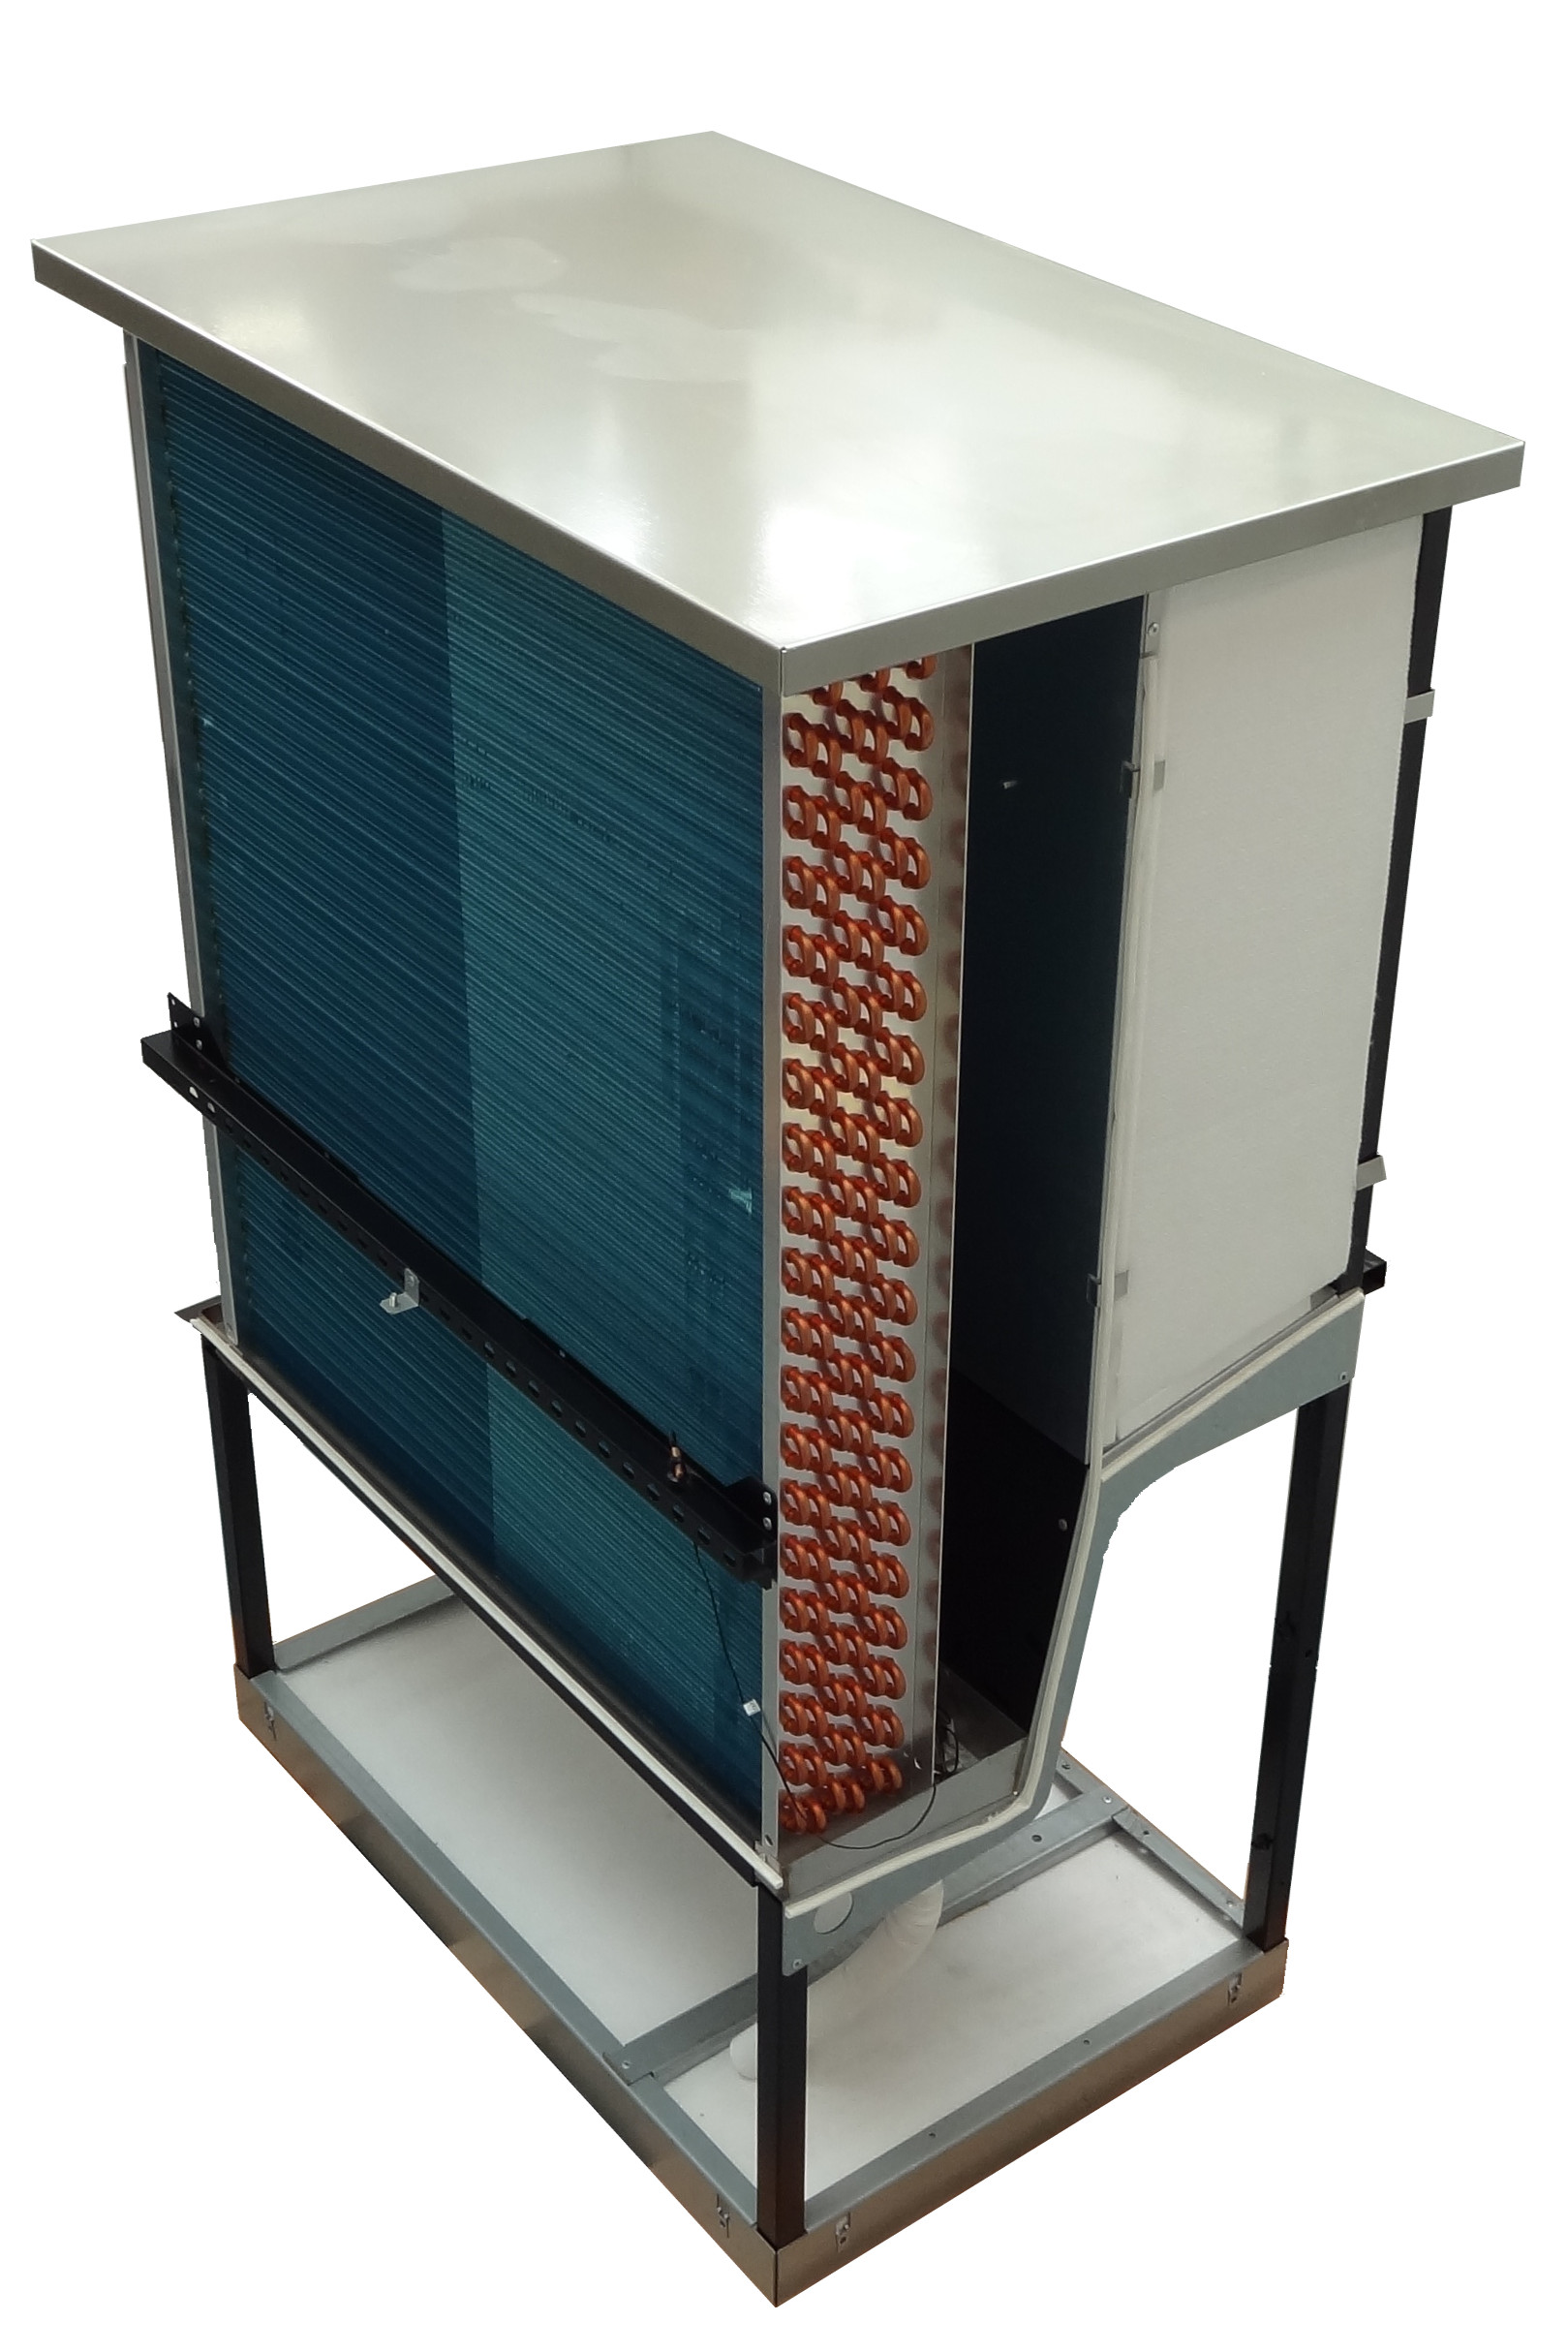
\includegraphics[height=8cm]{awp-chassis}}
  \subfloat[AWP 3D layout (bottom part)]{
    \label{fig:awp-3d-layout}
    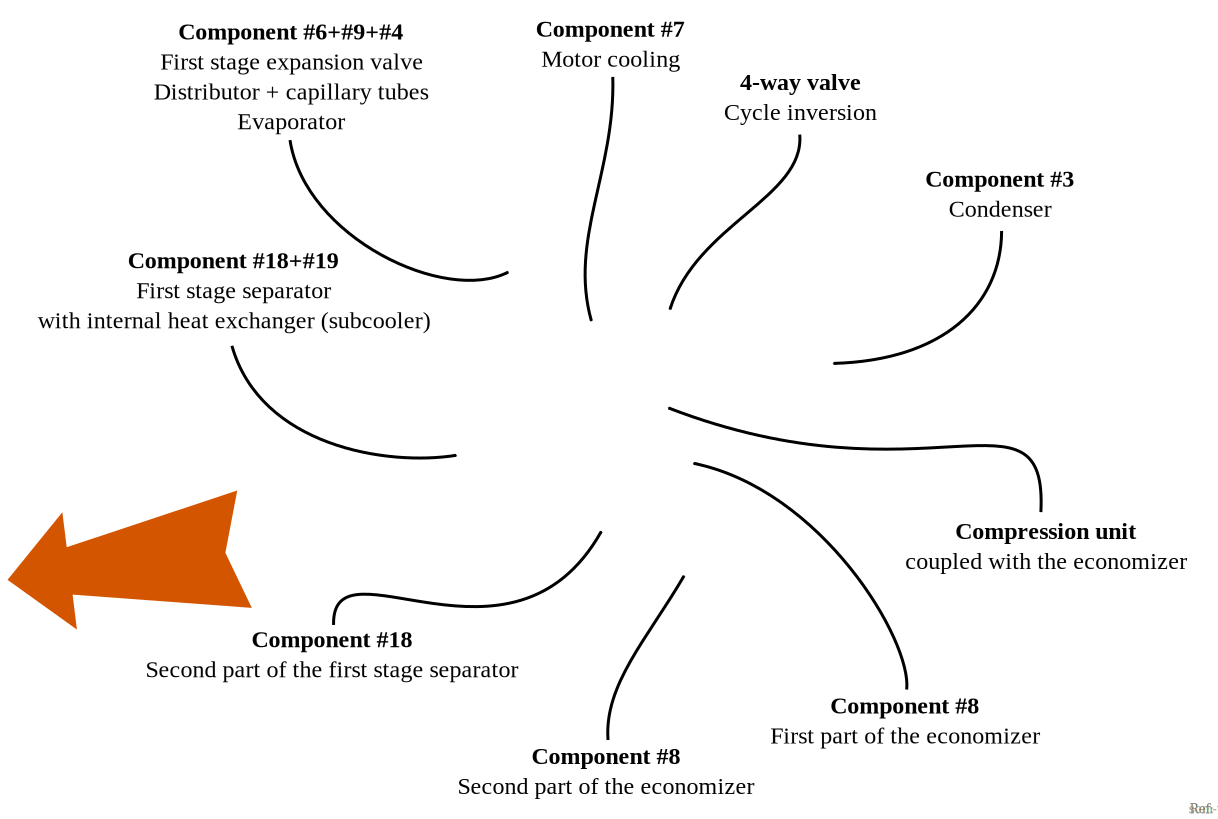
\includegraphics[height=7cm]{awp-3d-layout-commented}}
  \caption[Housing and 3D layout of the AWP circuits]{Housing and 3D
    layout of the AWP circuits, as they were expected to be built. The
    differences between the expected layout and the layout that has
    been tested are detailed in \cref{sec:awp-main-components}.}
  \label{fig:awp-housing-and-3d}
\end{figure}

\section{AWP components}
\label{sec:awp-main-components}

This section gives details of the main components in order to
make the understanding of the
\crefrange{sec:awp-model}{sec:awp-control-issues} easier. Further
details about the components and the topology of the circuits are give
in \cpref{chap:awp-components}.

\begin{figure}[htbp]
  \centering
  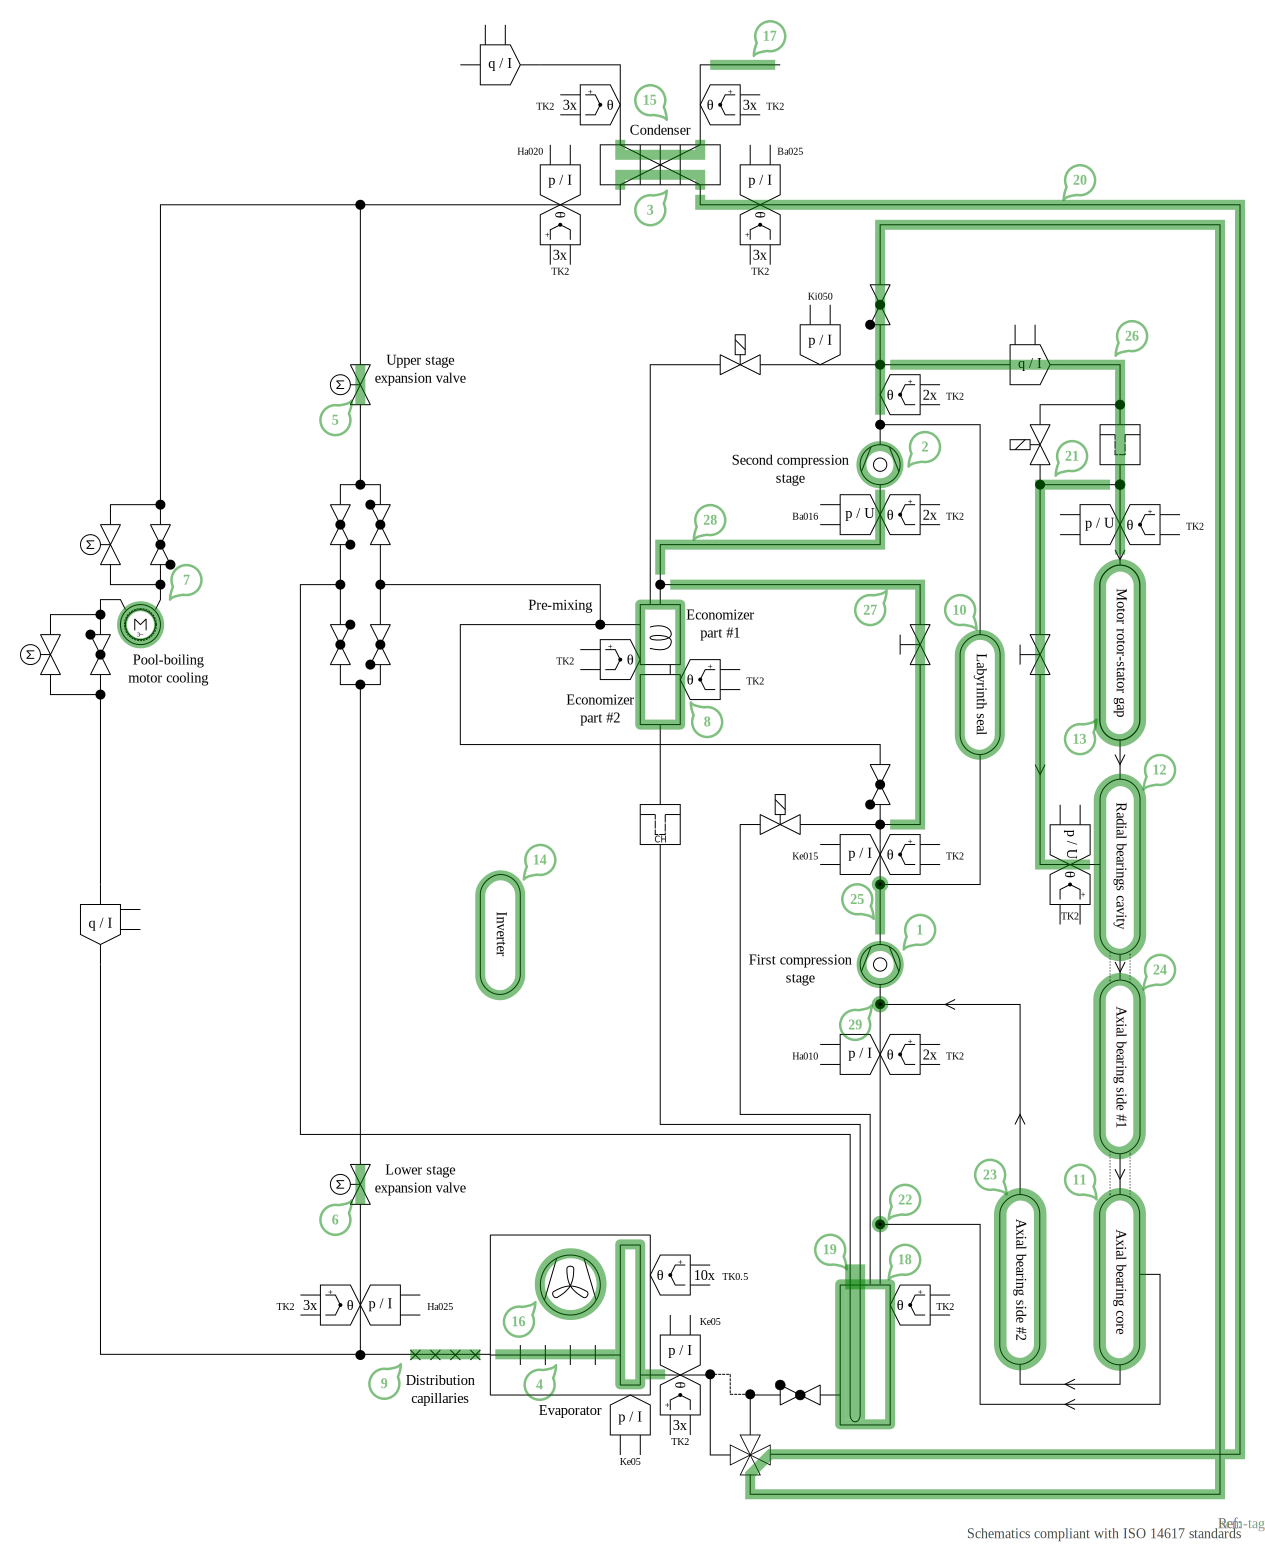
\includegraphics[width=1\textwidth]{awp-layout}
  \caption[AWP layout with components numbers]
  {AWP layout, with components numbers}
  \label{fig:awp-layout-model-numbers}
\end{figure}

\begin{figure}[htbp]
  \centering
  \includegraphics[width=0.65\textwidth]{awp-exp-analysis-model}
  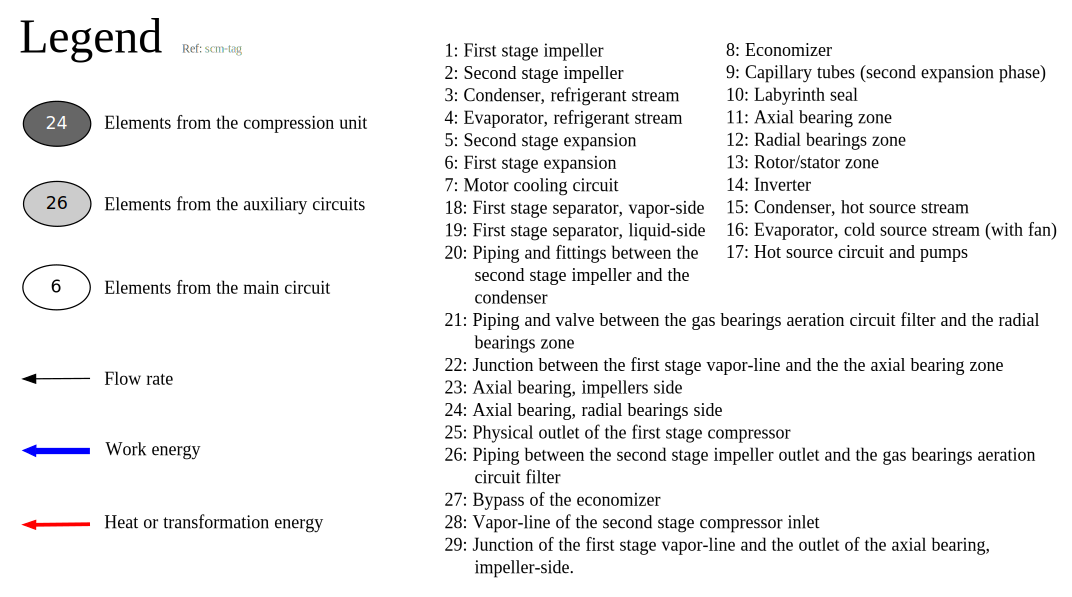
\includegraphics[width=0.95\textwidth]{awp-exp-analysis-model-legend}
  \caption[AWP model]{AWP model}
  \label{fig:awp-exp-analysis-model}
\end{figure}


This section only displays the details of some of the \AWP{} main
components. The level of detail given in this section corresponds to
the mandatory level needed to understand the contents of
\crefrange{sec:awp-model}{sec:awp-perfs}. \Cref{chap:awp-components}
extends those details and displays information about the components
that have not been described here, or only partially.

\subsection{Compression unit}
\label{sec:awp-cp-unit}

The compressor is a main component of vapor compression heat pump
cycles and has two main functions:

\begin{itemize}
\item Compress the refrigerant vapor from the evaporator so that the
  desired temperature and pressure can be maintained in the evaporator
  \citep[p.\,109]{dincer-kanoglu-2010a}.
\item Increase the pressure of the refrigerant vapor through the
  process of compression, simultaneously increasing the temperature of
  the refrigerant vapor \citep[p.\,109]{dincer-kanoglu-2010a} in order
  to meet the required condensation conditions
  \citep{rapin-desmons-2011a}.
\end{itemize}

Those two functions can not be fulfilled without the use of expansion
devices on liquid lines. The compressor role in the heat pump
prototype studied here is performed by a compression unit containing
the two compression stages, rotating at the same speed. The prototype
compression unit tested in the \AWP{} was the \textit{cp105}
compression unit, from the \textit{evo4} design family. Compression
units from \textit{evo1} and \textit{evo2} families have almost not
been tested in the \BWP{} or in the \AWP{}, as those units were not
ready for heat pump integration. Compression units from the
\textit{evo4} family were the first decently working prototypes that
have been available for tests\footnotep{More details about the
  compression unit history is given in \cref{sec:bwp-cp-unit}.}. They
started to be available during Spring 2012. One unit from the
\textit{evo4} family, the \textit{cp105} unit, has been tested in the
\AWP{} in May 2012. The datasets presented in this work have been
generated during that period. An other unit of this family,
\textit{cp101}, assembled before the \textit{cp105} unit, has been
tested later in the \BWP{}, in October 2013. Because of
confidentiality issues, the details of the design of the units or the
differences between the different compression unit design families can
not be exposed in this work and are only partially known by the author
himself. However, the structure of the \textit{cp105} unit and its
connections with the heat pump main and auxiliary circuits are
described in \cref{fig:cp105-struct-awp}. The main differences with
the version tested in the \BWP{} are:

\begin{description}
\item[Motor cooling configuration:] The motor cooling configuration
  tested on the \textit{cp105} unit was a pool-boiling
  configuration. In the \BWP{}, the motor was cooled down with a
  flow-boiling configuration\footnotep{Details about the motor cooling
    parts are given in \cref{sec:awp-motor-cooling-details}
    page~\pageref{sec:awp-motor-cooling-details}.}.
\item[Gas bearings aeration inlets/outlet configuration:] The gas
  bearings aeration circuit injects cold gas at the back of the
  compression unit (inlet \#1), after the motor (component
  \#13\footnotep{For components description and numbering, see
    \cref{fig:awp-layout-model-numbers,fig:awp-exp-analysis-model},
    page~\pageref{fig:awp-layout-model-numbers}
    and~\pageref{fig:awp-exp-analysis-model}.}), and in the radial gas
  bearings cavity (component \#12)
  (inlet \#2). The gas flows through the gap between the stator and
  the rotor, cooling down the two parts, and evacuating windage
  losses. This gas flow is mixed with the flow coming from the second
  inlet and leaves through the axial bearing of the motor
  side (component \#24) towards the
  outlet of the gas circuits, which is the middle of the set of axial
  bearings (component \#11). A share of
  this flow leaves by entering the axial bearing of the impeller
  side (component \#23)\footnotep{This
    gas path was not the one expected and this issue is discussed with
    further details in \cpref{sec:axial-is-reversed}.}.
\end{description}


\begin{figure}[htbp]
  \centering
  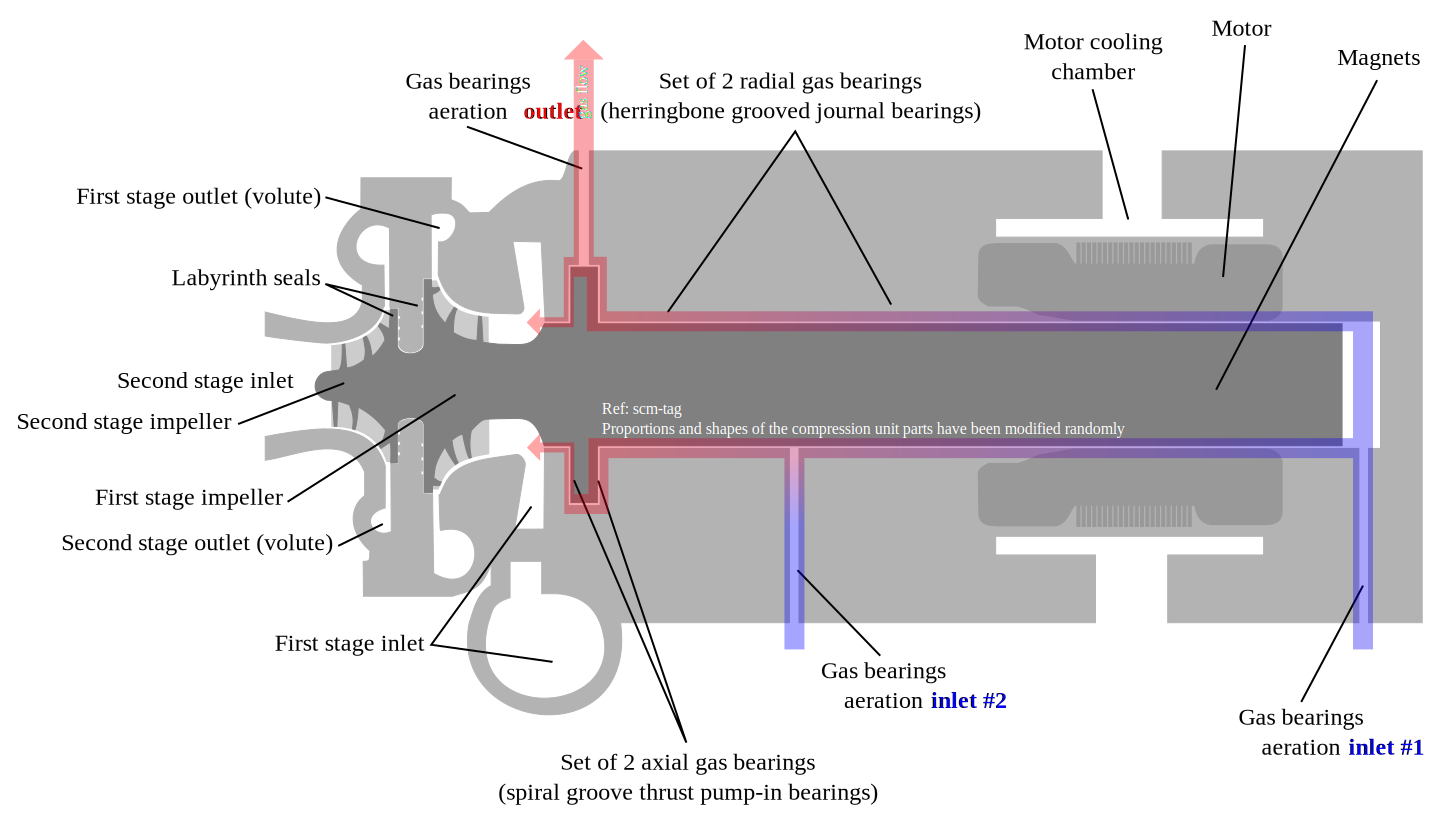
\includegraphics[width=\linewidth]{cp105-wheel-details-awp}
  \caption[Structure of the compressor unit with the AWP gas bearings
  aeration circuit I/O layout]{Structure of the twin-stage compressor
    unit with the AWP gas bearings aeration circuit inlets/outlets
    layout. Those inlets/outlets are different on the BWP, as
    illustrated in \cref{fig:cp101-struct-bwp}, page
    \pageref{fig:cp101-struct-bwp}.  Differences are stressed with a
    bold font.}
  \label{fig:cp105-struct-awp}
\end{figure}

\begin{figure}[htbp]
  \centering
  \subfloat[View of AWP]
  {\label{fig:awp-in-climate-chamber}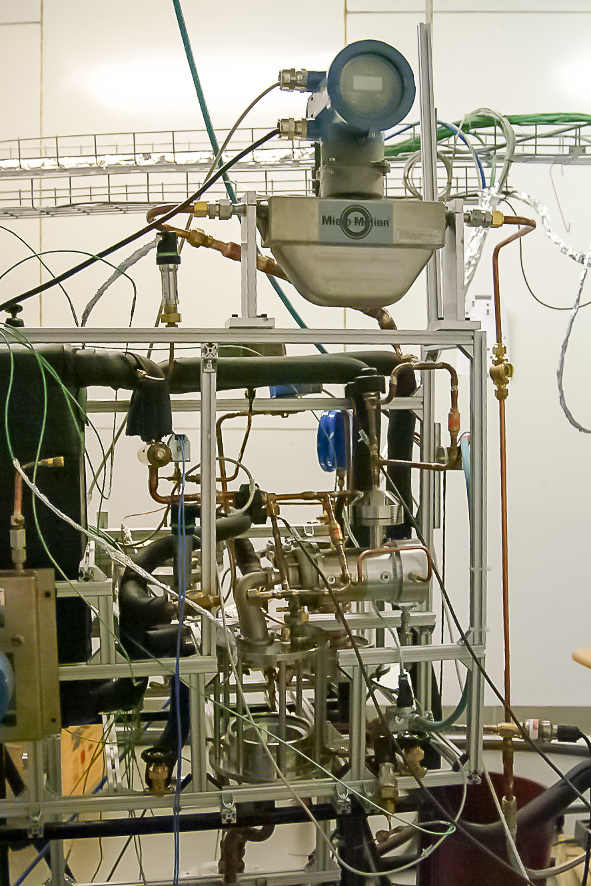
\includegraphics[height=10cm]{DSCF0217}}
  \hspace{1em}
  \subfloat[View of the evaporator]
  {\label{fig:awp-ev}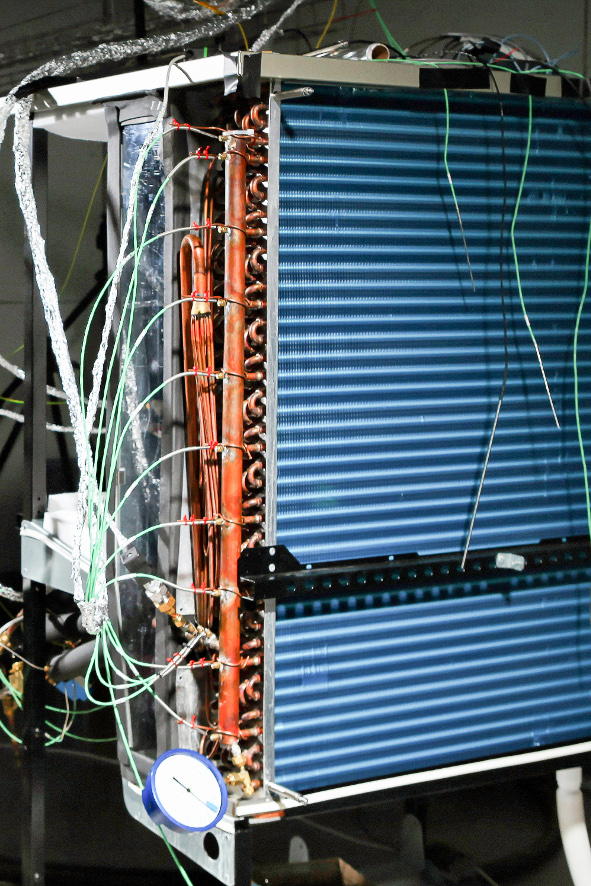
\includegraphics[height=10cm]{awp-ev}}
  \caption[Views of the AWP]{Views of the AWP. The extension of the
    economizer (component \#8) is located below its main part. The
    pipe connecting the two parts is visible at the bottom of the
    picture. Extra flow meters (one can be seen in
    \cref{fig:awp-in-climate-chamber}) have been added outside the
    original device housing, in order to understand the behavior of
    the prototype and characterize the system. The evaporator
    (\cref{fig:awp-ev}) is instrumented with a thermocouple per
    channel.}
  \label{fig:awp-views-in-climate-chamber}
\end{figure}

\begin{figure}[htbp]
  \centering
  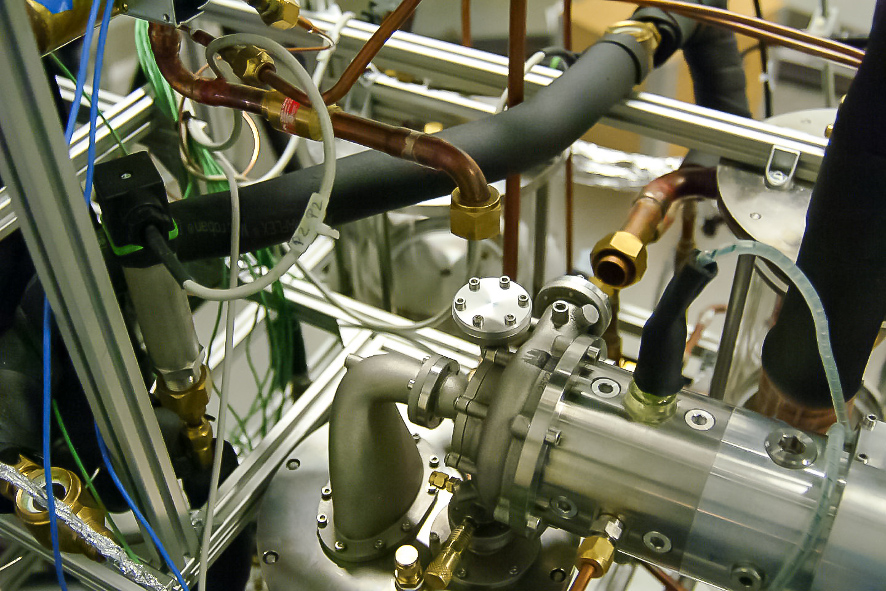
\includegraphics[width=12cm]{DSCF0215}
  \caption{Compression unit \textit{cp105}, being mounted in the AWP}
  \label{fig:cp105-being-mounted-in-awp}
\end{figure}


\subsection{Compression stage bypass systems}
\label{sec:awp-bypass}

Bypass circuits are mandatory auxiliary circuits in heat pumps
integrating the radial compression units. In the \AWP{}, each
compression stage is equipped with a bypass circuit consisting of a
manual needle valve, used to set the characteristics of the bypass,
and a solenoid valve for rapid bypass activation. This
solution had been chosen for cost-related reasons, and because the
crucial role of the bypass circuits dynamic response had not been
identified at the time. Fast electric needle valves are quite big and
expensive and were not appropriate if referred to the prototype
specification defined in \cref{sec:awp-specs}. The \BWP{} has been
equipped with such a valve for its bypass system, which is quite
different from the one used in the \AWP{}, as illustrated in
\cpref{fig:bypass-schematics}. The \BWP{} bypass system bypasses both
compression stages together, as described in
\cpref{sec:bwp-bypass-system} while the \AWP{} bypass system bypasses
each compression stage independently. However, being able to open or
close the bypass circuits independently in the \AWP{} does not make
them independent, as illustrated in
\cref{fig:awp-bypass-simple-layout}.


\subsection{Economizer}
\label{sec:awp-eco}

The \AWP{} is equipped with glass-made separator and economizer to
allow an easier monitoring and understanding of the refrigerant
distribution. This configuration allows for instance to see the
topology of the flow or to see if droplets appear at critical
locations. To prevent liquid management issues during the tests at the
laboratory, the inlet separator and the economizer should be able to
contain a good share of the refrigerant charge. When the heat pump
cycle is reversed for cooling or defrosting mode, part of the
refrigerant charge is likely to flow from the condenser to the
evaporator in a short time, due to the pressure difference between
those two components. This volume of liquid is likely to arrive in the
first stage inlet separator, consequently. In normal operation, the
liquid content of each heat exchanger is determined by its flow
conditions and characteristics (pinch diagram and flow pattern maps,
notably). The charge which is not contained in the heat exchangers at
a given time is collected in the economizer, which has to be able to
contain this charge while ensuring its liquid/gas separation function
properly. In order to decrease the impact of control mistakes during
the experiments, the volumes of the first stage compressor inlet
separator and of the economizer have been increased by a factor two by
duplicating them and by mounting the duplicates and the main parts
together\footnotep{See \cref{sec:awp-eco-appendix}
  page~\pageref{sec:awp-eco-appendix} for details.} in the prototype
(as illustrated in \cref{fig:awp-3d-layout}).

Gas/liquid separation issues were encountered in the economizer during
the experiments, so the design of the gas/liquid separation parts in
the economizer have evolved significantly during the experimental
investigation. The successive versions are detailed in
\cref{fig:awp-eco-gas-liq-sep-1-to-5}. The data presented in this
thesis work has been generated with the \AWP{} equipped with version
\#4 (before May 25\th{}, 2012) and version \#5 (after May 25\th{},
2012) of the economizer. An other action taken to solve the separation
issue was to move the second part of the economizer below the main
part, in order to increase the distance between the liquid level and
the second stage compressor inlet. The two components were connected
with a 20cm-long 3/4-inch pipe.

\begin{figure}[htbp]
  \centering \subfloat[Gas/liquid separation, version \#1 to \#4]
  {\label{fig:awp-eco-gas-liq-sep-1-to-4}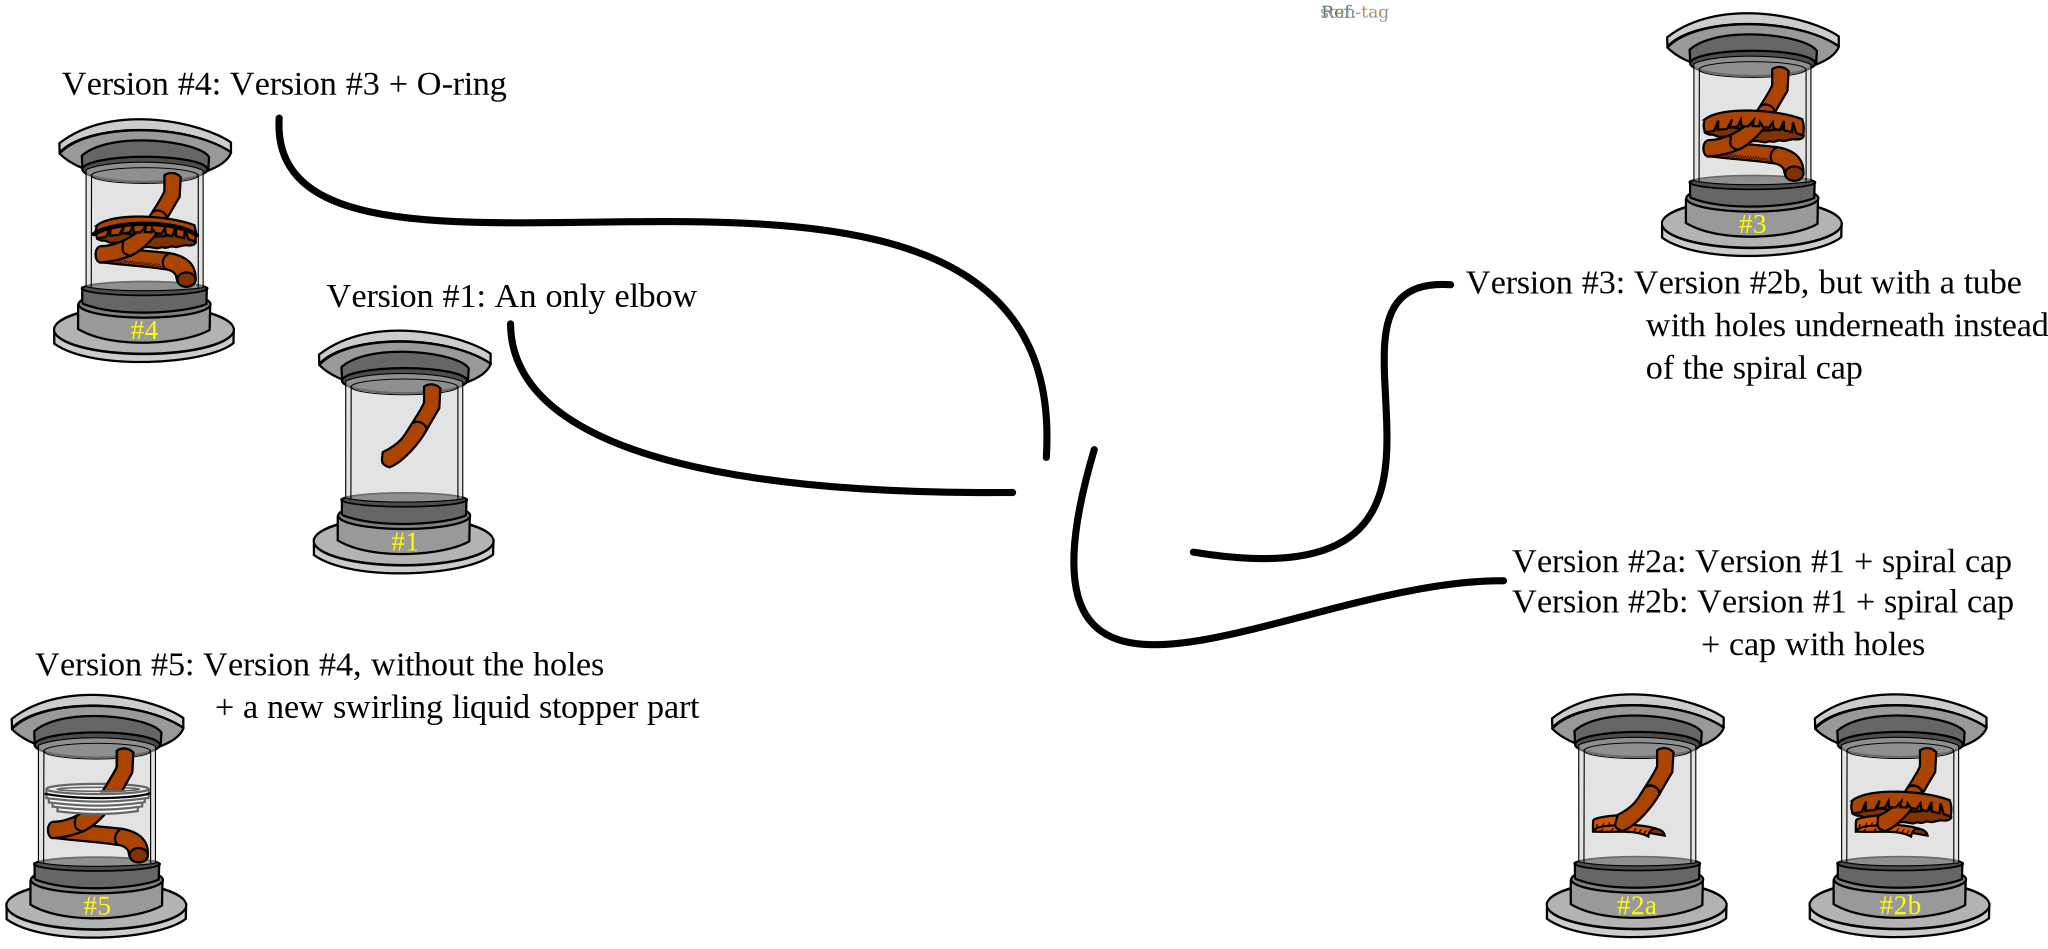
\includegraphics[width=\linewidth]{awp-eco-gas-liquid-sep-v1-to-v4}}
  \\\vspace{4em}
  \subfloat[Version \#5 (big central hole, with a seal and shapes to
  send the liquid back down the economizer on the sides)]
  {\label{fig:awp-eco-gas-liq-sep-5}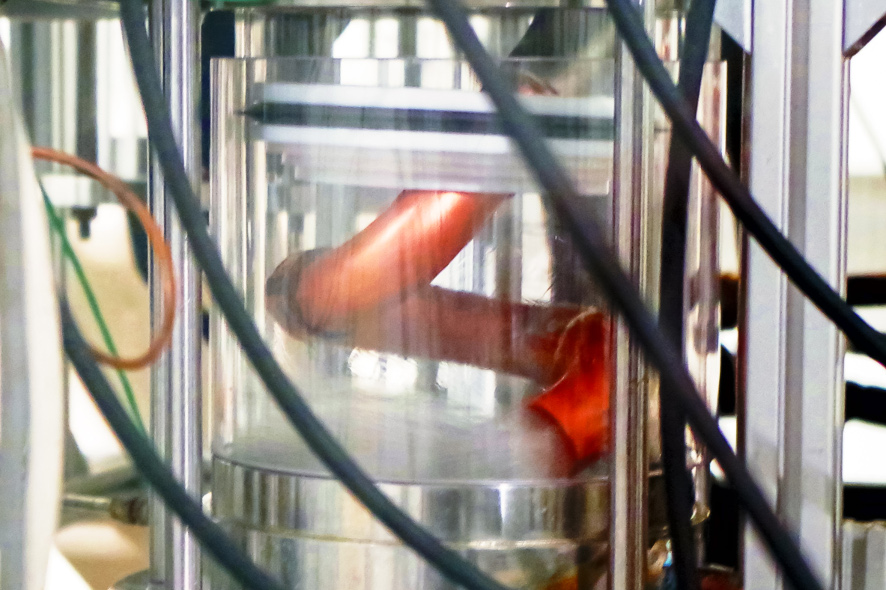
\includegraphics[width=12cm]{DSCF0172-mod}}
  \caption{AWP economizer version \#1 to \#5.}
  \label{fig:awp-eco-gas-liq-sep-1-to-5}
\end{figure}

\begin{figure}[htbp]
  \centering
  \begin{minipage}[r]{.49\linewidth}
    \begin{flushright}
      \subfloat[View \#1 ]{\label{fig:awp_assembly_1}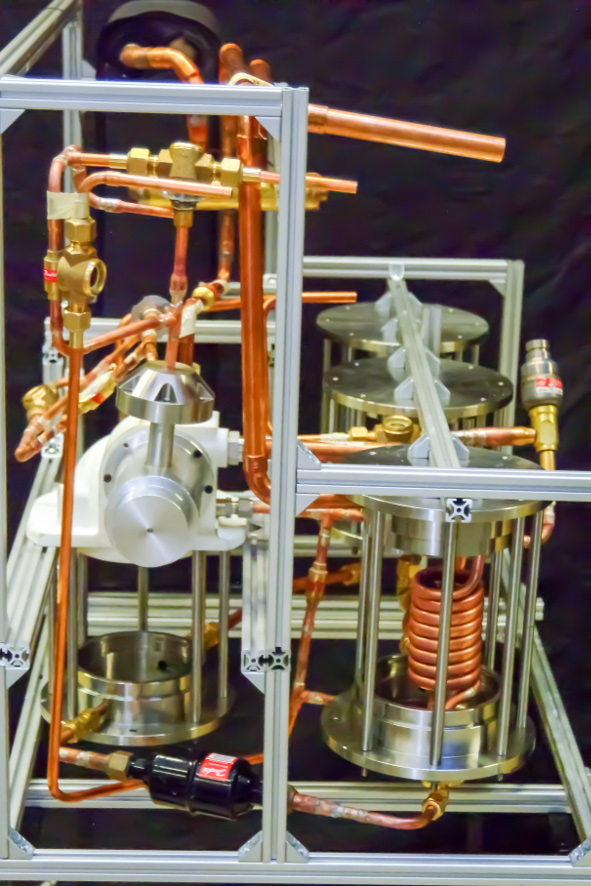
\includegraphics[height=11cm]{DSCF0016-mod}}
    \end{flushright}
  \end{minipage} \hfill
  \begin{minipage}[l]{.49\linewidth}
    \begin{flushleft}
      \subfloat[View \#2]{\label{fig:awp_assembly_2}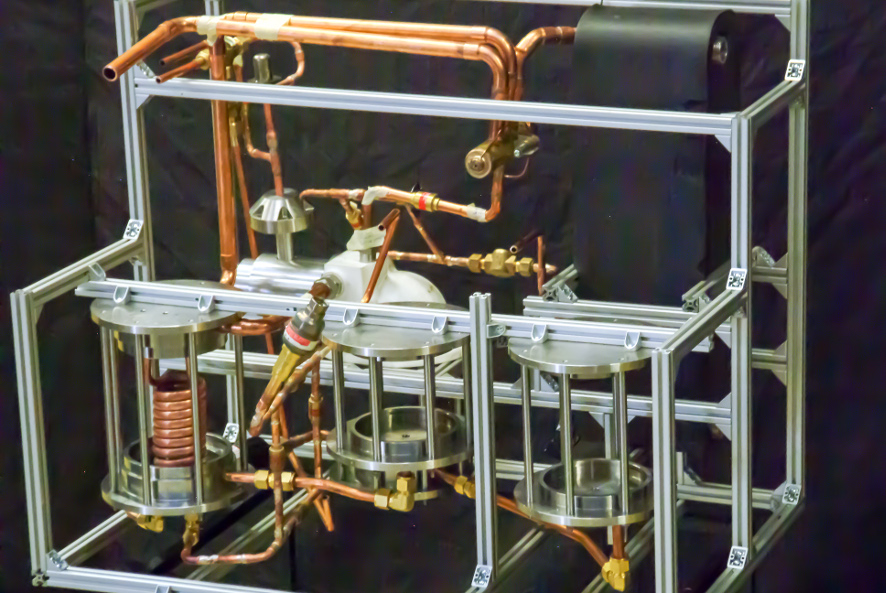
\includegraphics[height=5.07cm]{DSCF0017-mod}} \\
      \subfloat[View \#3]{\label{fig:awp_assembly_3}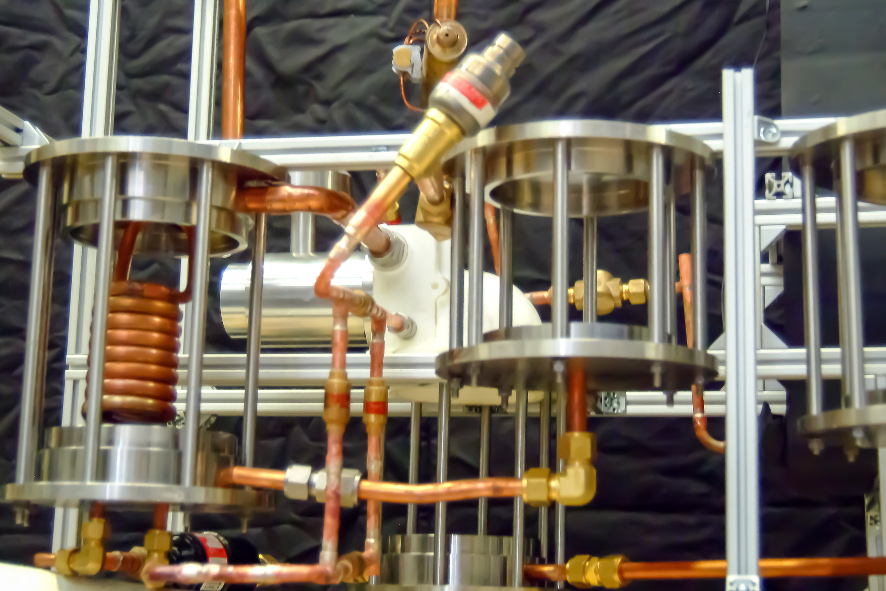
\includegraphics[height=5.07cm]{DSCF0002-mod}}
    \end{flushleft}
  \end{minipage}
  \caption{AWP assembly}
  \label{fig:awp_assembly}
\end{figure}

\begin{figure}[htbp]
  \centering \subfloat[Very low flow rate]
  {\label{fig:awp_eco_vlow_mf}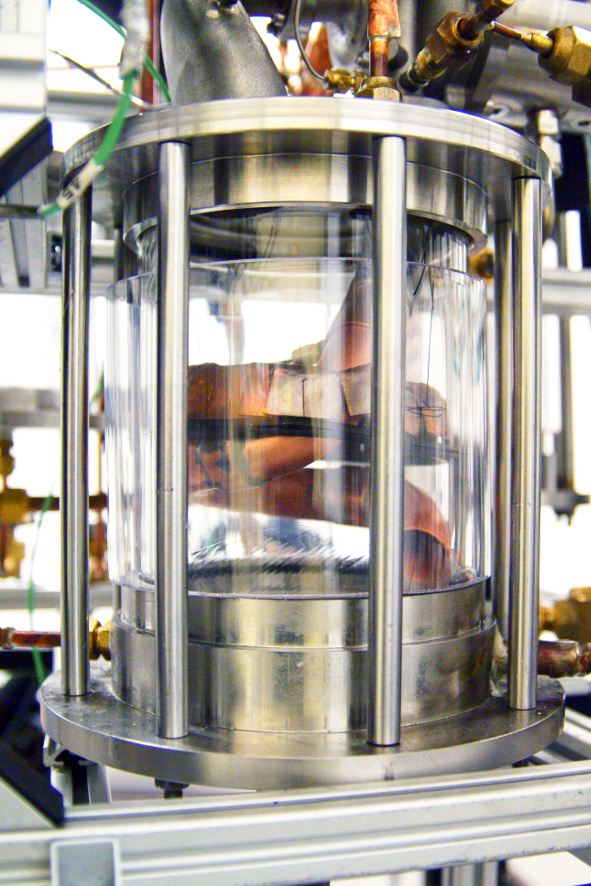
\includegraphics[width=0.45\linewidth]{DSCF0093-mod}}
  \hspace{1em} \subfloat[Liquid flowing up]
  {\label{fig:awp_eco_flow_up}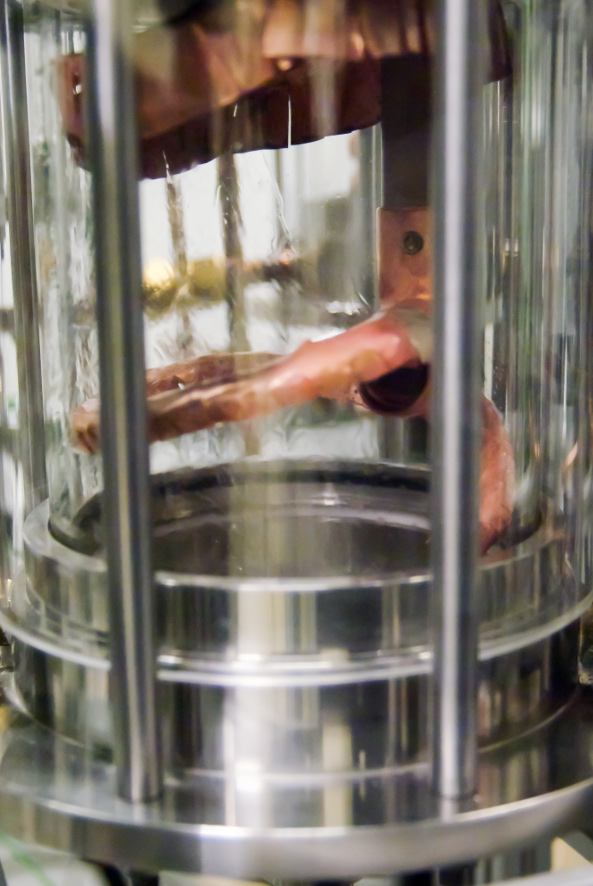
\includegraphics[width=0.45\linewidth]{DSCF0098_120krpm}}
  \\
  \subfloat[Low flow rate]
  {\label{fig:awp_eco_low_mf}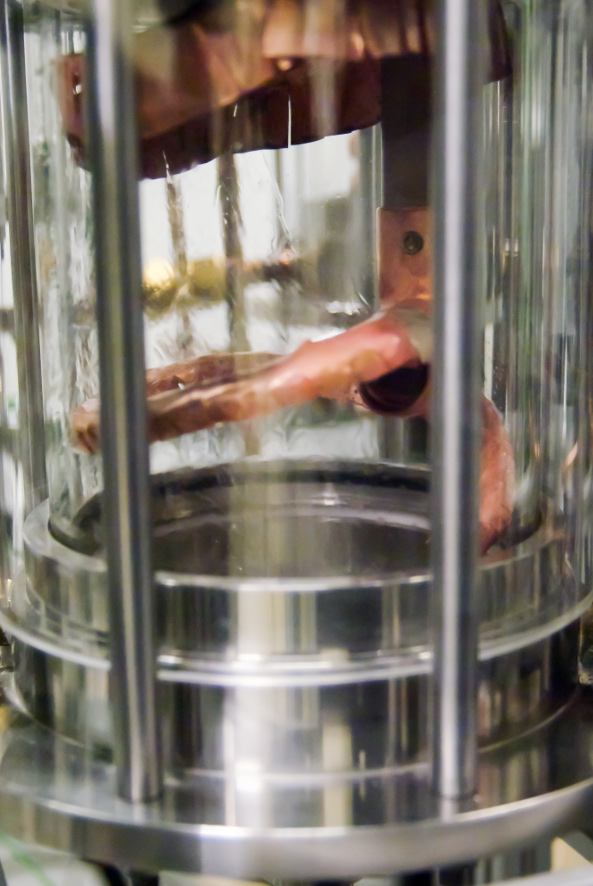
\includegraphics[height=70mm]{DSCF0098_120krpm}}
  \hspace{1em} \subfloat[Moderate flow rate]
  {\label{fig:awp_eco_mid_mf}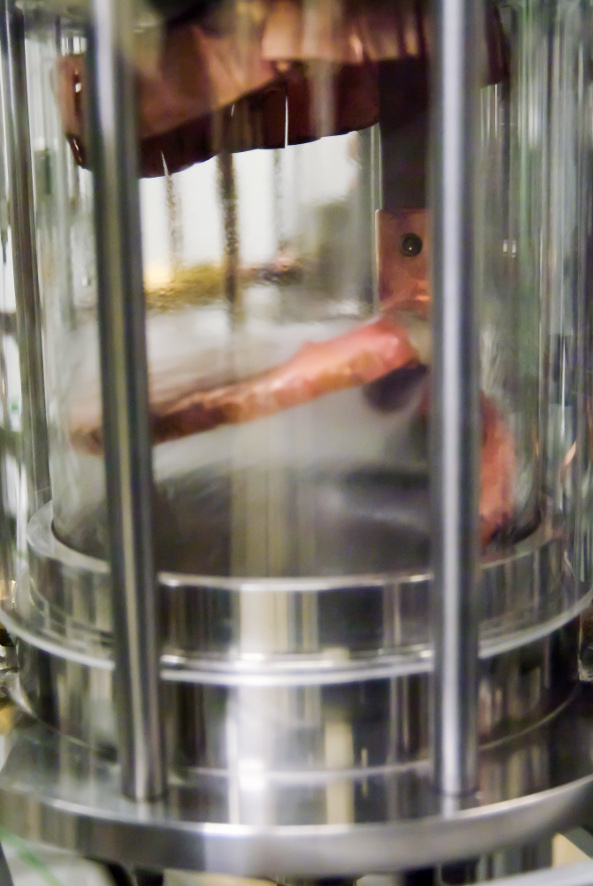
\includegraphics[height=70mm]{DSCF0095_120krpm}}
  \hspace{1em} \subfloat[High flow rate]
  {\label{fig:awp_eco_high_mf}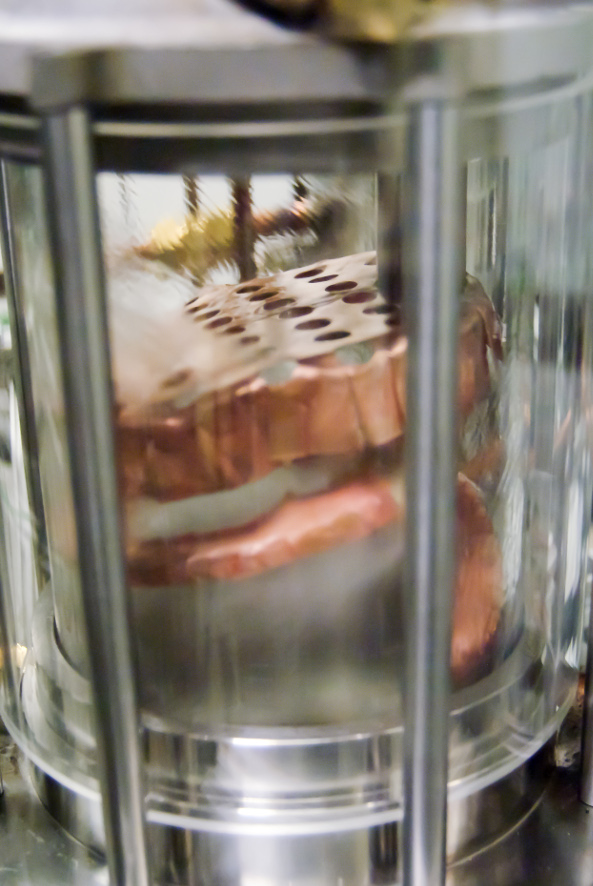
\includegraphics[height=70mm]{DSCF0070_110krpm}}
  \caption[Gas/liquid stream patterns with qualitative flow
  velocities]{Gas/liquid stream patterns with qualitative flow
    velocities. The gas/liquid separation assemblies used in this
    illustration are assemblies version \#2a, \#2b, and \#4.}
  \label{fig:awp-eco-flow-rates}
\end{figure}

\subsection{Evaporator}
\label{sec:awp-ev}

The evaporator of the \AWP{} is pictured on \cref{fig:awp-ev}. The air
ducting of the heat pump housing used as a base for the \AWP{} design
occurred to be designed with compactness in mind and has not been
designed for optimum air streams or noise reduction. The goal of the
designers was clearly to design a heat pump unit able to go through
the width of a conventional domestic doorway. As a result of those
design choices, the air stream distribution in the air ducting was far
from being satisfactory, as detailed in
\cref{sec:awp-issue-reducing-oh}. In order to try to compensate for
this issue, a plate drilled with holes in front of the evaporator
channels which had the lowest degree of superheat at their outlets has
been added at the inlet of the air ducting. This plate and its
influence on the superheating profile along the height of the
evaporator are detailed in \cref{sec:awp-issue-reducing-oh}.

\subsection{4-way valve}
\label{sec:awp-4way}

A 4-way reversing valve is included in the heat pump circuits in order
to switch between heating-mode, cooling-mode, and defrosting-mode. It
can be seen in \cref{fig:awp-4way-valve-in-circuits}. Such a valve
allows the condenser and evaporator to exchange their role in the heat
pump cycle, in order to defrost the evaporator during the heating
period, or for space cooling application. The flow of the refrigerant
in the exchangers is reversed and the roles of the exchangers are
exchanged. The valve is mounted on the suction line of the first
compression stage and the discharge line of the second compression
stage. The slide assembly inside the valve can translate to connect
the appropriate ports for the desired operation mode. It generates
additional pressure drops, a leakage flow and a heat exchange between
the discharge and the suction ports
\citep[p.\,4]{bertsch-hubacher-2002a}. This leakage has been measured
by \citet[p.\,39]{bertsch-hubacher-2002a} for a type of 4-way valve
very similar to the one used in the \AWP{} and have been measured
between 1 and 3 \si{\milli\gram\per\second\per\bar} with R134a. The
valve used in \AWP{} has been cleaned in order to remove any lubricant
contained within the valve\footnotep{The application here must be
  oil-free, as detailed in \cpref{sec:awp-issue-oil+corrosion}.},
which has certainly contributed to increase the leakage between the
suction and discharge ports, as the oil acts also as a sealant. This
leakage is neglected in the frame of this study. The 4-way valve in
the \AWP{} is the valve that was already present in the industrial
partner heat pump delivered to EPFL. As it had been sized for R407C,
this valve was slightly small to be used with R134a, as confirmed in
\cref{sec:awp-issue-4way}.

\begin{figure}[htbp]
  \centering
  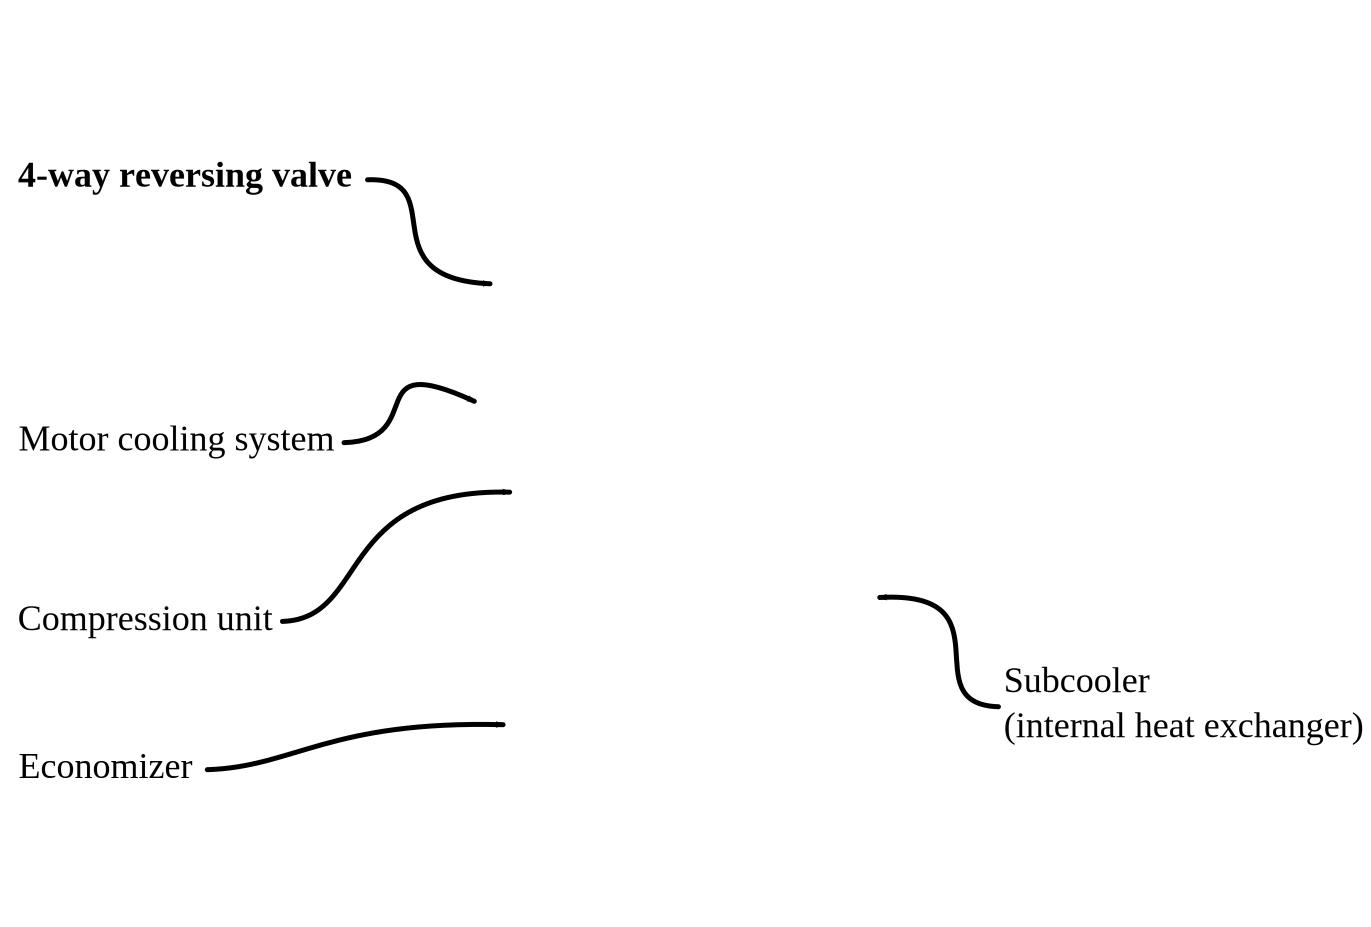
\includegraphics[width=15cm]{awp-4way-valve}
  \caption{View of the 4-way reversing valve in the heat pump circuits}
  \label{fig:awp-4way-valve-in-circuits}
\end{figure}


\section{Modeling}
\label{sec:awp-model}

The model proposed is based on the areas or physical elements of
interest in the \AWP{}. \Cref{fig:awp-layout-model-numbers} presents
the \AWP{} layout and \cref{fig:awp-exp-analysis-model} presents the
model itself. The set of equations deduced from analysis of the model
in \cref{fig:awp-exp-analysis-model} is detailed in
\cref{chap:awp-eqn}.

Following the procedure described in \cref{sec:methodo-models}, the
model is built with 29 components; 11 of them describe the compression
unit itself.

\section{Prototype performance}
\label{sec:awp-perfs}

A stable\footnotep{An OP is considered stable if it qualifies to
  defined conditions. See \cref{sec:stable-op}
  page~\pageref{sec:stable-op} for details.} \OP{} ensures that the
experimental setup is in a steady state, which allows to use the
modeling technique presented in \cpref{sec:methodo-models}. Indeed,
the data recorded were not enough to use a dynamic modeling approach,
but were appropriate for a steady state modeling approach. The maximum
rotor speed reached with the compressor unit is 180 krpm, which is the
maximum rotor speed of the compression unit, by design, and also the
maximum speed configured in the inverter. The maximum rotor speed
reached for a stable \OP{} is 171 krpm.

The first and the second \OP{}, A-6.8/W31.3 and A-7.0/W32.3, are two
similar \OP{}\footnotep{The first and second OP are detailed
  respectively in \cpref{sec:awp-exp-details-A-6.8/W31.3} and
  \cpref{sec:awp-exp-details-A-7.0/W32.3}.}, regarding temperature
levels. One has been measured with the 4-way reversing valve, one has
been measured without. The consequence of this modification of the
heat pump circuits is detailed in \cref{sec:awp-issue-4way}. The third
\OP{}\footnotep{The third OP is detailed in
  \cpref{sec:awp-exp-details-A-7.0/W35.6}.}, A-7.0/W35.6, yields the
highest temperature lift between the sources. It allows a comparison
of the \AWP{} with industrial products currently on the market, since
the \OP{} A-7/W35 is common \OP{} heat pump ranking and
comparison \citep{EN-14511-3}. The next three \OP{}\footnotep{Those 3
  OP are detailed respectively in
  \cpref{sec:awp-exp-details-A-0.5/W20.7},
  \cpref{sec:awp-exp-details-A-3.1/W29.5}, and
  \cpref{sec:awp-exp-details-A-6.6/W22.1}.}, A-0.5/W20.7, A-3.1/W29.5,
and A-6.6/W22.1, illustrate the gas temperature profile behavior
inside the compression unit, with the increase of the rotation
speed. This issue is documented in \cref{sec:awp-laby-hot-gas}.

\Cref{tab:awp-performances-summary} summarizes the main performance
indicators for the 6 stable \OP{}. The inverter is considered to be
inside the internal frontier in the model presented
\cref{fig:awp-exp-analysis-model}, since its efficiency is not
properly known. Indeed, it could be measured only once, with the
compressor unit running at 120 krpm, as the laboratory was not
equipped to perform high frequency three-phase power measurements on a
regular basis. Consequently, this measured efficiency of 85\% is
considered constant in this thesis work. The \COP{} is consequently
defined as expressed in \cpref{eq:COPh}, and considers the inverter to
be part of the internal system. \COP{}, as defined in \cref{eq:COPh},
does not take into account the pumps or the fan energy consumption
for the auxiliary fluids. The experimental results show differences of
temperature between the sources from 28.7 to 42.6 degrees and \COP{}
ranges from 2.19 to 4.02 in the stable \OP{} reached. The overall
exergy efficiencies, defined in \cpref{eq:eta_heatpump}, range from
26.3\% to 32.6\%. Those exergy efficiencies are considered low, as
they could have reached 30 to 40\% with better heat exchangers,
notably with a better evaporator\footnotep{The evaporator exergy
  efficiency $\eta_{ev}$, in the OP detailed in
  \cref{tab:awp-performances-summary}, ranges from 17\% to 34\% (see
  \cpref{sec:awp-issue-reducing-oh}) and is calculated with
  \cpref{eq:eta_ev_awp}. The subcooler exergy efficiency $\eta_{sc}$
  ranges from 0.4\% to 3\% (see \cpref{sec:awp-low-etaII-sc}) and is
  calculated with \cpref{eq:eta_sc}.}, improved
insulation\footnotep{The prototype was only partially insulated, as
  this can be seen on \cref{fig:awp-in-climate-chamber}
  page~\pageref{fig:awp-in-climate-chamber}.}, better control of the
auxiliary circuits\footnotep{The motor cooling flow was often not
  appropriate, as detailed in \cref{sec:awp-issue-motor-cooling}
  page~\pageref{sec:awp-issue-motor-cooling}, and the gas bearings
  aeration flow was not easy to set at a chosen value, as described in
  \cref{sec:awp-low-etaII-sc} page~\pageref{sec:awp-low-etaII-sc}.},
and better control of the subcooling and superheating
values\footnotep{Those values were not easily controlled, as explained
  in \cref{sec:awp-issue-control,sec:awp-issue-reducing-oh},
  page~\pageref{sec:awp-issue-control}.}. The most interesting \OP{}
is the \OP{} A-7.0/W35.6\footnotep{More details about this specific OP
  are given in \cref{sec:awp-exp-details-A-7.0/W35.6}
  page~\pageref{sec:awp-exp-details-A-7.0/W35.6}.}, which allows to
compare the \AWP{} performance with industrial products performance
using conventional technology, even if the comparison is not very
accurate, as the prototype tests were not strictly performed in the
conditions imposed by the standards relative to performance
measurement of heat pumps with electrically driven compressors for
space heating \& cooling
applications \citep{EN-14511-1,EN-14511-2,EN-14511-3,EN-14511-4,EN-14825}
\footnotep{Acoustic measurements conditions are detailed in other
  standards \citep{EN-12102,EN-ISO-9614-1}.}. Notably, the fan and pump
electrical powers were not taken in account \citep[sec.\,4.1.4 and
4.1.6]{EN-14511-3}, the condenser water temperature difference was of
\num{6.84}\si{\kelvin}, instead of
5\si{\kelvin} \citep[tab.\,12]{EN-14511-2}\footnotep{The standard
  condenser inlet/outlet water for this OP are 30\si{\degreeCelsius}
  at the inlet and 35\si{\degreeCelsius} at the outlet.}, and the
condenser inlet temperature was not exactly at
\num{35.0}\si{\degreeCelsius}, but at
\num{35.6}\si{\degreeCelsius}. Nonetheless, it appears that the \AWP{}
performs close to the devices currently on the market, as it can be
seen in \cref{tab:awp-indus-products-comparison}. Indeed, the \AWP{}
performance is a little lower than the devices it compares with
(\COP{} is 0.2 to 0.5 points lower). Reaching this level of
performance is encouraging, since even this first working prototype,
far from being a complete optimized industrial version, already ranks
close to the models currently on the market. In addition to the
drawbacks mentioned above, the prototype topology was burst around in
order to include measurement capabilities, creating pressure drop. As
illustrated in \cref{fig:awp-A-7.0/W35.6-sankey-energy}, about 6\% of
the energy was dissipated in the environment during this experiment
A-7.0/W35.6. Those 6\% include the heat losses of the
inverter (component \#14). This heat
energy could be also recovered by the thermodynamic cycle, for
instance, as it is already the case for the motor heat
losses. Moreover, the control issues detailed in
\cref{sec:awp-control-issues} have also a negative influence on the
prototype performance. As a consequence, even if they are
comparatively low, the performance reached with this first working
prototype is considered very promising and constitutes a breakthrough
in the domain.

\begin{figure}[htbp]
  \centering
  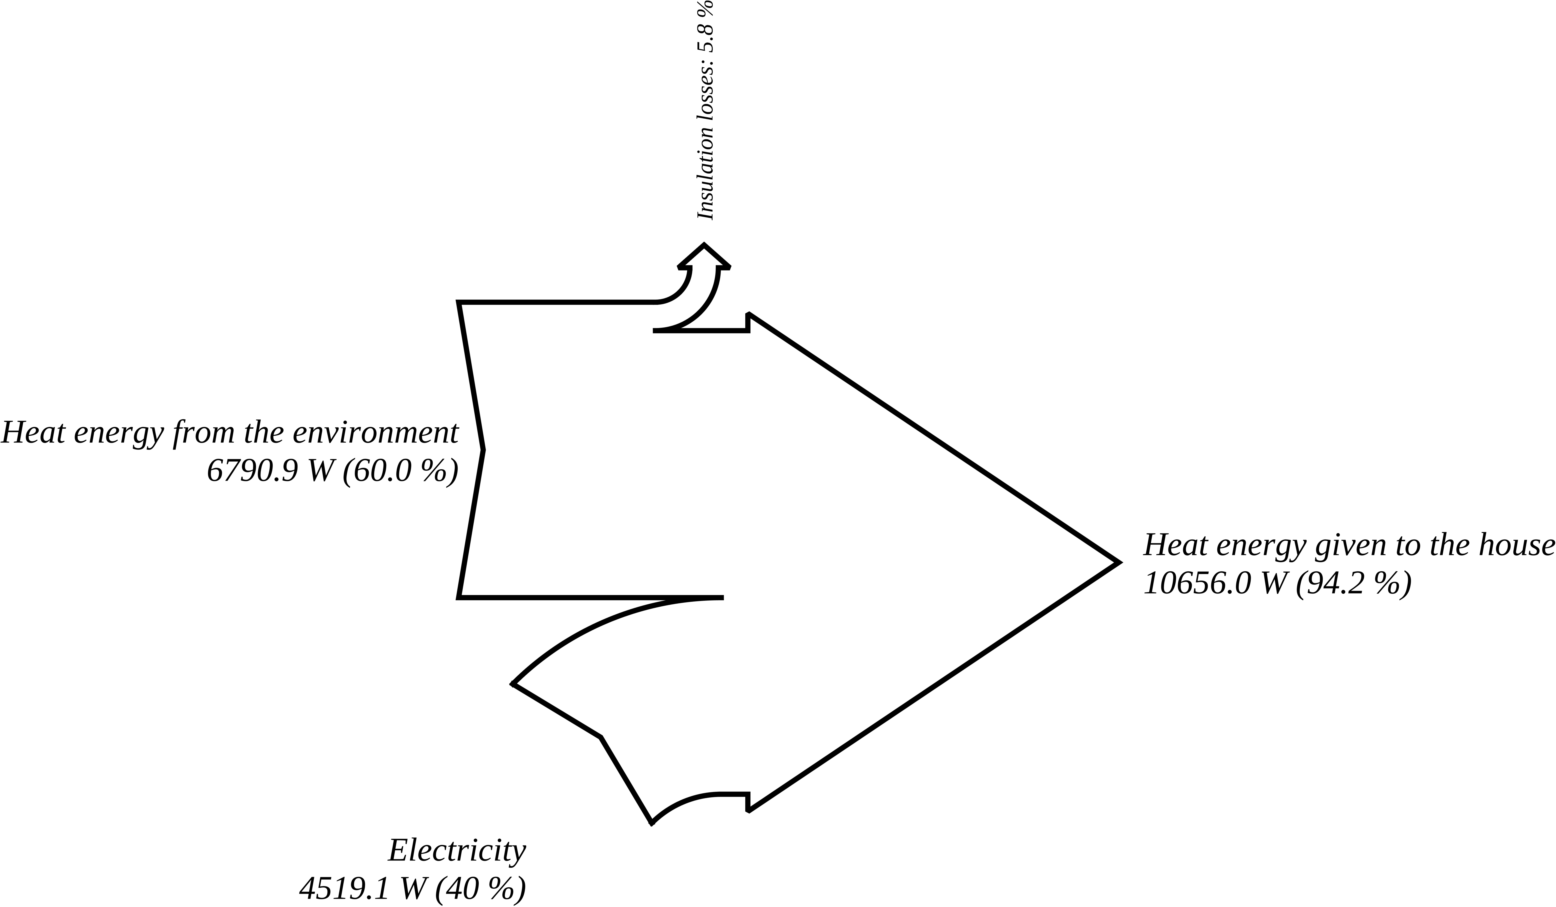
\includegraphics[width=1\textwidth]{awp-energy-sankey-awp-20120525-150822-151122}
  \caption{A-7.0/W35.6 - Sankey diagram for heat pump energy balance (internal frontier)}
  \label{fig:awp-A-7.0/W35.6-sankey-energy}
\end{figure}


\begin{table}[htbp]
  \begin{center}
    \footnotesize
    \begin{tabular}{lccccccc}
\toprule
\OP{} \# & & \#1 & \#2 & \#3 & \#4 & \#5 & \#6 \\
\OP{} & & A-6.8/W31.3 & A-7.0/W32.3 & A-7.0/W35.6 & A-0.5/W20.7 & A-3.1/W29.5 & A-6.6/W22.1 \\
Data & & \cref{sec:awp-exp-details-A-6.8/W31.3} & \cref{sec:awp-exp-details-A-7.0/W32.3} & \cref{sec:awp-exp-details-A-7.0/W35.6} & \cref{sec:awp-exp-details-A-0.5/W20.7} & \cref{sec:awp-exp-details-A-3.1/W29.5} & \cref{sec:awp-exp-details-A-6.6/W22.1} \\
Speed & & 170 krpm & 160 krpm & 171 krpm & 130 krpm & 153 krpm & 160 krpm \\
\midrule
 $ \epsilon_h $ & -  & $ \num{2.19} \pm \num{0.04} $ & $ \num{2.69} \pm \num{0.03} $ & $ \num{2.36} \pm \num{0.03} $ & $ \num{4.02} \pm \num{0.06} $ & $ \num{3.10} \pm \num{0.04} $ & $ \num{2.67} \pm \num{0.05} $ \\
 $ \eta_{heatpump} $ & \%  & $ \num{26.3} \pm \num{0.7} $ & $ \num{32.6} \pm \num{0.5} $ & $ \num{30.5} \pm \num{0.5} $ & $ \num{26.6} \pm \num{0.8} $ & $ \num{31.0} \pm \num{0.6} $ & $ \num{25.2} \pm \num{0.7} $ \\
 $ \eta_{motor} $ & \%  & $\underline{88.99}$ & $\underline{82.34}$ & $\underline{91.92}$ & $\underline{88.00}$ & $\underline{91.67}$ & $\underline{90.43}$ \\
 $ \eta_{cp1} $ & \%  & $ \num{59} \pm \num{40} $ & $ \num{63} \pm \num{36} $ & $ \num{62} \pm \num{37} $ & $ \num{76} \pm \num{23} $ & $ \num{74} \pm \num{26} $ & $ \num{71} \pm \num{30} $ \\
 $ \eta_{s,\,cp1} $ & \%  & $ \num{88} \pm \num{12} $ & $ \num{88} \pm \num{12} $ & $ \num{88} \pm \num{11} $ & $ \num{93} \pm \num{7} $ & $ \num{92} \pm \num{7} $ & $ \num{93} \pm \num{7} $ \\
 $ \eta_{cp2} $ & \%  & $ \num{83} \pm \num{17} $ & $ \num{80} \pm \num{19} $ & $ \num{59} \pm \num{16} $ & $ \num{66} \pm \num{34} $ & $ \num{75} \pm \num{24} $ & $ \num{60} \pm \num{30} $ \\
 $ \eta_{s,\,cp2} $ & \%  & $ \num{89} \pm \num{11} $ & $ \num{88} \pm \num{12} $ & $ \num{82} \pm \num{18} $ & $ \num{89} \pm \num{11} $ & $ \num{88} \pm \num{11} $ & $ \num{86} \pm \num{13} $ \\
 $ \eta_{cd} $ & \%  & $ \num{94} \pm \num{3} $ & $ \num{92} \pm \num{2} $ & $ \num{92} \pm \num{3} $ & $ \num{89} \pm \num{3} $ & $ \num{90} \pm \num{2} $ & $ \num{93} \pm \num{4} $ \\
 $ \eta_{ev} $ & \%  & $ \num{17} \pm \num{17} $ & $ \num{31} \pm \num{31} $ & $ \num{34} \pm \num{34} $ & $ \num{29} \pm \num{29} $ & $ \num{20} \pm \num{20} $ & $ \num{30} \pm \num{30} $ \\
 $ \eta_{sc} $ & \%  & $ \num{1} \pm \num{1} $ & $ \num{2} \pm \num{2} $ & $ \num{2} \pm \num{2} $ & $ \num{3} \pm \num{3} $ & $ \num{3} \pm \num{3} $ & $ \num{0.4} \pm \num{0.4} $ \\
 $ \dot{Y}_{3 \rightarrow 15} $ & \si{\watt} & $ \num{7367} \pm \num{138} $ & $ \num{1.0458e+04} \pm \num{134} $ & $ \num{1.0656e+04} \pm \num{137} $ & $ \num{9010} \pm \num{130} $ & $ \num{1.0252e+04} \pm \num{134} $ & $ \num{7363} \pm \num{125} $ \\
 $ \dot{Y}_{16 \rightarrow 4} $ & \si{\watt} & $ \num{4278} \pm \num{138} $ & $ \num{7144} \pm \num{136} $ & $ \num{6791} \pm \num{152} $ & $ \num{7102} \pm \num{131} $ & $ \num{7398} \pm \num{149} $ & $ \num{4875} \pm \num{174} $ \\
 $ \dot{E}_{el \rightarrow 14} $ & \si{\watt} & $ \pmb{\num{3367.4} \pm \num{0.5}} $ & $ \pmb{\num{3881.4} \pm \num{0.4}} $ & $ \pmb{\num{4519.1} \pm \num{0.4}} $ & $ \pmb{\num{2243.5} \pm \num{0.4}} $ & $ \pmb{\num{3310.7} \pm \num{0.4}} $ & $ \pmb{\num{2758.5} \pm \num{0.4}} $ \\
\bottomrule
\end{tabular}

  \end{center}
  \caption{Overall performance of the AWP and its main components}
  \label{tab:awp-performances-summary}
\end{table}

\begin{table}[htbp]
  \begin{center}
    \footnotesize
    \begin{tabular}{lccccc}
  \toprule
  Brand \& Model / - & $\dot{E}_{el}$ / \si{\kilo\watt} & $\dot{Y}_{cd}$ / \si{\kilo\watt} & $\epsilon_h$ / - & Noise level / dB(A) & current type / - \\
  \midrule
  LG Therma V & \multirow{2}{*}{\num{4.27}} & \multirow{2}{*}{\num{10.69}} & \multirow{2}{*}{\num{2.5}} & \multirow{2}{*}{\num{70}} & \multirow{2}{*}{400V – 50Hz} \\
  \textit{Model HU143U31} &&&&&\\
  Ciat Aqualis2+ 65 HT & \multirow{2}{*}{\num{3.89}} & \multirow{2}{*}{\num{10.7}} & \multirow{2}{*}{\num{2.75}} & \multirow{2}{*}{\num{73.5}} & \multirow{2}{*}{230V – 50Hz} \\
  \textit{Model 7321653} &&&&&\\
  Panasonic Aquarea Kompakt & \multirow{2}{*}{\num{4}} & \multirow{2}{*}{\num{10.7}} & \multirow{2}{*}{\num{2.68}} & \multirow{2}{*}{\num{69}} & \multirow{2}{*}{400V – 50Hz} \\
  \textit{Model WH-MDC14C9E8} &&&&&\\
  Atlantic Alféa Hybrid Duo Gas 11 Tri & \multirow{2}{*}{\num{4.28}} & \multirow{2}{*}{\num{10.8}} & \multirow{2}{*}{\num{2.52}} & \multirow{2}{*}{\num{66}} & \multirow{2}{*}{400V – 50Hz} \\
  \textit{Model WOYK112LTC} &&&&&\\
  Air/Water heat pump Prototype & \multirow{2}{*}{\num{4.5}} & \multirow{2}{*}{\num{10.7}} & \multirow{2}{*}{\num{2.36}} & \multirow{2}{*}{N/A} & \multirow{2}{*}{400V – 50Hz} \\
  \textit{AWP} &&&&&\\
  \midrule
  Brand \& Model / - &  Refrigerant / - & Type / - & \textit{cp} type / - & \textit{cp} stages / - & Reversibility / - \\
  \midrule
  LG Therma V & \multirow{2}{*}{R410A} & \multirow{2}{*}{Split} & \multirow{2}{*}{Rotary} & \multirow{2}{*}{Single} & \multirow{2}{*}{Not reversible} \\
  \textit{Model HU143U31} &&&&&\\
  Ciat Aqualis2+ 65 HT & \multirow{2}{*}{R410A} & \multirow{2}{*}{Monobloc} & \multirow{2}{*}{Scroll} & \multirow{2}{*}{Single} & \multirow{2}{*}{Reversible} \\
  \textit{Model 7321653} &&&&&\\
  Panasonic Aquarea Kompakt & \multirow{2}{*}{R410A} & \multirow{2}{*}{Monobloc} & \multirow{2}{*}{Rotary} & \multirow{2}{*}{Single} & \multirow{2}{*}{Reversible} \\
  \textit{Model WH-MDC14C9E8} &&&&&\\
  Atlantic Alféa Hybrid Duo Gas 11 Tri & \multirow{2}{*}{R410A} & \multirow{2}{*}{Split} & \multirow{2}{*}{Rotary} & \multirow{2}{*}{Single} & \multirow{2}{*}{Not reversible} \\
  \textit{Model WOYK112LTC} &&&&&\\
  Air/Water twin-stage heat pump Prototype & \multirow{2}{*}{R134a} & \multirow{2}{*}{Monobloc} & \multirow{2}{*}{Radial} & \multirow{2}{*}{Twin} & \multirow{2}{*}{Reversible}\\
  \textit{AWP} &&&&&\\
  \bottomrule
\end{tabular}

  \end{center}
  \caption[AWP and similar industrial domestic heat pumps coefficient
  of performance]{AWP and similar industrial domestic Air/Water heat
    pumps, currently on the market, \COP{} for the
    OP A-7/W35. Noise level corresponds to the external side sound
    level envelope. The Air/Water heat pumps \COP{} takes in account
    the defrosting process. The \AWP{} \COP{} does not include the
    defrosting process.}
  \label{tab:awp-indus-products-comparison}
\end{table}

\section{Design issues}
\label{sec:awp-design-issues}

This section details the encountered issues which are related to
\AWP{} layout design or topology deficiencies. Those deficiencies have
a negative influence on the prototype efficiency and performance.


\subsection{Gas forced to flow reversely in one side of
  the axial bearing}
\label{sec:axial-is-reversed}

The compressor thrust bearing is a two sided inward pumping spiral
groove thrust bearing. Under normal operating conditions such a
bearing is known for generating a gas flow from the bearings outside
diameter towards the bearings inside diameter. As described in
\cref{sec:awp-cp-unit}, this normal behavior is not observed in
component \#24, which is one side of the set of axial
bearings. Indeed, the gas bearings aeration circuit was set as
described in \cref{fig:cp105-struct-awp}. The appropriate setting is
described in \cpref{fig:cp101-struct-bwp}. A comparison of the normal
setting and the setting used in the \AWP{} shows that the outlet of
the gas bearings aeration circuit in the compression unit is connected
as an inlet. This means that the gas can only flow from the components
\#13 and \#12 inlets to component \#11 outlet through component \#24,
in the reverse way regarding bearing flow. The flow here is imposed by
the pressure levels in the circuit. The compressor has been plugged in
this way following the industrial partner requirements, and as the
internal design of the compression unit was unknown by the author. The
industrial partner was expecting to solve the issue documented in
\cref{sec:awp-P-balance} by plugging in the compressor this way.

\subsection{Excess of compressor thrust forces during
  deceleration}
\label{sec:awp-P-balance}

In steady state operation, the heat pump circuit has 3 pressure
levels. The high pressure zone is located between the outlet of
the second stage compressor and the inlet of the second stage
expansion valve. The intermediate pressure zone is located between the
two compression stages, including the economizer, and the low pressure
zone is located between the outlet of the first stage expansion valve
and the inlet of the first stage compressor. The larger is the
temperature difference between the condenser outlet and the evaporator
inlet, the larger is the difference of pressure level between the
zones.

When the compressor unit decelerates, the rotor speed decreases quite
fast, since the rotor is mechanically loaded by the compressor
work. In less than 2 seconds, the rotor speed drops below 100
krpm. Below 30 krpm, bearing touch-down occurs. Between 60 and 80
krpm, there is a dangerous operation zone, in particular if there is a
high pressure level difference between the zones. This is typically
the case in a running heat pump cycle, where the pressure levels are
determined by the temperature levels of the sources. Depending on the
design of the heat pump circuits, pressure level differences can also
be observed in the compression unit at specific times. As differences
of pressure levels in the compression unit induce thrust forces on the
axial bearing, and as both the bearing stiffness and load capacity
increase with rotor speed, there are situations where the external
force applied on the bearings might be high for their nominal load
capacity, especially with an unexpected reversed flow on one side of
the bearing.

When the \AWP{} runs at a given \OP{}, the pressure across the second
stage compressor varies from intermediate level to high pressure
level, through the second stage impeller. The pressure at the first
stage compressor varies from low level to intermediate pressure level,
through the first stage impeller. The pressure level in the radial
bearings cavity and at the back of the compressor unit is close to low
pressure level\footnotep{This is for minimizing the bearings and motor
  windage losses.}. When the compression unit decelerates abruptly (in
case of uncareful stop, which means stopping the prototype without
decreasing the gap between the temperature levels of the sources,
emergency stop, or power failure), the bypass circuits of the
compression stages\footnotep{See \cpref{sec:awp-bypass} for details
  about the bypass circuits.} are open in order to avoid the surge
phenomenon\footnotep{See \cpref{sec:op-domain} for details about the surge
  phenomenon.}. As the rotor speed decreases, it reaches the dangerous
zone described above, the pressure level in the second compression
stage rapidly becomes the intermediate pressure level. The pressure
level in the first compression stage rapidly becomes the low pressure
level. The radial bearings cavity and the back of the compression unit
pressure level stay at the low pressure level. It happens this way
because the compression stages are bypassed separately in the
\AWP{}\footnotep{See \cpref{sec:awp-bypass} for a description of the
  AWP bypass system.}. This situation implies a force, created from
the difference of pressure levels between the compressor unit pressure
zones, that loads the axial bearing. As this force is directed from
the impellers zone towards the motor zone, it applies consequently on
component \#24, which is unfortunately the side of the axial bearing
which is working with a reverse flow in the \AWP{} piping
configuration.

This gas stream can only flow from the inner diameter to the outer
diameter of the axial bearing, on the motor-side of the axial
bearing. Indeed, the flow only happens because of the difference of
pressure between the inlet pressure level, which is the high pressure
level\footnotep{\label{fnote:aeration-pressure-level-choice}The choice
  of the gas bearings aeration circuit inlet and outlet pressure
  levels is detailed in \cpref{sec:cp-intg-aeration}.}, in the \AWP{},
and the outlet pressure level, which is the low pressure
level\cref{fnote:aeration-pressure-level-choice}, in the \AWP{}. The
solving of the model presented in \cref{sec:awp-model} shows that mass
and energy balances only close if:

\begin{itemize}
\item The gas stream flows from the bearings cavity (component \#12)
  to the outer diameter of the axial bearing (component \#11), through
  its motor-side (component \#24).
\item The gas stream flows from the outer diameter of the axial
  bearings (component \#11) to the first compression stage vapor
  suction line (component \#22), and to the inlet of the impeller
  (component \#1) through the impeller-side of the axial bearing
  (component \#23).
\end{itemize}

This allows to conclude that the flow through one of the sides of the
axial bearing was globally reversed due to the pressure difference
induced by the erroneous plugging of the aeration circuit. The
industrial partner was assuming the axial bearing was not able to
sustain the force induced by the difference of pressure level while
decelerating. It might be possible that this problem with the axial
bearing was created only by the reversed flow. Maybe a compressor
correctly plugged in would easily sustain the force induced by the
pressure levels. A proper connection of the gas bearings aeration
circuit has been tried in the \BWP{}, which, in addition, was equipped
with an other compressor bypass system that avoid the pressure level
difference, getting the whole compression unit to the low pressure
level when the compressor unit is decelerating\footnotep{The
  characteristics of this bypass system are described in
  \cpref{sec:bwp-bypass-system}.}. The differences between the bypass
systems and their influence on the generation of axial forces are
detailed in \cpref{sec:bwp-bypass-system}.

\subsection{Significant increase of the temperatures in
  the labyrinth seal with rotation speed}
\label{sec:awp-laby-hot-gas}

A significant increase of the gas temperature in the labyrinth seal is
observed for rotor speeds above 160 krpm, as illustrated in
\cref{tab:awp-cp-unit-cdtns} and \cref{fig:awp-cp-unit-gas-T}. This
observation is possible only through the use of the model presented in
\cref{sec:awp-model}.

\subsubsection{Facts}
\label{sec:awp-laby-seal-hot-gas-facts}

None of the temperatures of the compressor parts have been recorded;
only the gas temperatures are known. Since only inlet and exhaust flow
temperatures were measured\footnotep{Refer to the layout in
  \cpref{fig:awp-layout-model-numbers} and to the values in bold in
  \cpref{chap:exp-details} for details about the location of the
  temperatures measurement points.}, the gas temperatures inside the
compressor unit are deduced from the model presented in
\cref{sec:awp-model}. The solving of this model allows the conclusions
presented in this section.

\begin{table}
  \footnotesize
  \begin{center}
    \begin{tabular}{lccccccc}
\toprule
\OP{} \# & & \#1 & \#2 & \#3 & \#4 & \#5 & \#6 \\
\OP{} & & A-6.8/W31.3 & A-7.0/W32.3 & A-7.0/W35.6 & A-0.5/W20.7 & A-3.1/W29.5 & A-6.6/W22.1 \\
Data & & \cref{sec:awp-exp-details-A-6.8/W31.3} & \cref{sec:awp-exp-details-A-7.0/W32.3} & \cref{sec:awp-exp-details-A-7.0/W35.6} & \cref{sec:awp-exp-details-A-0.5/W20.7} & \cref{sec:awp-exp-details-A-3.1/W29.5} & \cref{sec:awp-exp-details-A-6.6/W22.1} \\
Speed & & 170 krpm & 160 krpm & 171 krpm & 130 krpm & 153 krpm & 160 krpm \\
\midrule
 $ T_{1,\,in} $ & $ \si{\degreeCelsius} $ & $ \num{-18} \pm \num{-18} $ & $ \num{-11} \pm \num{-11} $ & $ \num{-6} \pm \num{-6} $ & $ \num{3} \pm \num{3} $ & $ \num{1} \pm \num{1} $ & $ \num{-12} \pm \num{-12} $ \\
 $ T_{1,\,out} $ & $ \si{\degreeCelsius} $ & $ \num{33.7} \pm \num{0.6} $ & $ \num{31.1} \pm \num{0.9} $ & $ \num{37} \pm \num{3} $ & $ \num{28} \pm \num{2} $ & $ \num{37} \pm \num{2} $ & $ \num{26} \pm \num{3} $ \\
 $ T_{2,\,in} $ & $ \si{\degreeCelsius} $ & $ \num{8.683} \pm \num{8.683} $ & $ \num{8.391} \pm \num{8.391} $ & $ \num{11.945} \pm \num{11.945} $ & $ \num{11.125} \pm \num{11.125} $ & $ \num{11.681} \pm \num{11.681} $ & $ \num{4.176} \pm \num{4.176} $ \\
 $ T_{2,\,out} $ & $ \si{\degreeCelsius} $ & $ \num{50.761} \pm \num{50.761} $ & $ \num{45.140} \pm \num{45.140} $ & $ \num{53.358} \pm \num{53.358} $ & $ \num{32.140} \pm \num{32.140} $ & $ \num{43.925} \pm \num{43.925} $ & $ \num{38.933} \pm \num{38.933} $ \\
 $ T_{26,\,out} $ & $ \si{\degreeCelsius} $ & $ \num{14.472} \pm \num{14.472} $ & $ \num{9.452} \pm \num{9.452} $ & $ \num{2.811} \pm \num{2.811} $ & $ \num{6.271} \pm \num{6.271} $ & $ \num{9.002} \pm \num{9.002} $ & $ \num{7.857} \pm \num{7.857} $ \\
 $ T_{13,\,out} $ & $ \si{\degreeCelsius} $ & $ \num{20} \pm \num{20} $ & $ \num{28} \pm \num{28} $ & $ \num{43} \pm \num{33} $ & $ \num{14} \pm \num{14} $ & $ \num{24} \pm \num{24} $ & $ \num{17} \pm \num{17} $ \\
 $ T_{24,\,in} $ & $ \si{\degreeCelsius} $ & $ \num{41} \pm \num{38} $ & $ \num{46} \pm \num{37} $ & $ \num{56} \pm \num{36} $ & $ \num{85} \pm \num{43} $ & $ \num{44} \pm \num{37} $ & $ \num{39} \pm \num{39} $ \\
 $ T_{24,\,out} $ & $ \si{\degreeCelsius} $ & $ \num{95} \pm \num{43} $ & $ \num{145} \pm \num{46} $ & $ \num{89} \pm \num{38} $ & $ \num{125} \pm \num{47} $ & $ \num{75} \pm \num{40} $ & $ \num{104} \pm \num{46} $ \\
 $ T_{11,\,out} $ & $ \si{\degreeCelsius} $ & $ \num{127} \pm \num{58} $ & $ \num{121} \pm \num{60} $ & $ \num{135} \pm \num{63} $ & $ \num{123} \pm \num{57} $ & $ \num{120} \pm \num{65} $ & $ \num{117} \pm \num{55} $ \\
 $ T_{23,\,in} $ & $ \si{\degreeCelsius} $ & $ \num{127} \pm \num{58} $ & $ \num{121} \pm \num{60} $ & $ \num{135} \pm \num{63} $ & $ \num{123} \pm \num{57} $ & $ \num{120} \pm \num{65} $ & $ \num{117} \pm \num{55} $ \\
 $ T_{23,\,out} $ & $ \si{\degreeCelsius} $ & $ \num{150} \pm \num{65} $ & $ \num{142} \pm \num{65} $ & $ \num{152} \pm \num{71} $ & $ \num{124} \pm \num{64} $ & $ \num{139} \pm \num{75} $ & $ \num{131} \pm \num{64} $ \\
 $ T_{7,\,in} $ & $ \si{\degreeCelsius} $ & $ \num{-11.4} \pm \num{-11.4} $ & $ \num{-11.5} \pm \num{-11.5} $ & $ \num{-12.3} \pm \num{-12.3} $ & $ \num{-6.0} \pm \num{-6.0} $ & $ \num{-12} \pm \num{-12} $ & $ \num{-12.1} \pm \num{-12.1} $ \\
 $ T_{7,\,out} $ & $ \si{\degreeCelsius} $ & $ \num{-11.4} \pm \num{-11.4} $ & $ \num{-11.5} \pm \num{-11.5} $ & $ \num{-12.3} \pm \num{-12.3} $ & $ \num{36} \pm \num{8} $ & $ \num{55} \pm \num{8} $ & $ \num{36} \pm \num{11} $ \\
 $ \dot{Y}_{14 \rightarrow 13} $ & $ \si{\watt} $ & $ \num{2862.3} \pm \num{0.4} $ & $ \num{3299.2} \pm \num{0.3} $ & $ \num{3841.3} \pm \num{0.3} $ & $ \num{1906.9} \pm \num{0.3} $ & $ \num{2814.1} \pm \num{0.3} $ & $ \num{2344.7} \pm \num{0.4} $ \\
 $ \dot{Y}_{13 \rightarrow 7} $ & $ \si{\watt} $ & $ \num{211.07} \pm \num{0.03} $ & $ \num{415.44} \pm \num{0.04} $ & $ \num{244.72} \pm \num{0.02} $ & $ \num{169.03} \pm \num{0.03} $ & $ \num{171.68} \pm \num{0.02} $ & $ \num{172.96} \pm \num{0.03} $ \\
 $ \dot{Y}_{13 \rightarrow 12} $ & $ \si{\watt} $ & $ \num{98.71} \pm \num{0.02} $ & $ \num{162.37} \pm \num{0.02} $ & $ \num{59.715} \pm \num{59.715} $ & $ \num{53.060} \pm \num{53.060} $ & $ \num{47.578} \pm \num{47.578} $ & $ \num{43.373} \pm \num{43.373} $ \\
 $ \dot{Y}_{12 \rightarrow 11} $ & $ \si{\watt} $ & $ \num{118} \pm \num{59} $ & $ \num{164} \pm \num{50} $ & $ \num{49} \pm \num{49} $ & $ \num{0.03} \pm \num{0.03} $ & $ \num{60} \pm \num{60} $ & $ \num{59} \pm \num{59} $ \\
 $ \dot{Y}_{11 \rightarrow 23} $ & $ \si{\watt} $ & $ \num{5} \pm \num{3} $ & $ \num{16} \pm \num{5} $ & $ \num{16} \pm \num{16} $ & $ \num{0.007} \pm \num{0.007} $ & $ \num{13} \pm \num{13} $ & $ \num{12} \pm \num{12} $ \\
 $ \dot{Y}_{11 \rightarrow 24} $ & $ \si{\watt} $ & $ \num{59} \pm \num{59} $ & $ \num{114} \pm \num{77} $ & $ \num{38} \pm \num{38} $ & $ \num{47} \pm \num{47} $ & $ \num{33} \pm \num{33} $ & $ \num{72} \pm \num{72} $ \\
 $ \dot{Y}_{11 \rightarrow 1} $ & $ \si{\watt} $ & $ \num{94} \pm \num{47} $ & $ \num{131} \pm \num{40} $ & $ \num{17} \pm \num{17} $ & $ \num{0.003} \pm \num{0.003} $ & $ \num{22} \pm \num{22} $ & $ \num{27} \pm \num{27} $ \\
 $ \dot{Y}_{1 \rightarrow 2} $ & $ \si{\watt} $ & $ \num{94} \pm \num{94} $ & $ \num{131} \pm \num{131} $ & $ \num{17} \pm \num{17} $ & $ \num{0.003} \pm \num{0.003} $ & $ \num{22} \pm \num{22} $ & $ \num{27} \pm \num{27} $ \\
\bottomrule
\end{tabular}

    %%% TODO: rewrite the MATLAB function to get bold automatically
  \end{center}
  \caption{Temperatures and heat energy exchanges inside the
    compression unit. The uncertainties are not all the same for every
    experiments because some sensors have been damaged between the different
    experiments. Indeed, the measurement points were equipped with one,
    two, or three thermocouples. Consequently, the values measured
    have not been measured all the time with the same number of sensors.}
  \label{tab:awp-cp-unit-cdtns}
\end{table}

\begin{table}
  \footnotesize
  \begin{center}
    \resizebox{\linewidth}{!}{
    \begin{tabular}{lccccccc}
\toprule
\OP{} \# & & \#1 & \#2 & \#3 & \#4 & \#5 & \#6 \\
\OP{} & & A-6.8/W31.3 & A-7.0/W32.3 & A-7.0/W35.6 & A-0.5/W20.7 & A-3.1/W29.5 & A-6.6/W22.1 \\
Data & & \cref{sec:awp-exp-details-A-6.8/W31.3} & \cref{sec:awp-exp-details-A-7.0/W32.3} & \cref{sec:awp-exp-details-A-7.0/W35.6} & \cref{sec:awp-exp-details-A-0.5/W20.7} & \cref{sec:awp-exp-details-A-3.1/W29.5} & \cref{sec:awp-exp-details-A-6.6/W22.1} \\
Speed & & 170 krpm & 160 krpm & 171 krpm & 130 krpm & 153 krpm & 160 krpm \\
\midrule
 $ \eta_{s,\,cp1,\,theory} $ & \%  & $ \num{78} \pm \num{2} $ & $ \num{79} \pm \num{2} $ & $ \num{77} \pm \num{1} $ & $ \num{79} \pm \num{2} $ & $ \num{74} \pm \num{2} $ & $ \num{78.4} \pm \num{0.3} $ \\
 $ \eta_{s,\,cp1} $ & \%  & $ \num{88} \pm \num{83} $ & $ \num{88} \pm \num{59} $ & $ \num{88} \pm \num{80} $ & $ \num{93} \pm \num{93} $ & $ \num{92} \pm \num{92} $ & $ \num{93} \pm \num{93} $ \\
 $ \eta_{cp1,\,s,\,ext} $ & \%  & $ \num{90} \pm \num{10} $ & $ \num{94} \pm \num{7} $ & $ \num{98} \pm \num{3} $ & $99.20$ & $ \num{98} \pm \num{2} $ & $ \num{98} \pm \num{2} $ \\
 $ \eta_{cp2,\,s,\,theory} $ & \%  & $ \num{79.482} \pm \num{79.482} $ & $ \num{72.37} \pm \num{0.04} $ & N/A & N/A & $ \num{65.0} \pm \num{0.1} $ & $ \num{73.00} \pm \num{0.05} $ \\
 $ \eta_{cp2,\,s} $ & \%  & $ \num{89} \pm \num{89} $ & $ \num{88} \pm \num{72} $ & $ \num{82} \pm \num{82} $ & $ \num{89} \pm \num{89} $ & $ \num{88} \pm \num{88} $ & $ \num{86} \pm \num{86} $ \\
 $ \eta_{cp2,\,s,\,ext} $ & \%  & $ \num{82} \pm \num{19} $ & $ \num{81} \pm \num{19} $ & $ \num{68} \pm \num{32} $ & $ \num{39} \pm \num{39} $ & $ \num{80} \pm \num{20} $ & $ \num{47} \pm \num{47} $ \\
\midrule
 $ \dot{M}_{29 \rightarrow 1} $ & \si{\gram\per\second}  & $ \num{33} \pm \num{2} $ & $ \num{38.3} \pm \num{0.9} $ & $ \num{29.4} \pm \num{0.9} $ & $ \num{35.4} \pm \num{0.8} $ & $ \num{43} \pm \num{2} $ & $ \num{23} \pm \num{1} $ \\
 $ \dot{M}_{10 \rightarrow 25} $ & \si{\gram\per\second}  & $0.19$ & $1.01$ & $6.69$ & $9.52$ & $4.78$ & $3.66$ \\
 $ \dot{M}_{1 \rightarrow 25} $ & \si{\gram\per\second}  & $ \num{33} \pm \num{2} $ & $ \num{38.3} \pm \num{0.9} $ & $ \num{29.4} \pm \num{0.9} $ & $ \num{35.4} \pm \num{0.8} $ & $ \num{43} \pm \num{2} $ & $ \num{23} \pm \num{1} $ \\
 $ \dot{M}_{28 \rightarrow 2} $ & \si{\gram\per\second}  & $ \num{41} \pm \num{2} $ & $ \num{59} \pm \num{2} $ & $ \num{65} \pm \num{2} $ & $ \num{57} \pm \num{2} $ & $ \num{58} \pm \num{2} $ & $ \num{43} \pm \num{2} $ \\
 $ \dot{M}_{2 \rightarrow 20} $ & \si{\gram\per\second}  & $ \num{39.2} \pm \num{0.8} $ & $ \num{56.8} \pm \num{0.8} $ & $ \num{57} \pm \num{1} $ & $ \num{46.0} \pm \num{0.8} $ & $ \num{52.3} \pm \num{0.8} $ & $ \num{37.7} \pm \num{0.8} $ \\
 $ \dot{M}_{2 \rightarrow 26} $ & \si{\gram\per\second}  & $ \num{1.20} \pm \num{1.20} $ & $ \num{1.20} \pm \num{1.20} $ & $ \num{1.20} \pm \num{1.20} $ & $ \num{1.20} \pm \num{1.20} $ & $ \num{1.20} \pm \num{1.20} $ & $ \num{1.20} \pm \num{1.20} $ \\
\midrule
 $ T_{1,\,out} $ & \si{\degreeCelsius}  & $ \num{33.7} \pm \num{0.6} $ & $ \num{31.1} \pm \num{0.9} $ & $ \num{37} \pm \num{3} $ & $ \num{28} \pm \num{2} $ & $ \num{37} \pm \num{2} $ & $ \num{26} \pm \num{3} $ \\
 $ T_{10,\,out} $ & \si{\degreeCelsius}  & $ \num{149} \pm \num{101} $ & $ \num{128} \pm \num{88} $ & $ \num{142} \pm \num{94} $ & $ \num{46} \pm \num{21} $ & $ \num{54} \pm \num{19} $ & $ \num{135} \pm \num{98} $ \\
 $ T_{25,\,out} $ & \si{\degreeCelsius}  & $ \num{34.389} \pm \num{34.389} $ & $ \num{33.701} \pm \num{33.701} $ & $ \num{57.767} \pm \num{57.767} $ & $ \num{31.979} \pm \num{31.979} $ & $ \num{38.455} \pm \num{38.455} $ & $ \num{42.561} \pm \num{42.561} $ \\
\bottomrule
\end{tabular}
}
  \end{center}
  \caption{Isentropic efficiencies for each compression stages}
  \label{tab:awp-cp-unit-isentropic-cdtns}
\end{table}

Solving the model presented in \cref{sec:awp-model} results in the
temperature values presented in \cref{tab:awp-cp-unit-cdtns} and
\cref{tab:awp-cp-unit-isentropic-cdtns}. The interpretation of those
results leads to the following conclusions:

\begin{itemize}
\item component \#24 is traveled across in the reversed way, as
  detailed in \cref{sec:axial-is-reversed}.
\item The order of magnitude of the shaft temperature in the axial
  bearings area of the gas is of about
  150\si{\degreeCelsius}\footnotep{\Cref{fig:awp-cp-unit-gas-T}
    page~\pageref{fig:awp-cp-unit-gas-T} illustrates the gas
    temperatures location and the kind of temperature profiles that
    are observed.}, as the gas temperature approaches this temperature
  in this area.
\item The hottest location in the whole compression unit and in the
  whole circuit is located in the axial bearing area, but the exact
  location is not known properly (see next section for details). A
  wide range of temperatures in the gas along the shaft can be
  observed, as illustrated in \cref{fig:awp-cp-unit-gas-T}, which let
  assume that the shaft temperature axial gradient is pretty strong
  (see next section for details).
\end{itemize}

\begin{figure}[htbp]
  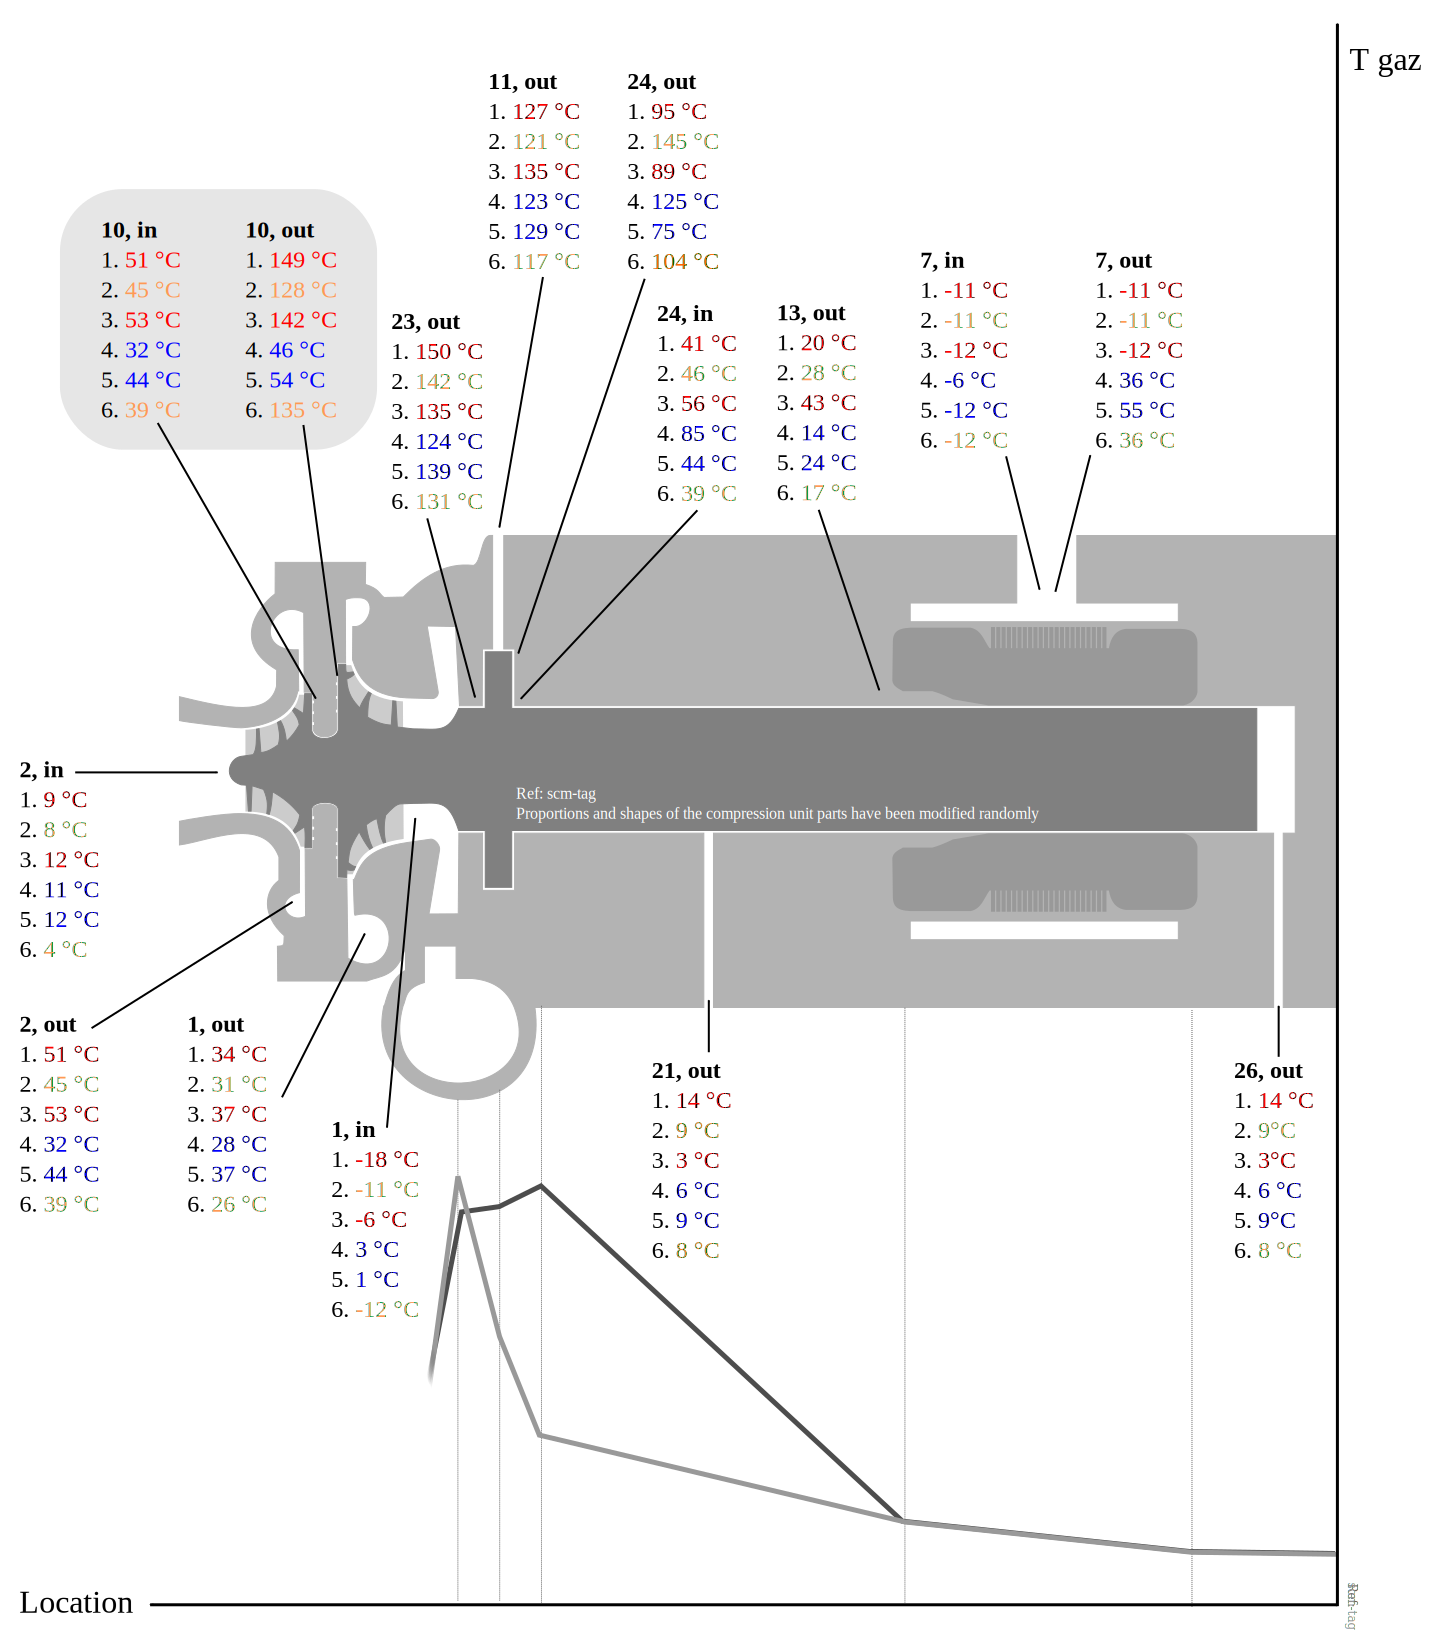
\includegraphics[width=1.0\textwidth]{cp105-awp-expT}
  \caption[Gas temperatures inside the compression unit]{Gas
    temperatures inside the compression unit. The temperature values
    are colored according to the level of gas outlet temperature in
    the labyrinth seal (outlet of component \#10). The lines of
    numbers in red have high labyrinth seal outlet temperatures, while
    the lines of numbers in orange have moderate outlet temperatures,
    and the lines of numbers in blue have low outlet temperatures. The
    temperature profiles at the bottom of the picture illustrate
    qualitatively the 2 types of profiles observed.}
  \label{fig:awp-cp-unit-gas-T}
\end{figure}


\subsubsection{Assumptions}
\label{sec:awp-laby-seal-hot-gas-assumptions}


\paragraph{Location of the hottest point:}

The results of the solving of the model for each of the stable \OP{},
summarized on \cref{fig:awp-cp-unit-gas-T}, let assume that the
location of the hottest point of the shaft is in the axial bearing
area. In the \OP{} \#1, \#3, \#5, and \#6, it seems to be between the
first stage impeller and the axial bearing. In the \OP{} \#2, and \#4,
it seems to be just at the location of the axial bearing side where
the gas stream flows reversely. This situation comes probably from the
lack of available data to constrain the model proposed in
\cref{sec:awp-model}. Indeed, minimums of the objective function can
currently be observed with more than one flow temperatures and heat
exchange, close to the axial bearing: the temperature peak can be
before or after the axial bearing without making a significant
difference in term of objective function. This situation occurs
because no mass or energy rates and no temperatures are known in this
area. Consequently, as soon as the global balances with the group of
components [\#11, \#12, \#23, \#24] are respected, it makes no
difference for the objective function and it exists more than one
configuration that satisfy the balances. This uncertainty about the
gas thermal profile could be solved easily by introducing a more
detailed thermal monitoring of the compression unit and its flows, as
it would allow to add more constraints in the model objective
function.

\paragraph{Gradient of temperature along the shaft:}

The temperatures observed through the solving of the \AWP{} model let
think that the shaft axial thermal gradient is quite strong close to
the bearings area. It could be that the shaft temperature is a lot
higher when the rotor speed is above 160 krpm as a result from
increased windage and parasitic electro-mechanical losses. Perhaps the
shaft temperature, between the impellers and the axial bearing, is a
function of the rotor speed. The shape of this function could be
exponential toward the rotor speed. This assumption can not be checked
in the frame of this work due to a lack of data. If this assumption
appears to be true, it may be that the axial bearing, traveled across
in the reversed way on one of its side, performs badly. It may be that
the relative location of the axial bearing in its gaps is not
appropriate, with this configuration of flow.


\paragraph{Improvement of the thermal design of the
  compression unit:}

Thermal management is an important area of the design of such
compression units, since the gaps between the parts are very small and
consequently, the dilatation phenomena have to be taken in account
very carefully. \citet[p.\,3]{Schiffmann-Favrat-2010b} state that the
thermal design and management of the compression unit is very
important to reach a good performance of the device and the integrated
multi-objective design method they propose takes the thermal
management into account through a lumped parameter approach. The unit
has been designed to sustain such high temperatures, but with the idea
in mind that the refrigerant used in the heat pump circuits would be
cleared from every trace of lubricant oil. Reaching such high
temperatures could create troubles due to the lubricant pollution
observed in the heat pump circuits\footnotep{The lubricant oil
  pollution issue is detailed in
  \cpref{sec:awp-issue-oil+corrosion}.}. Indeed, the synthetic
lubricant oil, heated up to those temperatures, might start to
deteriorate. The degradation of the lubricant oil creates
uncondensable gases which decrease the heat pump performance, as
those uncondensable gases are pumped in the cycle by the compression
stage without transferring heat energy efficiently from the evaporator
to the condenser.

\subsubsection{Scenarios to test in future work}
\label{sec:awp-laby-seal-hot-gas-next}

\paragraph{Improved thermal management of the unit:}

In 2013, \citet[p.\,1--2]{schiffmann-2013a} highlights the importance
of the thermal management in small scale radial compressors. He shows
that the gas bearings losses increase in proportion when the shaft
power decreases \citep[p.\,1 \& fig.\,1 p.\,2]{schiffmann-2013a} and
proposes design guidelines to decrease significantly the bearing
losses \citep[tab. 4 p.\,6]{schiffmann-2013a}. Consequently, a first
improvement would be to use bearings geometries which generate less
windage losses. It could also be possible to decrease the pressure
drop of the filter on the gas bearings aeration circuit, for example
by expanding its surface or set some of them in parallel, in order to
increase the mass flow rate in this aeration circuit. This increase
would result in a better heat dissipation in the unit. The shaft could
also maybe be redesigned in order to offer more surface to the
aeration flow, which would result in a better heat dissipation.

Moreover, having such a dissipation of energy in the axial bearing
area implies a high temperature of the impeller, and especially of the
first stage impeller. Part of the heat energy given to the impellers
is dissipated in the gas being compressed and this consequently
decrease the isentropic efficiency of the compression stages. In the
same spirit, the leak mass flow rate from the compression second stage
outlet to the first stage outlet, and the heat exchange happening
inside the seal, imply that the first compression stage isentropic
efficiency appears quite low ($\eta_{cp1,s,ext}$ in
\cref{tab:awp-cp-unit-isentropic-cdtns}). In fact, the first
compression stage isentropic efficiency is quite high ($\eta_{cp1,s}$
in \cref{tab:awp-cp-unit-isentropic-cdtns}), but is decreased a lot by
the leakage and the heat exchange. Those phenomena decrease the
efficiency of the compression unit, and consequently, the efficiency
of the whole heat pump cycle.

\paragraph{Correlation of the thermal profile with the rotor speed:}

So far, no direct correlation could be found between the energy rate
flowing from the shaft to the impellers $\dotQ{11}{1}$ and the
labyrinth seal (component \#10) outlet temperature $T_{10,\,out}$. It
would be interesting to to study the behavior of the labyrinth seal
more thoroughly. It may be that the design of the seal is not
appropriate to the conditions in the cycle, which would explain at
least partly the huge leaks observed between the two compression
stages. Those leaks are detailed in
\cref{tab:awp-cp-unit-isentropic-cdtns} with the mass flow rate
$\dotM{10}{25}$.

\subsection{Mixing and separating gas and liquid in the
  economizer:}
\label{sec:awp-issue-eco-separation}

\Cref{fig:awp-eco-gas-liq-sep-1-to-5} shows the different versions of
the economizer gas/liquid separation
parts. \Cref{fig:awp-eco-flow-rates} illustrates the separation
issues:

\begin{itemize}
\item The liquid is sucked up with a rotative gas flow bringing some
  of the liquid phase at the second stage compressor inlet.
\item The incoming superheated gas from the first stage compressor is
  not mixed properly with the incoming saturated gas/liquid flow
  coming from the second stage expansion valve. The gas in the
  economizer stays slightly superheated.
\end{itemize}

Those separation and mixing issues have mostly been solved through
different versions of the economizer mixing part. This part has been
improved through the experiments. 5 successive versions have been
used. The final version, the version \#5, can be seen on
\cref{fig:awp-eco-gas-liq-sep-5} and allows a satisfactory gas/liquid
mixing, resulting in a gas stream with less than 2 degrees of
superheating leaving the economizer, and a satisfactory gas/liquid
separation, blocking the swirling liquid phase streaming up along the
walls of the economizer.

\subsection{Decreasing the performance by using a
  4-way valve}
\label{sec:awp-issue-4way}

\begin{figure}[htbp]
  \centering
  \subfloat[A-6.8/W31.3 -- Refrigeration diagram]
  {\label{fig:awp-A-6.8/W31.3-Ph}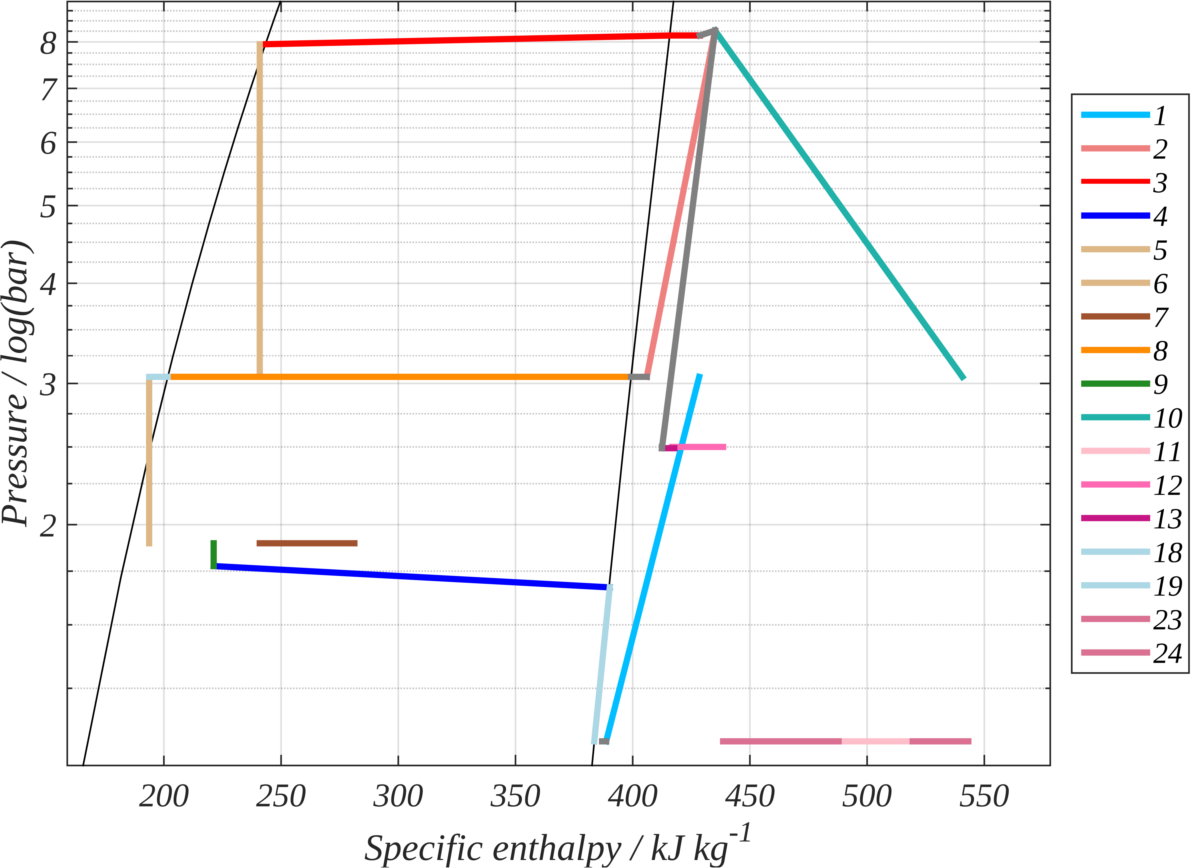
\includegraphics[height=50mm]{awp-Ph-20120511-132418-132718}}
  \hspace{1em}
  \subfloat[A-6.8/W31.3 -- Entropic diagram]
  {\label{fig:awp-A-6.8/W31.3-Ts}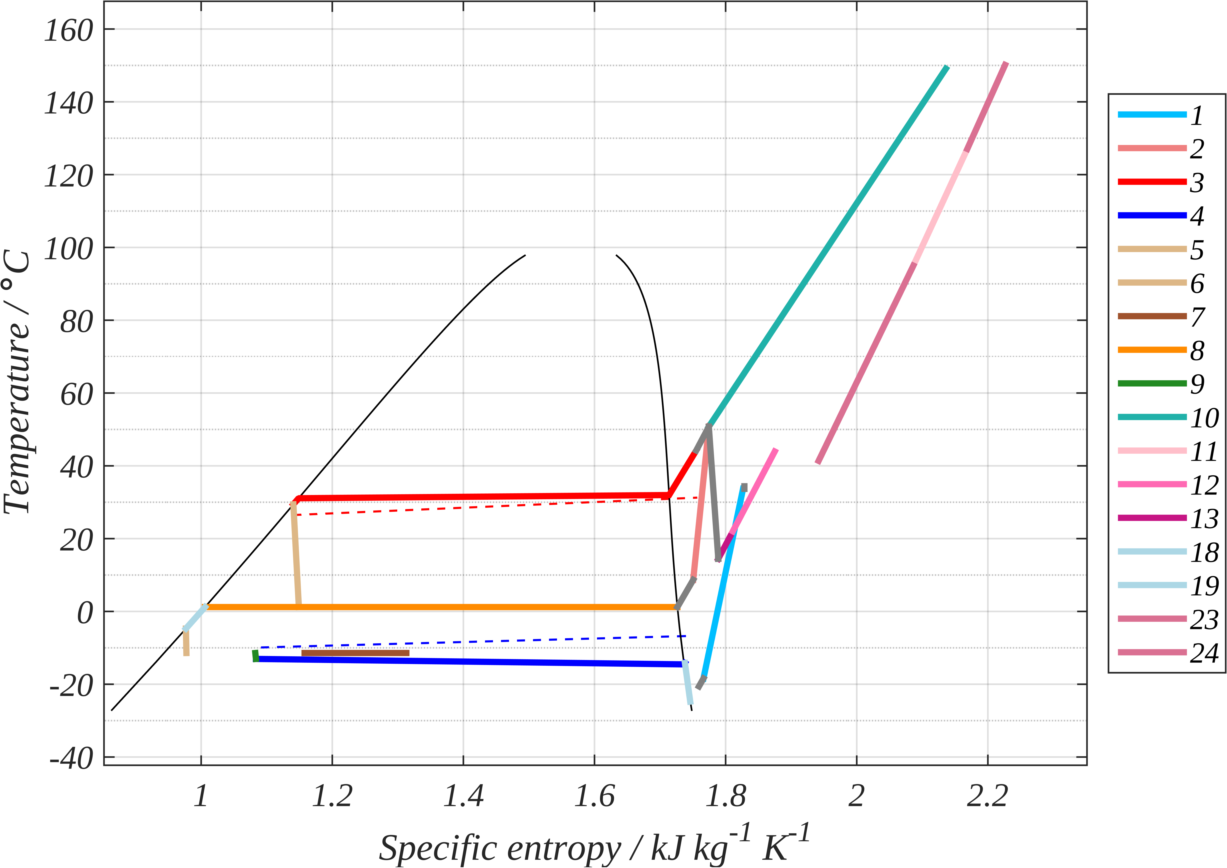
\includegraphics[height=50mm]{awp-Ts-20120511-132418-132718}}
  \\
  \subfloat[A-7.0/W32.3 -- Refrigeration diagram]
  {\label{fig:awp-A-7.0/W32.3-Ph}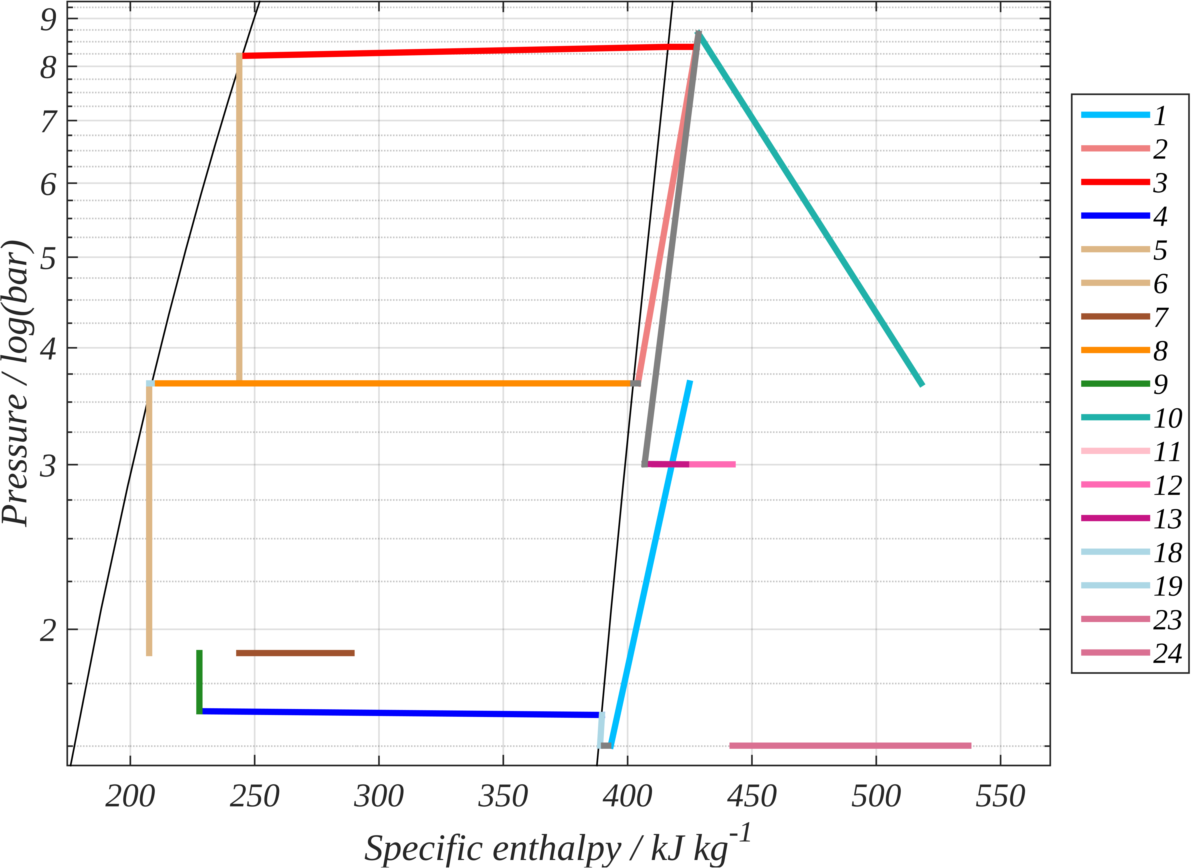
\includegraphics[height=50mm]{awp-Ph-20120531-103842-104143}}
  \hspace{1em}
  \subfloat[A-7.0/W32.3 -- Entropic diagram]
  {\label{fig:awp-A-7.0/W32.3-Ts}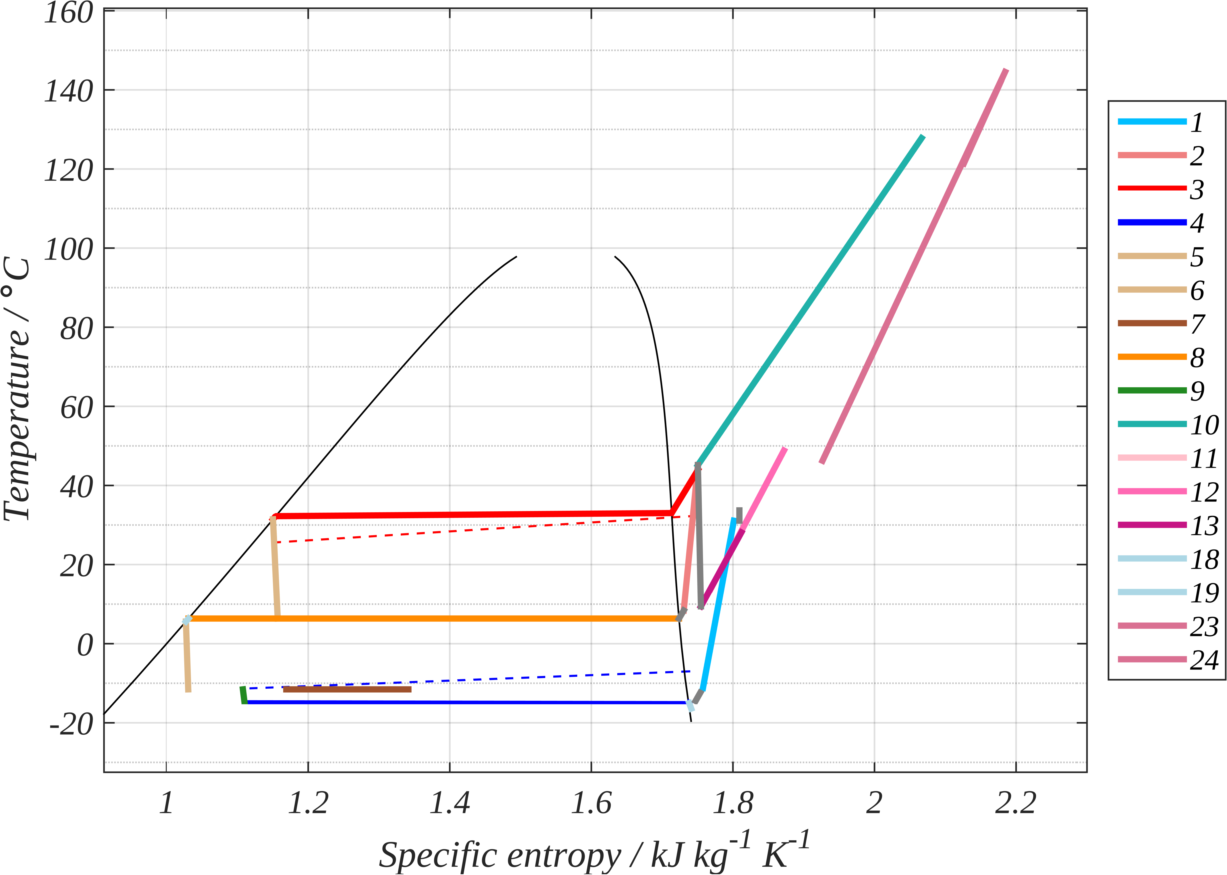
\includegraphics[height=50mm]{awp-Ts-20120531-103842-104143}}
  \caption[A-6.8/W31.3 \& A-7.0/W32.3 -- Thermodynamic diagrams with
  and without 4-way valve]{Thermodynamic diagrams with and without
    4-way valve. OP A-6.8/W31.3 has been recorded with the 4-way in
    the circuit while OP A-7.0/W32.3 has been recorded without the
    4-way valve.}
  \label{fig:awp-w-wo-4way-diagrams}
\end{figure}


The experiments were performed in heating mode. Some of those
experiments were performed with the normal circuit, through the 4-way
valve, and some were performed with a bypass around the 4-way
valve. \Cref{fig:awp-w-wo-4way-diagrams} shows the thermodynamic
diagrams for two similar \OP{}, with and without 4-way valve. The
\OP{} are similar in term of level of temperatures but there are some
significant differences, stressed out in
\cref{tab:awp-4way-differences}\footnotep{More details about those
  \OP{} are available in
  \cref{sec:awp-exp-details-A-6.8/W31.3,sec:awp-exp-details-A-7.0/W32.3}
  page~\pageref{sec:awp-exp-details-A-6.8/W31.3} and
  page~\pageref{sec:awp-exp-details-A-7.0/W32.3}.}. The pressure drop
difference on the vapor lines can be observed on the enthalpy diagram
and is detailed in \cref{tab:awp-4way-differences}. This example makes
the disadvantage of using a reversing 4-way valve very clear. Indeed,
the valve creates significant pressure drops before and after the
compression stages, decreasing the temperature difference potential of
the device, and generating exergy losses on vapor lines, which are the
worst location to create such losses.

\begin{table}[htbp]
  \begin{center}
    \footnotesize
    \begin{tabular}{lccccccc}
\toprule
OP & speed / krpm & $\dot{Y}_{cd}$ / \si{\kilo\watt} & $\dot{Y}_{ev}$ / \si{\kilo\watt} & $\dot{M}_{ev}$ / \si{\gram\per\second} & COP / - & $\Delta\,P_{4-way}$ / \si{bar}\\
\midrule
A-6.8/W31.3 & \num{170} & $ \num{7.4} \pm \num{0.2} $ & $ \num{4.3} \pm \num{4.3} $ & $ \num{32} \pm \num{2} $ & $ \num{2.19} \pm \num{2.19} $ & $ \num{0.597} \pm \num{0.597} $\\
A-7.0/W32.3 & \num{160} & $ \num{10.5} \pm \num{0.2} $ & $ \num{7.1} \pm \num{0.2} $ & $ \num{37.1} \pm \num{0.9} $ & $ \num{2.69} \pm \num{2.69} $ & $ \num{0.118} \pm \num{0.118} $\\
\bottomrule
\end{tabular}

  \end{center}
  \caption{OP comparison with and without 4-way valve}
  \label{tab:awp-4way-differences}
\end{table}


\subsection{Poor exergy efficiency of the evaporator
  and fluids maldistribution}
\label{sec:awp-issue-reducing-oh}

Maldistribution of the refrigerant and/or of the air in the evaporator
channels has been observed during the experiments. Indeed,
superheating values at the outlet of each evaporator channel vary a
lot, as illustrated
\cref{fig:awp-sh-col-distrib-profile-without-plate}. Difference of
superheat at the outlet of the evaporator circuits can be as high as
8\si{\kelvin}. Consequently, in order to get no liquid phase at the
outlet of the evaporator, high overall superheat values at the inlet
of the first stage compressor had to be imposed. The situation
observed when trying to decrease the superheat value is a good example
of the phenomenon observed by \citet{chen-yezheng-2002a}: indeed, the
superheat may decrease suddenly when it goes down below a certain
value, even if the opening of expansion valve is not changed in the
process. If that amount of superheat was decreased below
4\si{\degreeCelsius}, as illustrated on
\cref{fig:awp-sh-too-low-ev-sh-without-plate}, some liquid was
starting to flow into the first stage separator. Indeed, the liquid
and gas were not mixing together properly after the collector, and a
residual liquid flow was present even with some degrees of overall
superheat in the gas flow.

\begin{figure}[htbp]
  \centering
  \subfloat[Temperatures per circuit, without plate]
  {\label{fig:awp-sh-too-low-ev-T-without-plate}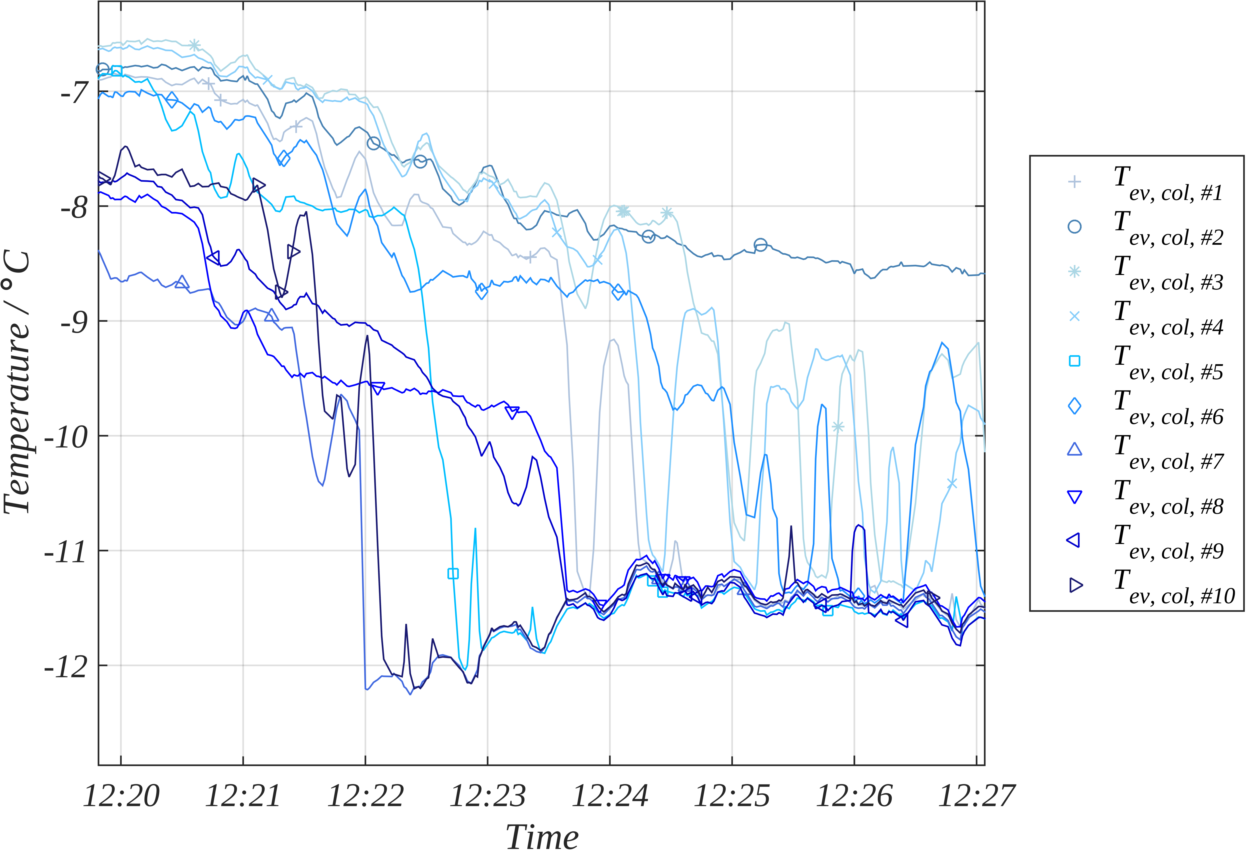
\includegraphics[width=0.45\textwidth]{awp-sh-too-low-ev-T-without-plate}}
  \hspace{1em}
  \subfloat[Temperatures per circuit, with plate]
  {\label{fig:awp-sh-too-low-ev-T-with-plate}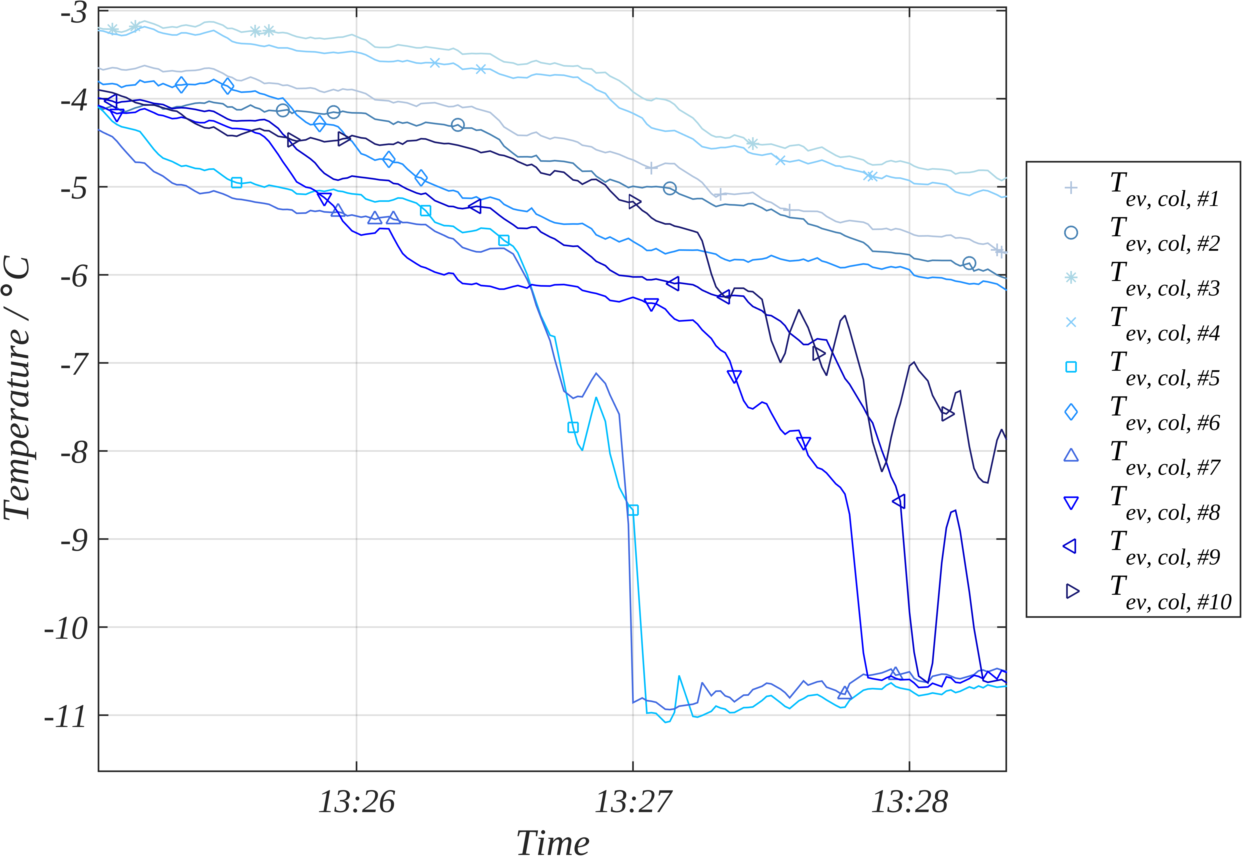
\includegraphics[width=0.45\textwidth]{awp-sh-too-low-ev-T-with-plate}}
  \\
  \subfloat[Superheating per circuit, without plate]
  {\label{fig:awp-sh-too-low-ev-sh-without-plate}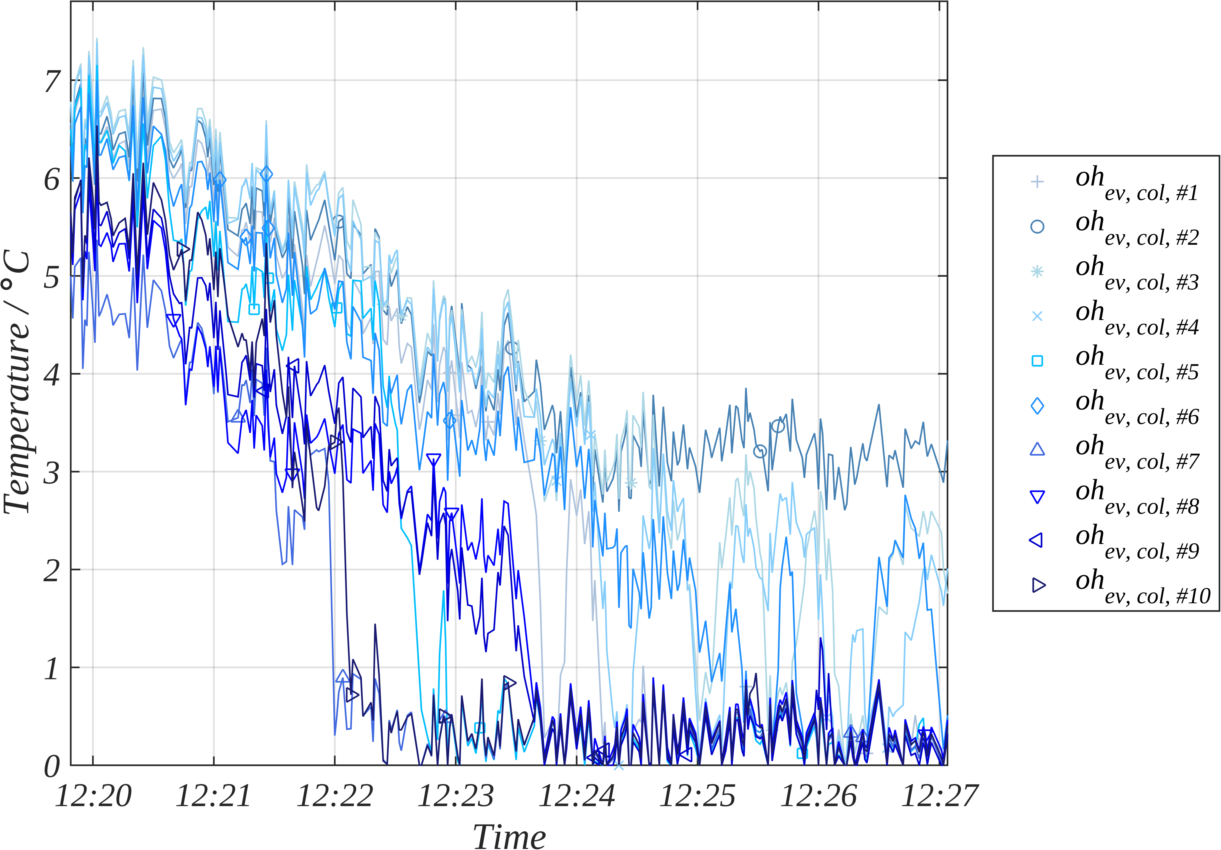
\includegraphics[width=0.45\textwidth]{awp-sh-too-low-ev-sh-without-plate}}
  \hspace{1em}
  \subfloat[Superheating per circuit, with plate]
  {\label{fig:awp-sh-too-low-ev-sh-with-plate}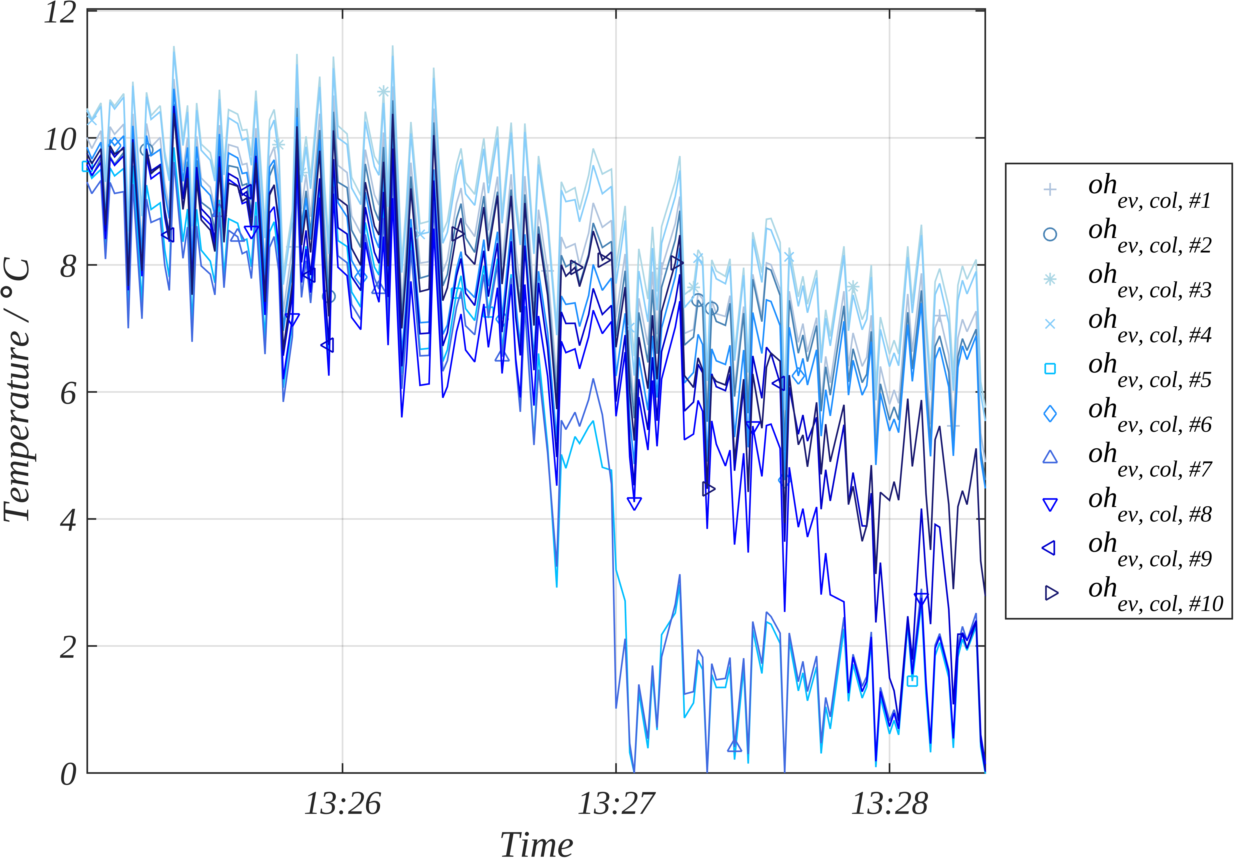
\includegraphics[width=0.45\textwidth]{awp-sh-too-low-ev-sh-with-plate}}\\
  \hspace{0.5em}
  \subfloat[Typical superheating profile, without plate]
  {\label{fig:awp-sh-col-distrib-profile-without-plate}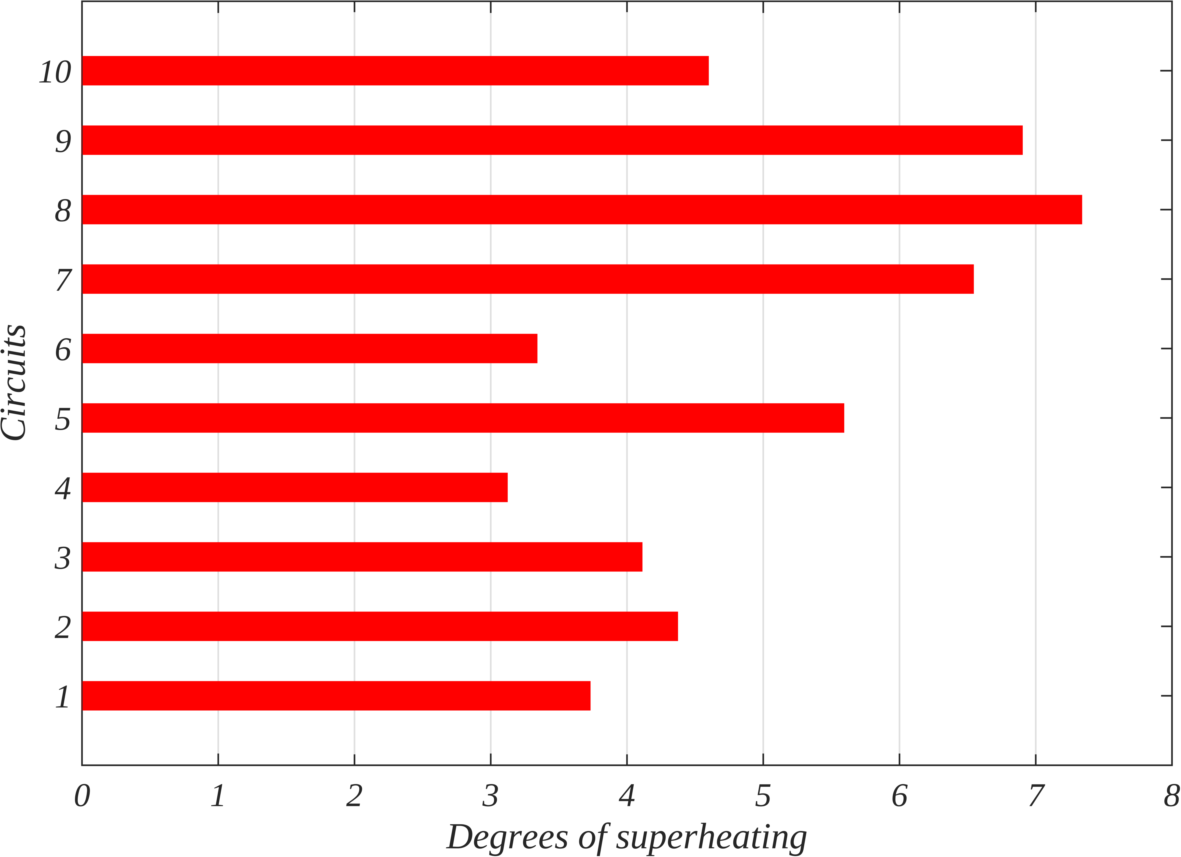
\includegraphics[width=0.35\textwidth]{awp-sh-col-distrib-profile-without-plate}}
  \hspace{5.8em}
  \subfloat[Typical superheating profile, with plate]
  {\label{fig:awp-sh-col-distrib-profile-with-plate}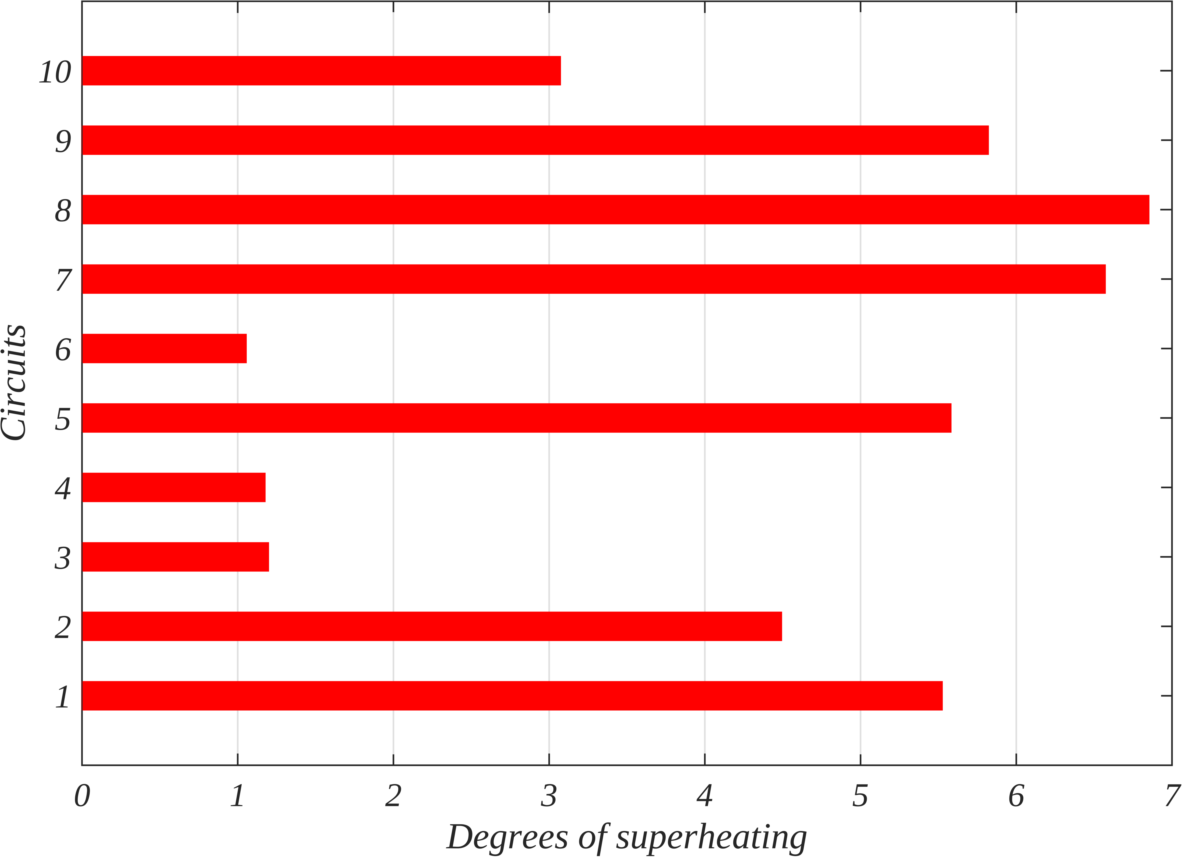
\includegraphics[width=0.35\textwidth]{awp-sh-col-distrib-profile-with-plate}}
  \hspace{5em}
  \caption{Refrigerant and air flow maldistribution in the evaporator}
  \label{fig:awp-maldistribution}
\end{figure}


The maldistribution observed in the refrigerant flow is caused by 2
factors:

\begin{itemize}
\item a non-ideal distribution of the liquid/gas flow coming from the
  lower stage expansion valve, implying that the distribution
  capillaries were not receiving the same mass flow rate and/or the
  same vapor fraction in the flow.
\item a non-ideal distribution of the air flow in the air ducting
  implying uneven speed profiles in the evaporator section. According
  to the location of the fan in the air flow, upper channels are
  exposed to a higher air mass flow rate. Clearly, the design of this
  air ducting emphasizes on compactness, not on effectiveness of the
  heat exchange.
\end{itemize}

None of these two factors could be quantified and studied in
depth. The problem seems to come more from the air ducting than from
the refrigerant distributor, in the experimenter's opinion. In an
attempt to decrease the air flow maldistribution phenomena, a plate
drilled with holes located in front of the evaporator circuits with
the lower superheat values was added 5cm away from the fins, upstream
to the air ducting inlet. The experiments performed after May
$11^{\text{th}}$ 2012 have been performed with this plate fixed
upstream to the air ducting inlet. As illustrated in
\cref{fig:awp-sh-col-distrib-profile-with-plate}, this attempt was a
failure. It even had the tendency to move the average overall
superheat value necessary to ensure the presence of gas only at the
first stage separator to a value increased by about
2\si{\kelvin}. The use of such plate would have been a
temporary solution, in any case, as the plate added a significant
pressure drop in the air flow, and consequently, increasing the
fan energy consumption.

\begin{figure}[htbp]
  \centering
  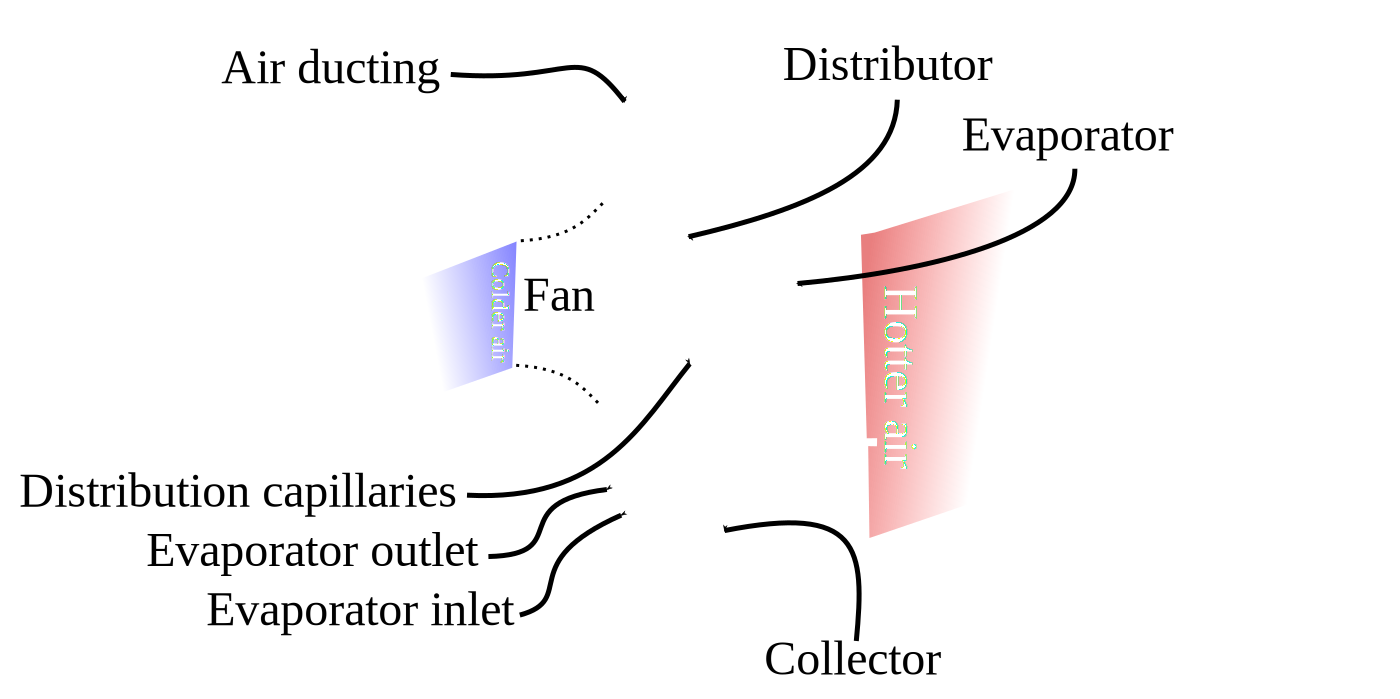
\includegraphics[width=15cm]{awp-airducting-commented}
  \caption{Air ducting with the fan and the fin-and-tube evaporator}
  \label{fig:awp-air-channel}
\end{figure}

It is possible that the control issue described in
\cref{sec:awp-issue-control} has an influence on the maldistribution
issue, as the refrigerant flow in the evaporator was controlled in an
attempt to get enough superheating at the first compression stage, but
the demonstration performed in \cref{sec:awp-issue-control} shows that
the mass flow rate in the first stage heat pump circuit is a function
of the second stage heat pump circuit mass flow rate and not a value
chosen independently using the first stage expansion valve. Those
elements are detailed further in \cref{sec:awp-issue-control}.

\subsection{Poor exergy efficiency of the subcooler}
\label{sec:awp-low-etaII-sc}

The exergy efficiency of the subcooler $\eta_{sc}$ is defined in
\cref{eq:eta_sc}, p.~\pageref{eq:eta_sc}, and is particularly low. As
detailed in \cref{tab:awp-performances-summary}, $\eta_{sc}$ ranges
from 0.4\% to 3\%. The low performance is the result of a poor
design of the heat exchanger\footnotep{This heat exchanger design is
  detailed in \cpref{sec:awp-subcooler-details}.}, a high temperature
difference between the fluids, and a significant difference of flow
rate between the two streams, as illustrated in
\cref{fig:awp-exp-analysis-model} and \cref{eq:sc-mf},
p.~\pageref{eq:sc-mf}. As it can be seen on
\cref{fig:awp-layout-model-numbers}, the location of the temperature
sensors were also not ideal to quantify accurately this efficiency.

\section{Control issues}
\label{sec:awp-control-issues}

Control issues are related to structural deficiencies and to design
mistakes of the prototype or of the compression unit. As the
prototypes have not been extensively tested, the control strategies
offered in this section and the issues encountered remain poorly
documented. They are mainly a testimony of the experimenter's
experience.

\subsection{Procedure to start the cycle}
\label{sec:awp-proc-start}

As the compression unit is a radial compression machine, it needs to
be equipped with a compressors bypass system. Indeed, in order to
start the installation away from the surge domain, the characteristics
of the circuit needs to be contained into the operation range of the
compressors\footnotep{See \cpref{fig:bypass-in-maps} for an
  illustration of the bypass circuits flow characteristics in
  compression maps.}, represented by the inner surface of the
compressors maps. In heat pump applications, starting an installation
without bypass systems is likely to yield operation outside of the
radial compressor map, at least during the start-up time. Indeed, in
domestic heat pumps applications the temperature levels of the sources
can not be changed by the heat pump control, as those temperature
levels are imposed by the environment and by the house. Having defined
temperature levels imposes defined pressure levels at the main heat
exchangers and consequently, at the inlet of the first compression
stage and at the outlet of the second compression stage. For a radial
compressor, starting up with no mass flow rate and an already existing
pressure ratio would result in surge which might damage the
compressor. In order to avoid this situation, the compression unit is
started within a bypass circuit which provides flow resistance
characteristics compliant with the compressor maps. Namely, this
implies that the characteristics of the bypass circuits always fits
into the compressors maps, as illustrated \cref{fig:bypass-in-maps}.

The implemented procedure to start the heat pump prototype is:

\begin{enumerate}
\item Liquid is present at the bottom of the condenser, at the bottom
  of the economizer, and at the inlets of the expansion valves,
  ideally. As the \AWP{} have two separated bypass circuits (one per
  compression stage), it is possible to start with no liquid in the
  economizer, as it was the case in most of the experiments
  performed. In that case, the upper part of the cycle is started
  first while the first compression stage is being bypassed. When
  liquid arrives in the economizer, the lower part of the cycle is
  also started.
\item The compression unit is started at 60 krpm with fully open
  bypass circuits and fully closed expansion valves.
\item The second stage bypass circuit is closed and the second stage
  expansion valve is open, but not much. A typical value is 20\% of
  opening for this valve in this situation. As the bypass circuits are
  made of a manual needle valve and a solenoid valve, in the \AWP{},
  the upper part of the cycle switches from the bypass circuit to the
  main circuit instantly, inducing an instantaneous change of pressure
  ratio and mass flow rate in the compression unit. This might induce
  surge at the second stage impeller, if pressure ratio is already too
  high between the economizer (which is approximately at the climate
  chamber temperature and consequently probably at a low pressure
  level as the room temperature might be low) and the condenser (which
  might be at a temperature much higher as the house space heating
  water flows into it). In that case, the compression unit rotor speed
  is increased until the second compression stage leaves the surge
  domain. This happens below 120 krpm in the tested cases.
\item As the upper part of the heat pump cycle stabilizes, saturated
  liquid and gas enters the economizer. The second stage expansion
  valve is set to an opening small enough to increase the pressure
  level at the condenser and get some degrees of subcooling at the
  condenser outlet.
\item The first stage expansion valve is open with a small opening and
  the first compression stage bypass circuit is closed. Typically, the
  first compression stage enters the surge domain as the pressure
  difference between the economizer and the evaporator is already not
  equal to zero anymore and no refrigerant flows yet through the
  valve, while some gas is being pumped in the evaporator. With no
  flow rate, the compression unit is not able to perform a pump down
  of the evaporator. This needs to be done gradually, and that is also
  why having a controllable bypass circuit has been favored for the
  \BWP{}. Leaving the surge domain is more difficult in this case,
  since this operation implies some increase of the compression unit
  rotation speed, some opening of the first stage expansion valve, and
  depends on the liquid brought at the economizer. If there is no
  liquid in the economizer, it is useless to open the first stage
  expansion valve further. Consequently, starting the lower part of
  the cycle heavily depends of the situation in the upper part of the
  cycle.
\end{enumerate}

With more experience with the setup, this procedure could be
automated. First, the control system could involve level control
devices, and then, with a good knowledge of the device dynamics,
control levels could be removed or kept at their minimal expression
(presence of liquid or not).

\subsection{Procedure to reverse the cycle}
\label{sec:awp-proc-reversing}

The procedure to reverse the cycle is detailed here. It has not been
properly tested as an inversion of the cycle happened only once and
with a low difference between the sources temperature levels.

\begin{enumerate}
\item The heat pump operates at a given \OP{}.
\item Both bypass circuits are open and expansion valves are closed.
\item The compression unit rotational speed is decreased to 120 krpm
  where the stiffness of the bearings is already good and the rotation
  speed reasonably lowered.
\item The reversing 4-way valve is activated. Liquid might flow from
  the condenser to the first stage separator.
\item The first stage bypass circuit is closed. The first stage
  expansion valve is open with a small opening. The goal is to get an
  opening big enough to stay away from the surge domain, but small
  enough to create a significant pressure ratio and decreasing this
  way the pressure in the separator. The second stage expansion valve
  is closed and the second stage bypass circuit is open. The liquid in
  the separator has to be evaporated before increasing the compression
  unit rotational speed too much, in order to prevent droplets and
  liquid suction into the first compression stage. The liquid
  evaporates with the combined action of the energy rate coming from
  the subcooler circuit and the decreasing of the pressure level in
  the evaporator, through the reduction of the first stage expansion
  valve opening.
\item When the liquid in the separator is evaporated, the compression
  unit rotational speed can be increased again.
\end{enumerate}

\subsection{Procedure to stop the cycle}
\label{sec:awp-proc-stop}

\paragraph{During experiments:}

During the experiments, the sources temperature levels difference was
gradually reduced in order to be below \num{10}\si{\kelvin}. The
compressor bypass circuits were open, and the compression unit
rotational speed was reduced to 120 krpm and then, the unit was
stopped.

\paragraph{Normal operation:}

Originally, the industrial partner had requested that the filter
included in component \#26 is bypassed by the activation of the
solenoid valve between components \#26 and \#21, in order to set the
pressure levels in the compression unit housing to the intermediate
pressure level before the compression unit deceleration reaches the
dangerous speed zone ranging between 80 krpm and 60
kprm\footnotep{\label{fnote:rot-danger-zone}See
  \cpref{sec:awp-P-balance} for more details about the dangerous
  rotational speed zone.}. This procedure was dangerous, since it
implied the bypass of the filter, which could imply the admission of
dusts of critical sizes inside the radial bearings
cavity (component \#12). Practically,
this procedure has been kept for emergency situations, which did not
occur often, so it is untested. The favored procedure was to lower the
temperature levels difference (reducing consequently the pressure
level differences, which was also reducing the efforts on the axial
gas bearing) and to simply stop the compression unit.

\paragraph{Emergency situations:}

In emergency situation, the procedure would be to open the solenoid
valve between components \#26 and \#21, and as the compression unit
starts to slow down, and in any case before the dangerous speed zone
is reached\cref{fnote:rot-danger-zone}, and to open the bypass
circuits while closing the expansion valves. When the compression unit
has stopped, the solenoid valve can be closed again. This procedure
has not been tested during the experimental campaign.


\subsection{Setting an appropriate gas bearings
  aeration circuit flow rate}
\label{sec:awp-issue-bearings-aeration}

Providing the needed gas flow to the gas bearings aeration circuit is
problematic. As described in \cref{sec:cp-intg-aeration}, the 0.5
\si{\micro\meter}-filter is by-far the main pressure drop of the
circuit, which means that the needle valve located before the filter
has a low authority on the circuit flow rate. In fact, the pressure
drop of the filter is too big for the pressure difference observed
between the high pressure zone and the low pressure zone, which
reduces the flow rate possible in the aeration circuit. Practically,
the 1.2 \si{\gram\per\second} measured during the tests could not be
increased significantly. Reducing the flow was also difficult, since
closing the manual needle valve had no consequence with the first
turns, then closing the valve was resulting very fast in a significant
decrease of the flow (the valve was indeed too big and had a low
authority on the flow, but a smaller valve would have decreased the
flow further more). The 0.5 \si{\micro\meter}-filter is necessary to
protect the set of bearings from small dusts that could block grooves
in the set of bearings. The dust-size range to filter here is 0.5 to 5
\si{\micro\meter}, which is the range of dangerous dust size for the
bearings. In order to decrease the filter pressure drop, increasing
the surface of the filter or mounting more filters in parallel would
have been valid solutions.


\subsection{Setting an appropriate motor cooling circuit
  flow rate}
\label{sec:awp-issue-motor-cooling}


\begin{figure}[htbp]
  \centering
  \subfloat[A-3.1/W29.5 -- Refrigeration diagram]
  {\label{fig:awp-A-3.1/W29.5-Ph}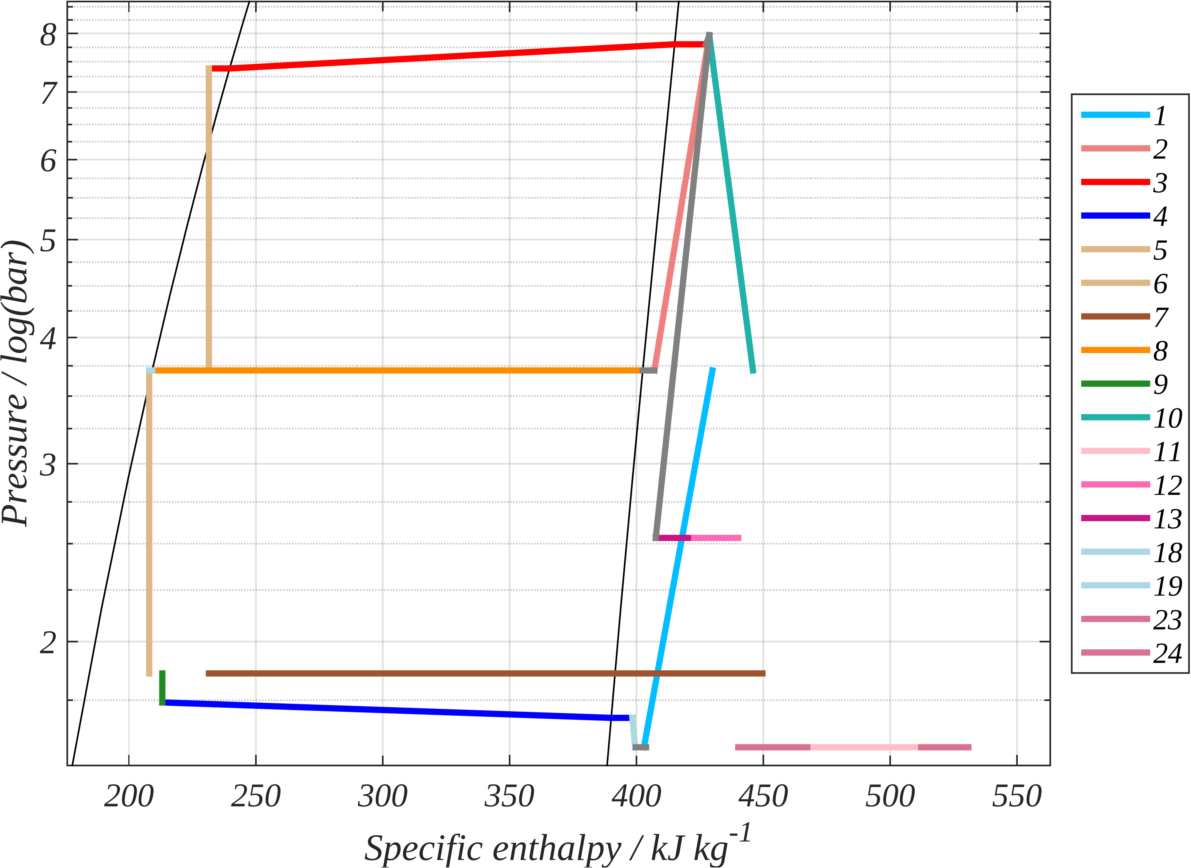
\includegraphics[height=50mm]{awp-Ph-20120525-130157-130457}}
  \hspace{1em}
  \subfloat[A-3.1/W29.5 -- Entropic diagram]
  {\label{fig:awp-A-3.1/W29.5-Ts}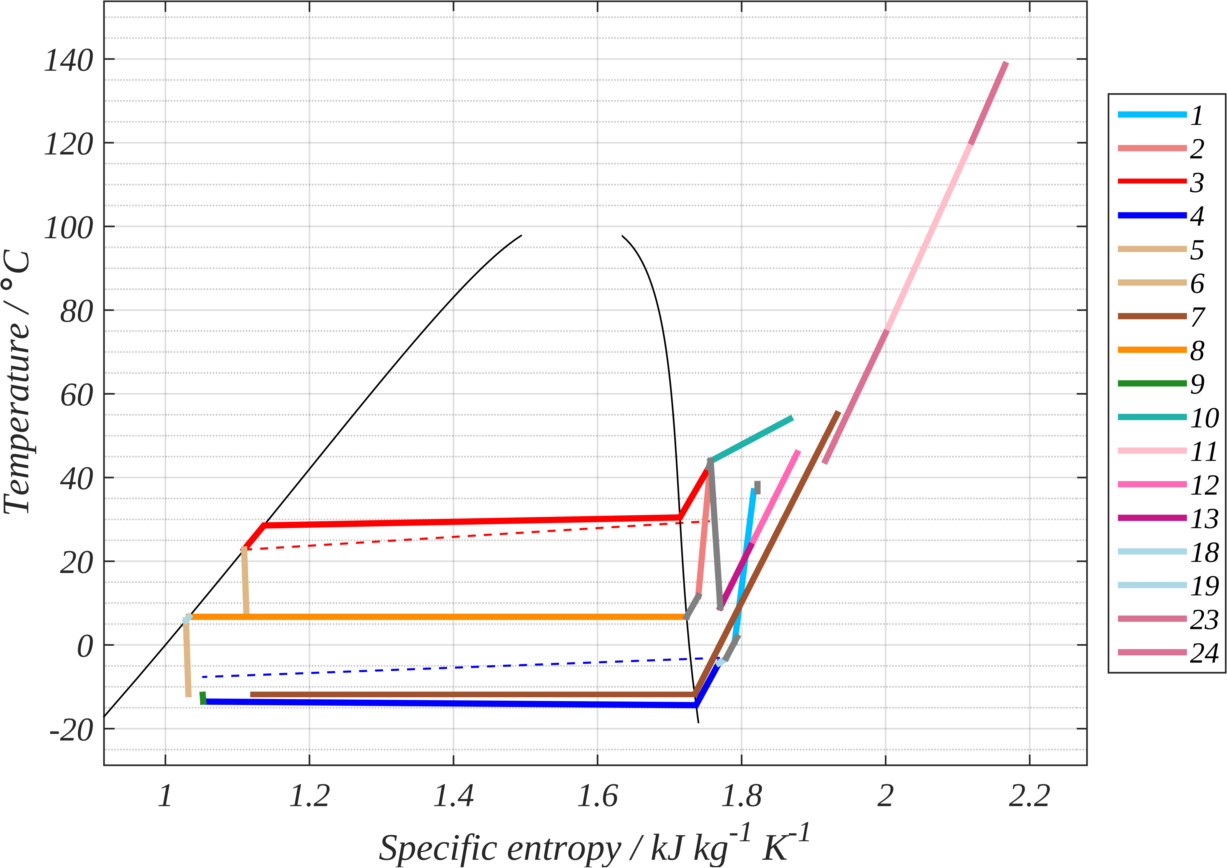
\includegraphics[height=50mm]{awp-Ts-20120525-130157-130457}}
  \\
  \subfloat[A-6.6/W22.1 -- Refrigeration diagram]
  {\label{fig:awp-A-6.6/W22.1-Ph}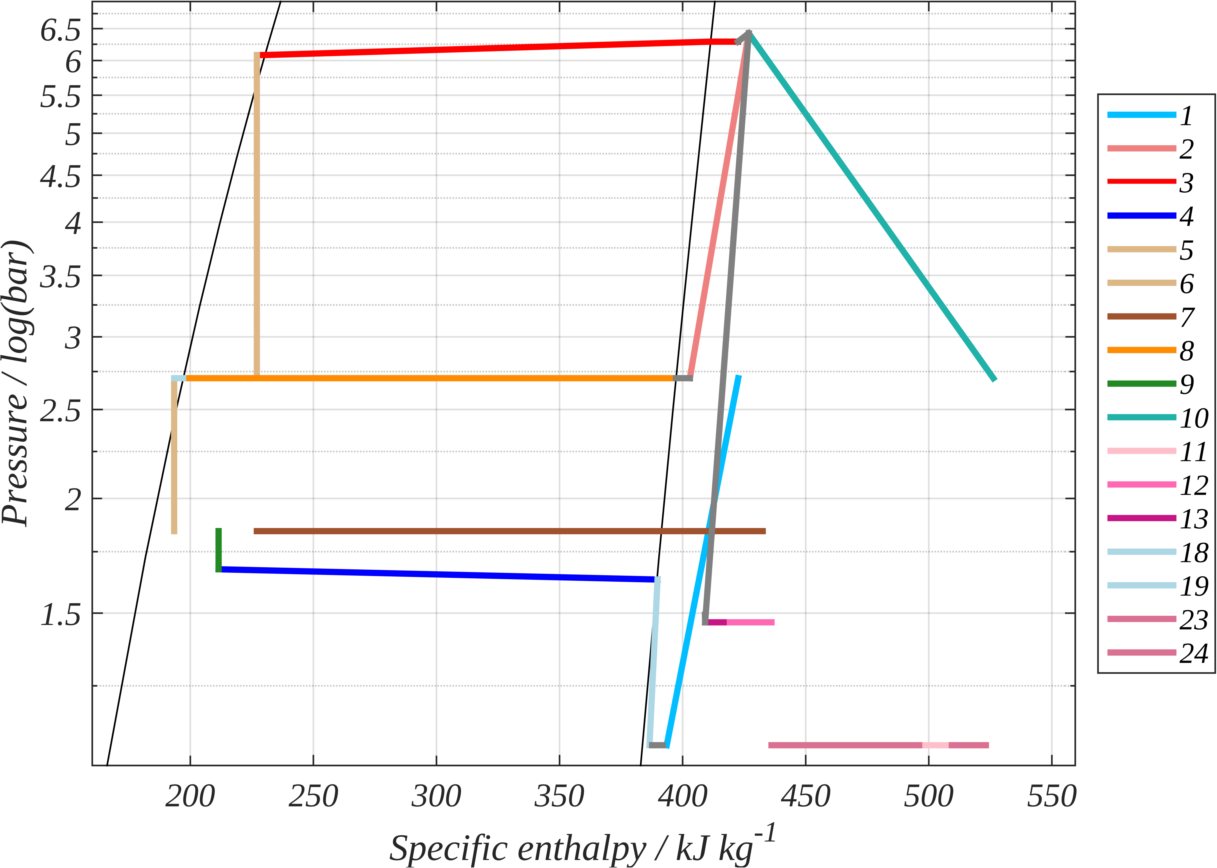
\includegraphics[height=50mm]{awp-Ph-20120511-123824-124126}}
  \hspace{1em}
  \subfloat[A-6.6/W22.1 -- Entropic diagram]
  {\label{fig:awp-A-6.6/W22.1-Ts}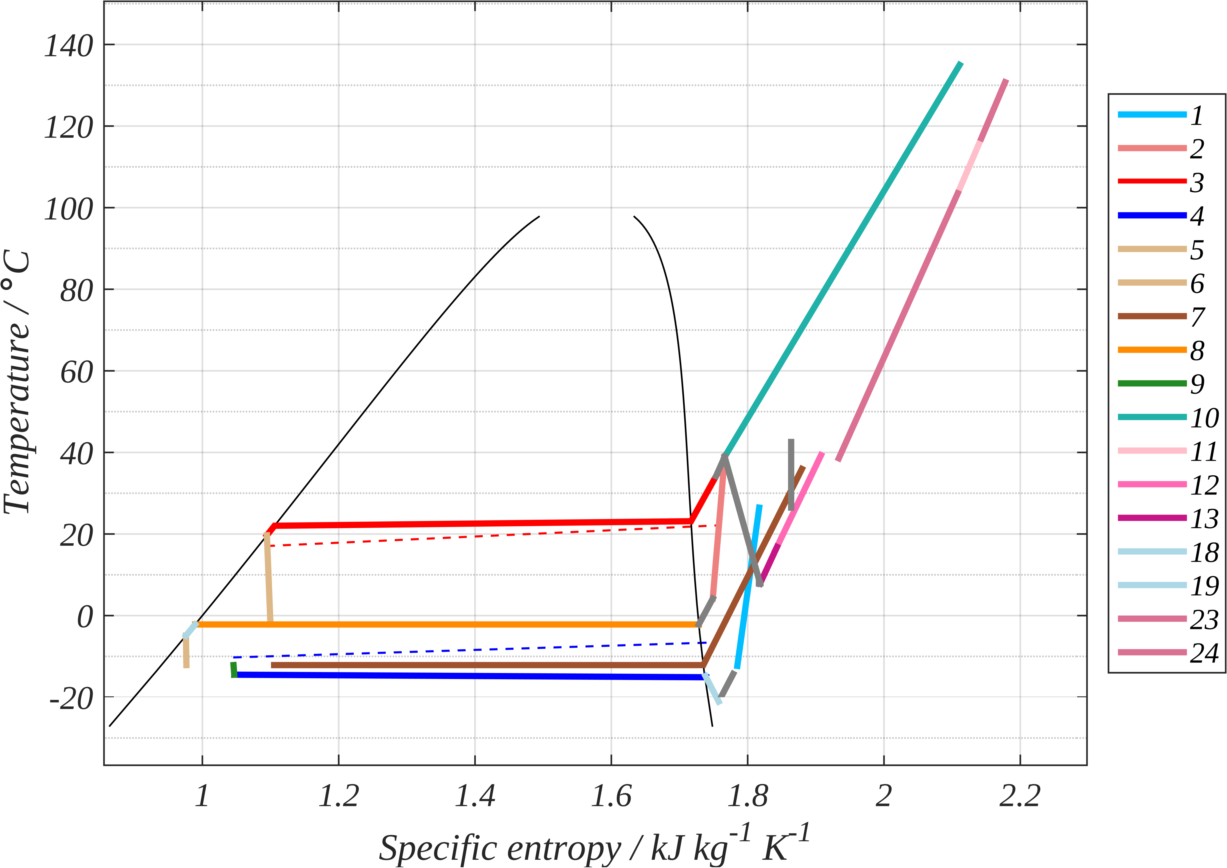
\includegraphics[height=50mm]{awp-Ts-20120511-123824-124126}}
  \caption[A-3.1/W29.5 \& A-6.6/W22.1 -- Thermodynamic
  diagrams]{A-3.1/W29.5 \& A-6.6/W22.1 -- Thermodynamic diagrams. The
    diagrams illustrate notably a too low mass flow rate in the motor
    cooling chamber, as the vapor quality at the outlet of the motor
    cooling circuit (component \#7) is too high. An other example of
    this situation can be observed for the OP A-0.5/W20.7 in
    \cref{fig:bwp-B8.0/W11.0-A-0.5/W20.7-diagrams}.}
  \label{fig:awp-too-high-motor-cooling-flow}
\end{figure}

\begin{figure}[htbp]
  \centering
    \subfloat[A-7.0/W35.6 -- Refrigeration diagram]
  {\label{fig:awp-A-7.0/W35.6-Ph}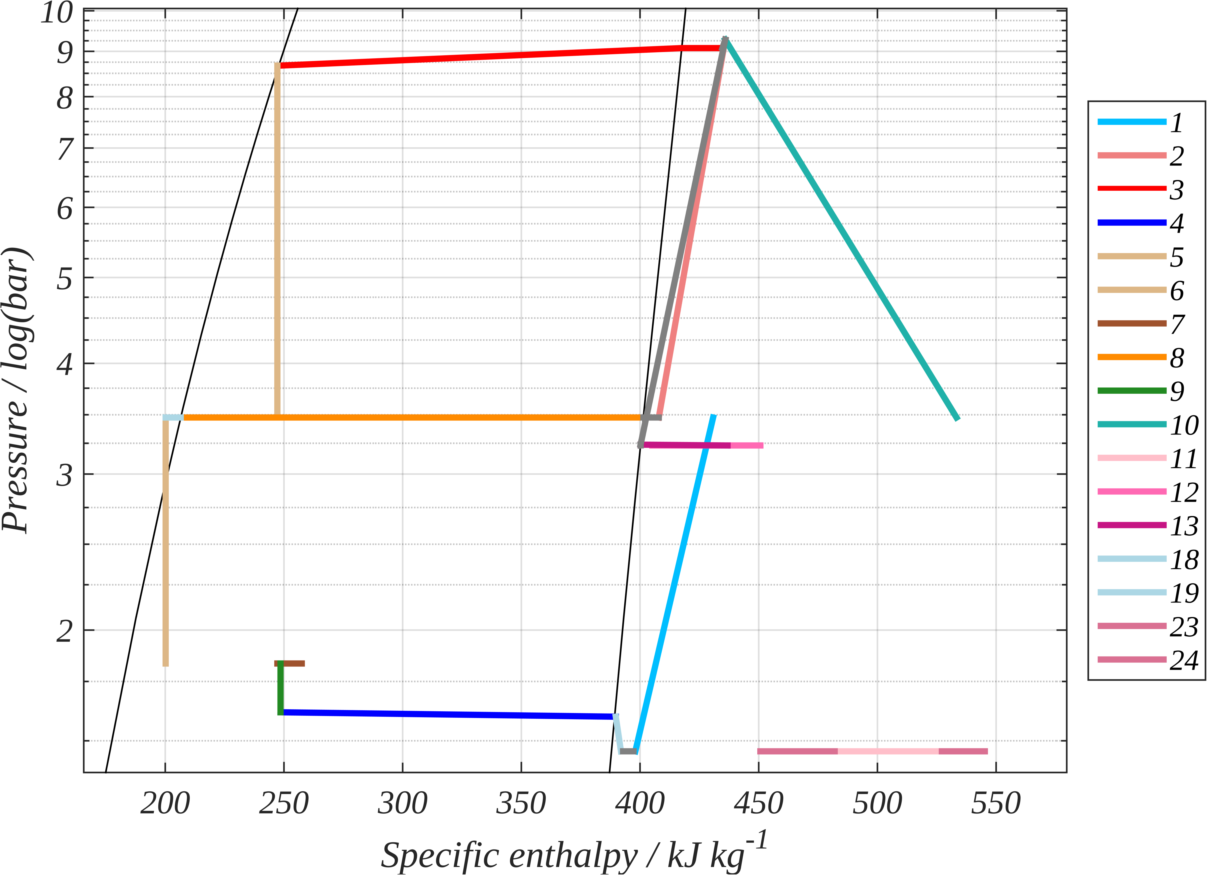
\includegraphics[height=50mm]{awp-Ph-20120525-150822-151122}}
  \hspace{1em}
  \subfloat[A-7.0/W35.6 -- Entropic diagram]
  {\label{fig:awp-A-7.0/W35.6-Ts}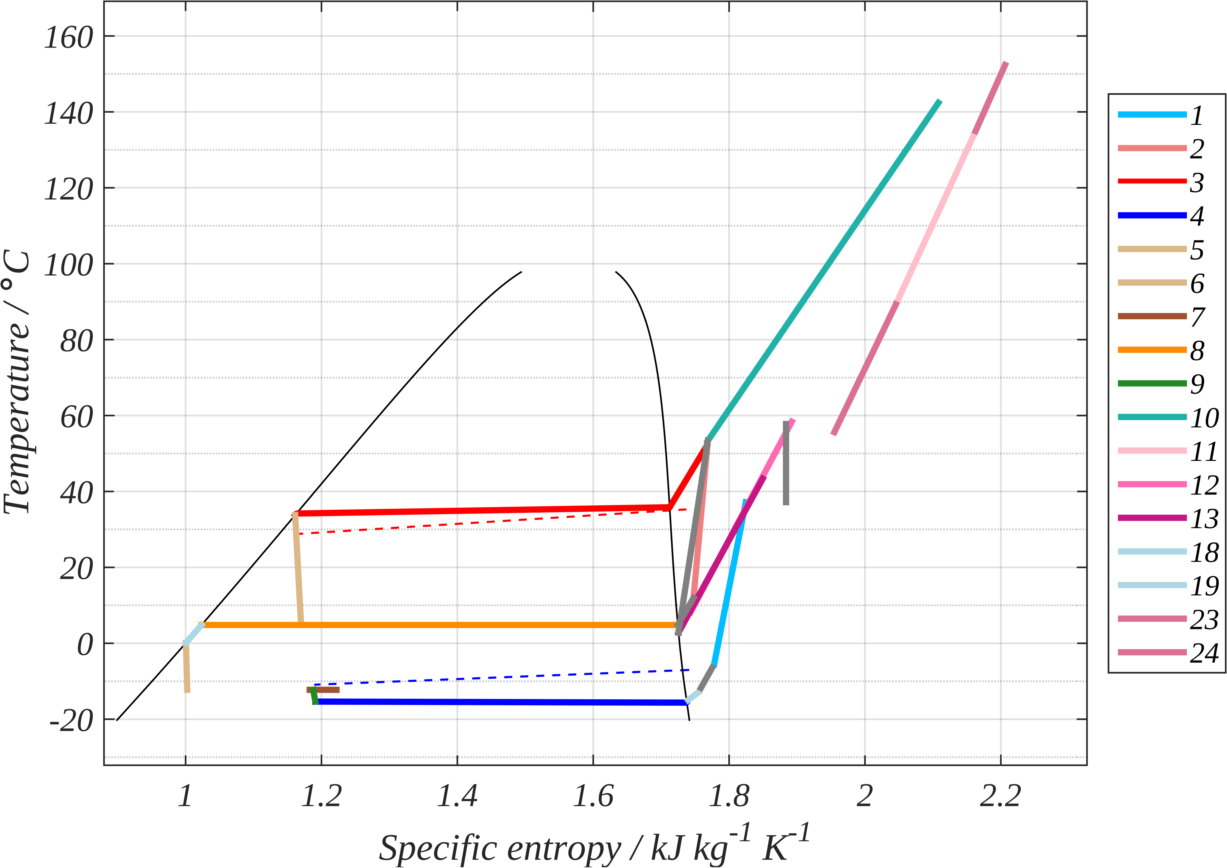
\includegraphics[height=50mm]{awp-Ts-20120525-150822-151122}}
  \caption[A-7.0/W35.6 -- Thermodynamic diagrams]{A-7.0/W35.6 --
    Thermodynamic diagrams. The diagrams illustrate notably a too high
    mass flow rate in the motor cooling chamber, as the vapor quality
    at the outlet of the motor cooling circuit (component \#7) is
    low. Others examples of this situation can be observed for the OP
    A-6.8/W31.3 and A-7.0/W32.3 in \cref{fig:awp-w-wo-4way-diagrams}.}
  \label{fig:awp-too-low-motor-cooling-flow}
\end{figure}

As it can be observed in the entropy diagrams in
\cref{chap:exp-details}, often, during the experiments, the flow in
the motor cooling chamber was not appropriate. Ideally, the flow of
refrigerant sent to the motor cooling circuit would be fully
evaporated. For \OP{} A-6.8/W31.3, A-7.0/W32.3 and A-7.0/W35.6, the
flow was too high, as the vapor quality at the outlet of the motor
cooling chamber was low. This phenomenon can be observed on the
diagrams in
\cref{fig:awp-too-high-motor-cooling-flow,fig:bwp-B8.0/W11.0-A-0.5/W20.7-diagrams}. In
the contrary, in \OP{} A-0.5/W20.7, A-3.1/W29.5, and A-6.6/W22.1, the
flow was too low and the refrigerant was leaving the motor cooling
chamber with too much superheat. This phenomenon can be observed in
the diagrams in
\cref{fig:awp-too-low-motor-cooling-flow,fig:awp-w-wo-4way-diagrams}. At
this flow regulation problem, is added the oil separation problem,
which is detailed in \cref{sec:awp-issue-oil+corrosion}. Indeed, in
the \AWP{}, the motor cooling chamber acts as a lubricant oil
separation device. The compression unit \textit{cp101}, after being
removed from one of the industrial partner installations which used
the same motor cooling system as for the one in the \AWP{}, was
partially filled with synthetic lubrication
oil. \Cref{fig:awp-motor-with-oil} illustrates how the motor cooling
chamber was probably performing with an effective cooling of the upper
part of the motor and a defective cooling of the lower part, mainly
surrounded by refrigerant liquid saturated of lubricant oil. Of
course, the presence of this oil significantly decreases the
performance of the motor cooling system, as the gap between the two
walls of the motor cooling chamber is small, and because there is no
circulation of the refrigerant around the motor. A defective motor
cooling system can result in unexpected deformations of the motor
parts, and especially of the shaft and can also result in an overheat
of those parts, damaging them heavily. The mounting of the magnets on
the shaft is also sensitive to overheat. Consequently, a flow boiling
motor cooling system might be a better option for the motor cooling
circuit until clean and lubricant-free refrigerant can be obtained and
guaranteed by the industry supply chain.

\begin{figure}[htbp]
  \centering
  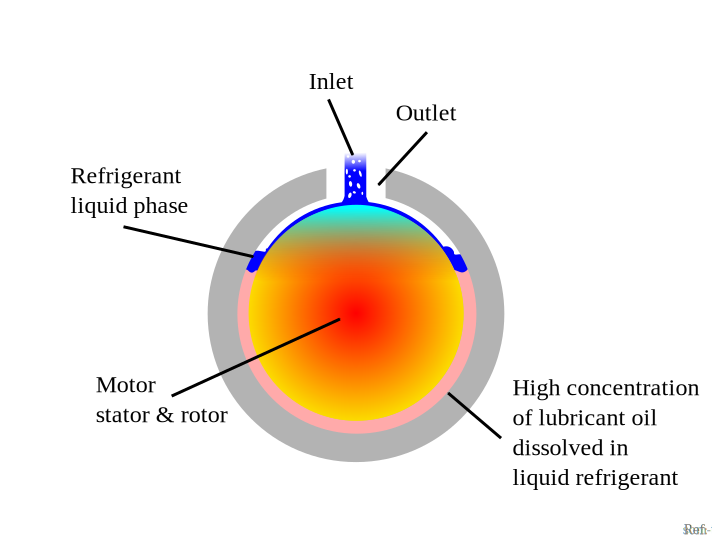
\includegraphics[width=10cm]{motor-cooling-with-oil-schematics}
  \caption[Schematic of the motor cooling chamber filled up with
  lubricant oil]{Schematics of the motor cooling chamber filled up
    with lubricant oil. The cooling down of the motor, symbolized
    qualitatively with the red to blue colors, is not isosymetric
    which could cause dilatation differences and a motor failure.}
  \label{fig:awp-motor-with-oil}
\end{figure}

\subsection{Controlling the heat pump to reach stable OP}
\label{sec:awp-issue-control}

\begin{itemize}
\item Absolute pressure in the economizer (component
  \#8)\index{economizer} was barely affected during the experiments by
  the settings of the prototype, including compressor speed and valves
  settings.
\item The subcooling value was stabilizing itself around an almost
  fixed value and was almost independent of the setting of the second
  stage expansion valve.
\end{itemize}

\begin{figure}[htbp]
  \centering
  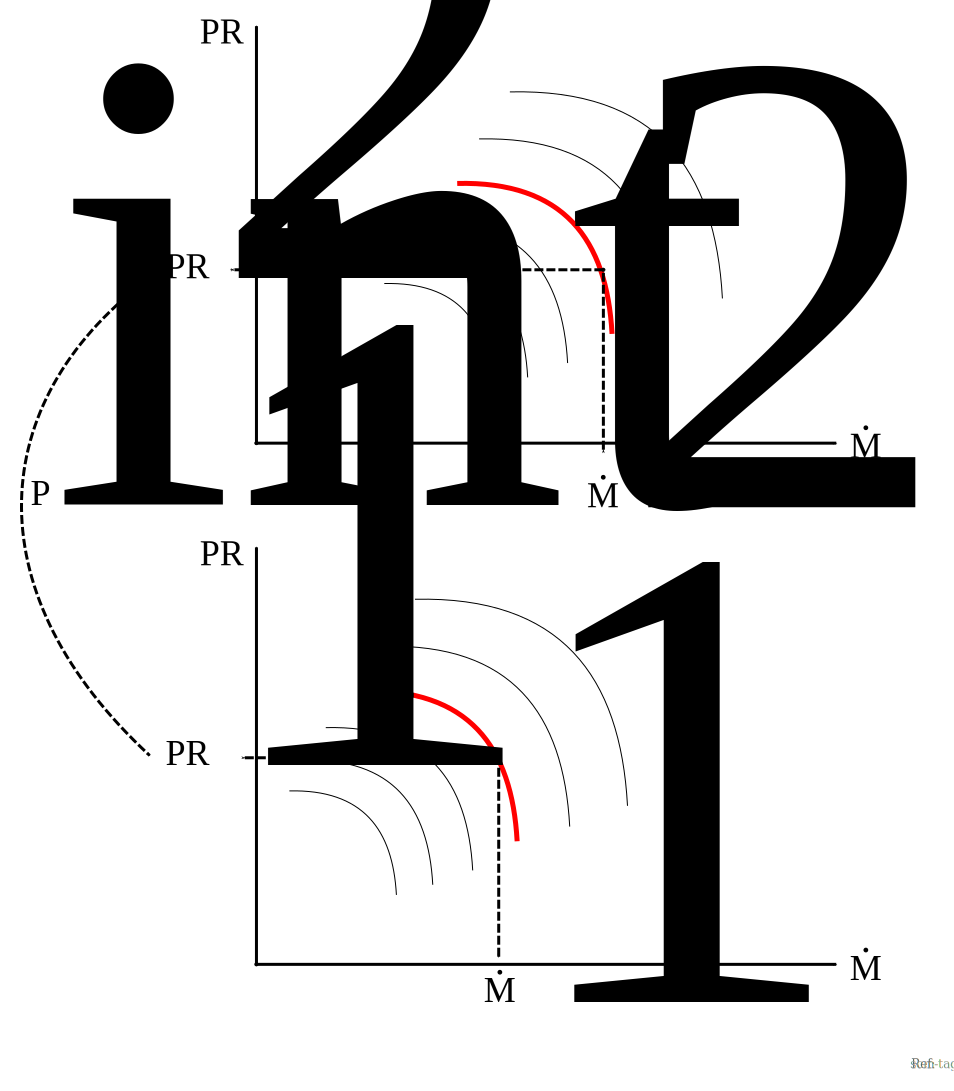
\includegraphics[width=11cm]{control-ppe-with-2cp}
  \caption[The flow rates of the compression stages are bound
  together]{The mass flow rates of the two compression stages are
    bound together through the pressure levels and compression unit
    current rotational speed. }
  \label{fig:awp-control-ppe-2cp}
\end{figure}

Those two phenomena are explained by the nature of the control system
needed for such a heat pump. If the economizer is perfectly insulated,
the intermediate pressure level is defined by the balance of the
economizer inlet and outlet mass flow rates and enthalpies. Being
external conditions, hot source inlet and outlet temperatures are
imposed. The second compression stage provides the heating service to
the house, so its mass flow rate and pressure level is set by the
external conditions. The intermediate pressure level and the choice of
the compressor rotation speed sets the first stage compressor mass
flow rate, as shown in \cref{fig:awp-control-ppe-2cp}. However, the
main function of the first stage expansion valve is to maintain an
overheating value at the first stage compressor inlet. So, the valve,
trying to reach the desired level of overheating, will influence the
first stage mass flow rate and the intermediate pressure level
together.  This will imply the setting of the second stage expansion
valve in order to maintain the second stage mass flow rate, needed to
perform the heating service (change of the intermediate pressure level
implies a change of the mass flow rate if there is no change of the
rotational speed). Consequently, the intermediate pressure level can
not be controlled independently and is a consequence of the choice of
the compression unit rotation speed and the setting of the valves. The
control system needs to control the valves and the rotation speed all
together. Designing such a control algorithm is foreseen as the only
way to control the heat pump in order to reach a stable \OP{} for
every external conditions. This explanation tends to prove that there
is one and only one setting of the valves and rotation speed that
allows to reach a given intermediate pressure level and overheating
value for given external conditions. Of course, this reasoning implies
that the two compressor maps provide a common working point where the
energy and mass balances on the economizer can be satisfied. During
the experiments, the sources temperatures and mass flow rate have been
modified to stabilize the \OP{}, as the heat pump was controlled
manually. Moreover, mass flow rates in the auxiliary circuits, which
have been neglected in this argumentation, have to be taken in account
in the control law and the first assumption of a perfectly insulated
economizer is obviously wrong, which implies that the heat energy
exchanges of the economizer with its environment have an influence on
the control of the heat pump. Finally, it could be also necessary to
modify one of the compression stages with a variable geometry set
up. This modification would allow to adapt the matching of the maps of
the compressors, and to give an additional degree of freedom to the
heat pump controller in order to modulate the heating power.

In order to control the heat pump to reach stable \OP{}, the control
law needs to control simultaneously the rotation speed of the
compression unit, and the settings of the motor cooling valve, the gas
bearing aeration valve, and the two expansion valves. It is mandatory
that the control law controls all those settings together because the
intermediate pressure level is a function of the inlet and outlet mass
flow rates in the economizer and their enthalpies, but the dynamic of
this is very slow. Indeed, what really control the economizer pressure
level is the temperature of the liquid it contains. Consequently, the
intermediate pressure level can not really be set at a chosen value
directly. A control strategy is proposed in
\cref{sec:awp-issue-control-indus}.

\subsection{Control of an industrialized version of the AWP}
\label{sec:awp-issue-control-indus}

In an industrialized product, no mass flow rate is measured. Only
absolute pressures and temperatures are measured.

Pressure levels at the inlets and outlets of the compression stages
are measured, which means that the first and the second pressure
ratios are known. As the compression unit rotation speed is known
through the inverter control, the mass flow rates in the impellers are
known through the use of the compressor maps. But, knowing the mass
flow rates in the impellers does not imply that the mass flow rates in
the different circuits of the heat pump are known. In particular, the
main and auxiliary flows are not quantified, but there is no need to
know then to control the heat pump, as demonstrated in the paragraphs
below.

The second stage flow rate is unknown. This flow rate secures the
product service which is to transfer heat energy to the
house. Functionally, the flow needs to be subcooled when it leaves the
condenser, but the amount of subcooling at the outlet of the condenser
is not controlled properly by the second stage expansion valve, as
explained in \cref{sec:awp-issue-control}. The experimenter recommend
to control the second stage expansion valve with the liquid level in
the economizer. The valve has different control modes. The starting
mode is used if there is no liquid in the economizer or if the
subcooling value is close to zero. In this mode, the valve needs to be
almost fully closed (minimum value, allowing a small flow, and
implying an increase of the second compression stage outlet pressure
through an increase of the pressure level inside the condenser). While
being is this mode, the rotor speed needs to be increased up to a
value high enough to maintain the compression stage outside the surge
domain. This mode can not be used for a long time, as the motor of the
compression unit might not be cooled down efficiently during those
periods for reasons detailed further in this section. As soon as some
liquid flows in the economizer through the valve, the valve control
law switches to normal mode. In normal mode, the subcooling value is
above zero and the valve is regulated through the level of liquid in
the economizer. If the level decreases, the valve opens. If the level
increases, the valve closes. If the subcooling value falls to zero, in
this case, the valve control switches to starting mode again.

The first stage expansion valve has also different control modes. If
there is liquid in the economizer, the control of the expansion valve
is a classical control which function is to secure a chosen value of
superheat at the outlet of the evaporator (and not at the inlet of the
compression stage). If the level of superheat is too low, the valve
closes, if it is too high, the valve opens. If no liquid is detected
in the economizer, the valve is in starting mode and is fully open.

With the settings presented above, the intermediate pressure is
defined as the pressure level associated to the temperature of the
liquid refrigerant in the economizer, which is mainly defined by the
second stage expansion valve setting. This implies that the
compression unit can not be used in its more effective range
systematically. If the compression maps and the refrigerant charge in
the installation are correctly optimized, the compression stages
perform in the highest efficiency domains of the compressor maps
during most of the operation time, but this is a consequence of the
optimization of the compressor maps and of the refrigerant charge in
order to get the proper amount of liquid in the economizer when
operating the heat pump at different \OP{}. As explained in
\cref{sec:awp-eco}, the liquid refrigerant which is not in the heat
exchangers at a given time is mainly recovered in the economizer. This
implies that the control law relative to the liquid level management
in the economizer need to be investigated. Indeed, what is the proper
liquid level in the economizer for a given \OP{} is something to be
determined in order to create a good control law. It is important to
note that this proper level is also dependant of the specific
compressor maps of the compression unit powering the heat pump circuit
at the time, which suggests that the controller embeds the maps of the
specific compressor being mounted in the installation and that the
control law are parametrized with parameters of the compressor maps. A
mathematical model of compressor maps is proposed in
\cpref{chap:cp-maps-models}. If such models are used, the parameters
of those map models could eventually be used to parametrize the
control laws for the economizer liquid level. Moreover, those control
laws might be dependant of the refrigerant charge being filled up in
the circuits and this might be a parameter to include in the control
laws.

The motor cooling valve in starting mode is fully
closed\footnotep{The starting mode is used if there is no liquid in the
  economizer or if the subcooling value is close to zero at the
  condenser outlet.}. In normal mode, it regulates the temperature of
the motor around a chosen value. If the motor temperature is below
the chosen value, the valves closes. If the motor temperature is above
the chosen value, the valve opens. If the motor temperature gets too
high, in any mode, the heat pump shuts down\footnotep{Shutting down
  the heat pump means closing the expansion valve, opening the bypass
  circuits, shutting down the compression unit. Eventually, it means
  bypassing the filter in the gas bearings aeration circuit. This
  later action is discussed in \cpref{sec:awp-proc-stop}.} and issues
an error. The chosen value needs to be determined with performance
tests. It only needs to be high enough to be sure that no condensation
occurs in the compression unit housing.

The gas bearings aeration valve (which is manual for now, but that
would be in the future replaced by an electric valve with a high
authority on the gas bearings aeration circuit\footnotep{This would
  imply to have a lower pressure drop in the 0.5\si{\micro\meter}-filter.}) in
starting mode is fully open. In normal mode, it is controlled with the
temperature of the gas at the outlet of the compression unit gas
bearings aeration circuit. If the temperature is above the chosen
value, the valve opens, if it is below the chosen value, the valve
closes. The chosen value needs to be determined with performance tests. It only needs to be high enough to be sure that no condensation
occurs in the compression unit housing.

The compression unit rotation speed is determined using the two following rules:

\begin{itemize}
\item If the control system is in starting mode, the compressor speed
  increases.
\item If the control system is in normal mode, which means that the
  compression unit speed is high enough to not be in starting mode,
  the compression unit speed is chosen with the compressor maps to get
  the highest efficiency. The highest efficiency can be defined, at
  first, as the best global compression unit isentropic efficiency
  (being the product of the isentropic efficiencies of each
  compression stages), and ultimately, defined as the best accessible
  heat pump effectiveness or, even better, in the author opinion, as
  the best accessible global exergy efficiency for the heat
  pump\footnotep{Those efficiencies and effectiveness are defined in
    \cpref{sec:methodo-indicators}.}. Those best efficiencies can be
  obtained for the controller using a model-based or predictive
  control approach \citep{Fallahsohi-LinShi-2010a}.
\end{itemize}

\FloatBarrier
\bibliographystyle{plainnat}
\bibliography{main}
\label{sec:awp-refs}

\section*{Credits}
\label{sec:awp-credits}
\addcontentsline{toc}{section}{Credits}
\phantomsection

\begin{description}
\item[\figref{fig:awp-housing}] \ccbyropp{2015}.
\item[\figref{fig:awp-air-channel}] \ccbyropp{2015}.
\end{description}
